% !TeX spellcheck = en_US
\documentclass[AIRstudentthesis%      style
              ,optCharter%            font
              ,optBlackHeadings%      black sections to reduce number of colored pages
              ,optBlackRefs%          black references to reduce number of colored pages
              %,optCMYK%              color model
              ,optBiber%              bibliography tool
              ,optBibstyleIEEE%       bibliography style (IEEE, numbered by appearance)
              ,optCenterEquations%    alignment of equations
              ,optEnglish%            language
              %,optTikzExternalize%   compiles faster for large tikz images
              ]{AIRlatex}
%
% Load additional LaTeX packages - remove what you do not need
\usepackage{algorithm}%
\usepackage{algorithmicx}%
\usepackage{algpseudocode}%
\usepackage{booktabs}%
\usepackage{multirow}%
\usepackage{subcaption}%
\usepackage{tabularx}%
\usepackage{acro}%
\acsetup{list/display=all,list/template=tabular}%
% !TeX spellcheck = en_US
\DeclareAcronym{ACT}{
  short = ACT,
  long = Action Chunking with Transformers
}%
\DeclareAcronym{ADR}{
  short = ADR,
  long = automatic domain randomization,
  list = {Automatic Domain Randomization}
}%
\DeclareAcronym{BC}{
  short = BC,
  long = behavior cloning,
  list = {Behavior Cloning}
}%
\DeclareAcronym{CFM}{
  short = CFM,
  long = conditional flow matching,
  list = {Conditional Flow Matching}
}%
\DeclareAcronym{DAgger}{
  short = DAgger,
  long = dataset aggregation,
  list = {Dataset Aggregation}
}%
\DeclareAcronym{DoF}{
  short = DoF,
  long = degree of freedom,
  list = {Degree of Freedom}
}%
\DeclareAcronym{DP3}{
  short = DP3,
  long = 3D Diffusion Policy
}%
\DeclareAcronym{DR}{
  short = DR,
  long = domain randomization,
  list = {Domain Randomization}
}%
\DeclareAcronym{EMA}{
  short = EMA,
  long = exponential moving average,
  list = {Exponential Moving Average}
}%
\DeclareAcronym{FR3}{
  short = FR3,
  long = Franka Research~3,
  list = {Franka Research 3}
}%
\DeclareAcronym{IL}{
  short = IL,
  long = imitation learning,
  list = {Imitation Learning}
}%
\DeclareAcronym{LSTM}{
  short = LSTM,
  long = long short-term memory,
  list = {Long Short-Term Memory}
}%
\DeclareAcronym{MDP}{
  short = MDP,
  long = Markov decision process,
  list = {Markov Decision Process}
}%
\DeclareAcronym{MLP}{
  short = MLP,
  long = multilayer perceptron,
  list = {Multilayer Perceptron}
}%
\DeclareAcronym{ODE}{
  short = ODE,
  long = ordinary differential equation,
  list = {Ordinary Differential Equation}
}%
\DeclareAcronym{OSC}{
  short = OSC,
  long = operational-space control,
  list = {Operational-Space Control}
}%
\DeclareAcronym{PD}{
  short = PD,
  long = proportional-derivative,
  list = {Proportional-Derivative}
}%
\DeclareAcronym{POMDP}{
  short = POMDP,
  long = partially observable Markov decision process,
  list = {Partially Observable Markov Decision Process}
}%
\DeclareAcronym{PPO}{
  short = PPO,
  long = proximal policy optimization,
  list = {Proximal Policy Optimization}
}%
\DeclareAcronym{RGBD}{
  short = RGB-D,
  long = color and depth image,
  list = {Color and Depth Image}
}%
\DeclareAcronym{RL}{
  short = RL,
  long = reinforcement learning,
  list = {Reinforcement Learning}
}%
\DeclareAcronym{RMSE}{
  short = RMSE,
  long = root mean square error,
  list = {Root Mean Square Error}
}%
\DeclareAcronym{SDF}{
  short = SDF,
  long = signed distance field,
  list = {Signed Distance Field}
}%
\DeclareAcronym{TCP}{
  short = TCP,
  long = tool center point,
  list = {Tool Center Point}
}%
%
\DeclareUnicodeCharacter{03C0}{\ensuremath{\pi}}%
\usetikzlibrary{positioning,shapes.geometric,fit,backgrounds,decorations.pathreplacing}%
%
% Set paths
\graphicspath{{figures/}}%
\addbibresource{source/literature.bib}%
% library.bib entries carry long personal reading notes (abstract/note fields with raw HTML)
% that break the generated .bbl; drop them at the biber level so the .bib stays an unchanged copy.
\DeclareSourcemap{\maps[datatype=bibtex]{\map{\step[fieldset=note,null]\step[fieldset=abstract,null]\step[fieldset=annote,null]\step[fieldsource=title,match=\regexp{π},replace=\regexp{\\pi}]}}}%
%
% Define additional commands
\newcommand{\code}[1]{\texttt{#1}}%
\newcommand{\degree}[0]{\ensuremath{^\circ}}%
% Draft placeholders: every missing number, figure, or citation is marked with \tbd
% and a "% TODO(...)" comment. All of them are collected in thesis/TODO_draft.md.
\newcommand{\tbd}{\textcolor{red}{TBD}}%
% Notation (one convention for the whole document, see the symbol table)
\providecommand{\mat}[1]{\boldsymbol{#1}}%
\providecommand{\argmin}{\operatornamewithlimits{arg\,min}}%
\providecommand{\argmax}{\operatornamewithlimits{arg\,max}}%
\newcommand{\E}{\mathbb{E}}%
\newcommand{\R}{\mathbb{R}}%
\newcommand{\Dsim}{\mathcal{D}_{\mathrm{sim}}}%
\newcommand{\Dset}{\mathcal{D}}%
\newcommand{\MRL}{\mathcal{M}_{\mathrm{RL}}}%
\newcommand{\Mscript}{\mathcal{M}_{\mathrm{script}}}%
\newcommand{\Mset}{\mathcal{M}}%
\newcommand{\piT}{\pi_{\mathrm{T}}}%
\newcommand{\piHT}{\pi_{\mathrm{HT}}}%
\newcommand{\piS}{\pi_{\theta}}%
\newcommand{\Uc}{\vec{U}}%
\newcommand{\act}{\vec{u}}%
\newcommand{\obs}{\vec{y}}%
\newcommand{\cond}{\vec{c}}%
\newcommand{\vfield}{\vec{v}_{\theta}}%
%
% Add Agile Robots logo underneath TUM logo + collaboration note under TUM header
\let\origAIRstudentthesisTitlePageFrontPage\AIRstudentthesisTitlePageFrontPage
\renewcommand{\AIRstudentthesisTitlePageFrontPage}[8]{%
    \origAIRstudentthesisTitlePageFrontPage{#1}{#2}{#3}{#4}{#5}{#6}{#7}{#8}%
    % Agile Robots logo directly underneath the TUM logo (top-right)
    \AIRlayoutPutAtNorthEast{2cm}{3.6cm}{
\includegraphics[width=1.9cm]{Agile_Robots_logo}}%
    % "In collaboration with Agile Robots SE" aligned with the bottom of the Agile Robots logo
    % Font matches the TUM header (Helvetica / phv, TUMBlue)
    \AIRlayoutPutAtNorthWest{2.5cm}{5.5cm}{\fontfamily{phv}\fontsize{10pt}{12pt}\selectfont In collaboration with Agile Robots SE}%
}%
%
% Add the industry supervisor to the title-page info table
\renewcommand{\AIRstudentthesisTitlePageFrontPageInfoTable}[4]{%
\sffamily\fontsize{12pt}{14pt}\selectfont\noindent%
\begin{tabular}{@{}p{0.22\textwidth}p{0.75\textwidth}}%
	\bfseries \AIRlangGerEng{Themenstellende/r}{Supervisor} & #1\\\\%
	\ifthenelse{\equal{#2}{}}{}{\bfseries \AIRlangGerEng{Betreuer/Betreuerin}{Advisor} & #2\\\\}% (Optional)
	\bfseries \AIRlangGerEng{Industriebetreuer}{Industry supervisor} & Antonio Gonzales Marin, M.Sc.\newline Agile Robots SE\\\\%
	\bfseries \AIRlangGerEng{Autor}{Author} & #3\\\\%
	\bfseries \AIRlangGerEng{Datum}{Date} & #4 in \AIRaddressCityChair\\%
\end{tabular}%
}%
%
\begin{document}%
% Titlepage
% ---------
\frontmatter%
% Info: separate multiple supervisors by \newline
% TODO(title): confirm final German/English title and submission date with the advisor.
\AIRstudentthesisTitlePageCustomMastersThesis{Lernen langfristiger zyklischer Mutter-Gewindemontage mit einer geschickten Hand durch Policy-Destillation eines hybriden Lehrers}{Learning Long-Horizon Cyclic Nut Threading with a Dexterous Hand via Hybrid-Teacher Policy Distillation}{\AIRlangFieldOfStudyRoboticsCognitionIntelligence}{Carsten Oertel}{}{\AIRnamesProfKnoll}{Chi Zhang, M.Sc.}{\AIRutilsDate{15}{11}{2026}}%
%
% Acknowledgments
% ---------------
% !TeX spellcheck = en_US
\chapter*{Acknowledgments}%
\addcontentsline{toc}{chapter}{Acknowledgments}%
This thesis was conducted in collaboration with Agile Robots SE, Munich.
The author was employed at Agile Robots SE during the course of this work, and the research was carried out using computational and hardware resources provided by Agile Robots SE, including the Franka Research~3 robot arm, the Inspire RH56DFX dexterous hand, and GPU infrastructure for reinforcement learning training.
The author gratefully acknowledges Agile Robots SE for their support, in particular Antonio Gonzales Marin, M.Sc., for his supervision on the industry side.

The author further thanks Prof.\ Dr.-Ing.\ habil.\ Alois C.\ Knoll for supervising this thesis at the Chair of Robotics, Artificial Intelligence and Real-time Systems of the Technical University of Munich, and Chi Zhang, M.Sc., for his advising and for his work on the hybrid teacher, the distillation stack, and the hardware experiments this thesis builds on.
% TODO(attribution): confirm with the advisor which components were developed jointly and how they should be credited.
\cleardoublepage%
%
%
% Abstract
% --------
% In total max. 1 Page!
\AIRstudentthesisAbstract{%
%
% Abstract English:
Threaded joints are central to assembly because they can be released again and because their threads are standardized. This thesis asks how a robot with a dexterous hand can learn to thread a nut. Threading poses three difficulties at once. The skill has to be learned in simulation and transferred to hardware, although thread contact is hard to simulate. The hand has a high-dimensional action space and many ways to solve the task. Finally, threading is a long-horizon cyclic task: the range of the wrist and the fingers limits each turn, so the hand has to grasp, turn, release, and re-grasp the nut cycle after cycle while errors compound. The thesis decomposes the task during data generation and unifies it at deployment. A privileged reinforcement-learning teacher learns the pinch-grasp turn in a simplified thread simulation, and scripted release and return motions chain its turns into multi-cycle demonstrations. A single visuomotor student is distilled from these demonstrations by conditional flow matching and acts on a metric point cloud from a fixed RGB-D camera and on proprioception. It is trained on simulated data only. A calibrated camera model, visual randomization, and a Cartesian action path shared by teacher, student, and robot are designed to carry it zero-shot to a physical dexterous hand-arm system. In simulation, the student completes all ten threading cycles in each of ten trials, with a mean cyclic tracking error of $-1.77\degree$, a lag of less than two degrees per cycle. Each ablation, namely a single-cycle student, an image-space encoder, and two deterministic regression heads, fails before the tenth cycle in every trial. On hardware, the zero-shot student also completes all ten cycles in every trial on the training nut, with a mean cyclic tracking error of $-4.21\degree$. It completes all ten cycles on the M30 and M36 hexagonal nuts and on the unseen octagonal and round profiles of all three sizes, and it fails on the rectangular profile, whose face topology conflicts with the learned re-grasp.}{%
%
% Zusammenfassung Deutsch:
Schraubverbindungen sind zentral für die Montage, weil sie wieder lösbar und ihre Gewinde genormt sind. Diese Arbeit untersucht, wie ein Roboter mit einer geschickten Hand das Aufschrauben einer Mutter lernen kann. Das Aufschrauben stellt drei Schwierigkeiten zugleich. Die Fähigkeit muss in der Simulation gelernt und auf die Hardware übertragen werden, obwohl sich der Gewindekontakt nur schwer simulieren lässt. Die Hand hat einen hochdimensionalen Aktionsraum und viele Möglichkeiten, die Aufgabe zu lösen. Schließlich ist das Aufschrauben eine zyklische Aufgabe mit langem Horizont: Der Bewegungsbereich von Handgelenk und Fingern begrenzt jede Drehung, sodass die Hand die Mutter Zyklus für Zyklus greifen, drehen, loslassen und erneut greifen muss, während sich Fehler aufsummieren. Die Arbeit zerlegt die Aufgabe bei der Datenerzeugung und vereint sie beim Einsatz. Ein privilegierter Lehrer lernt mit Reinforcement Learning die Drehung im Spitzgriff in einer vereinfachten Gewindesimulation, und skriptgesteuerte Loslass- und Rückkehrbewegungen verketten seine Drehungen zu Demonstrationen über mehrere Zyklen. Aus diesen Demonstrationen wird mittels bedingtem Flow Matching eine einzige visuomotorische Schülerpolicy destilliert, die auf einer metrischen Punktwolke einer festen RGB-D-Kamera und auf Propriozeption arbeitet. Sie wird ausschließlich mit simulierten Daten trainiert. Ein kalibriertes Kameramodell, visuelle Randomisierung und ein von Lehrer, Schüler und Roboter geteilter kartesischer Aktionspfad sollen sie ohne Nachtraining (zero-shot) auf ein reales geschicktes Hand-Arm-System übertragen. In der Simulation vollendet die Schülerpolicy in jedem von zehn Versuchen alle zehn Schraubzyklen mit einem mittleren zyklischen Nachführfehler von $-1{,}77\degree$, also einem Rückstand von weniger als zwei Grad pro Zyklus. Jede Ablation, nämlich eine Einzelzyklus-Schülerpolicy, ein bildbasierter Encoder und zwei deterministische Regressionsköpfe, scheitert in jedem Versuch vor dem zehnten Zyklus. Auf der Hardware vollendet die Schülerpolicy ohne Nachtraining ebenfalls alle zehn Zyklen in jedem Versuch auf der Trainingsmutter, mit einem mittleren zyklischen Nachführfehler von $-4{,}21\degree$. Sie vollendet alle zehn Zyklen auch auf den Sechskantmuttern M30 und M36 sowie auf den ungesehenen achtkantigen und runden Profilen aller drei Größen. Am rechteckigen Profil, dessen Flächentopologie dem gelernten Umgreifen widerspricht, scheitert sie.
}%
%
%
%
%
% Content
% -------
\AIRstudentthesisPrintTableOfContents%
\listoffigures%
\cleardoublepage%
\listoftables%
\cleardoublepage%
% !TeX spellcheck = en_US
\chapter*{List of Abbreviations}%
\addcontentsline{toc}{chapter}{List of Abbreviations}%
\printacronyms[heading=none]%
\cleardoublepage%
%
\chapter*{List of Symbols}%
\addcontentsline{toc}{chapter}{List of Symbols}%
Unless a section states otherwise, the symbols below keep the following meanings in all chapters.
\begin{center}
\begin{tabular}{lp{10.5cm}}
\toprule
Symbol & Meaning \\
\midrule
\multicolumn{2}{l}{\textbf{Task}} \\
$\mathcal{S}$ & ordered phase sequence of one threading cycle \\
$m_t \in \Mset = \MRL \cup \Mscript$ & active phase at step $t$; learned phases $\MRL$, scripted phases $\Mscript$ \\
$K$ & number of cycles per trial ($K=10$) \\
$\Delta\varphi^{*}$ & desired clockwise nut rotation per cycle ($60\degree$) \\
$\varphi_k$ & unwrapped nut angle after the goal-reaching phase of cycle $k$ \\
$e_k$, $e_{\mathrm{ep}}$ & cyclic and episodic (accumulated) tracking error \\
$C(\tau)$, $E(\tau)$ & completed cycles and tracking cost of a trajectory $\tau$ \\
$\rho$ & thread pitch \\
$\theta_t$, $d_t$ & revolute and prismatic coordinate of the simplified thread joint \\
\multicolumn{2}{l}{\textbf{Teacher}} \\
$\vec{x}_t$ & full simulator state \\
$\vec{z}^{\pi}_t = g_\pi(\vec{x}_t,\vec{\xi}_t)$ & actor observation with observation noise $\vec{\xi}_t$ \\
$\vec{h}_t$ & recurrent hidden state of the actor \\
$\piT(\vec{a}\mid\vec{z}^{\pi},\vec{h})$, $\bar{\pi}_{\mathrm{T}}$ & privileged RL teacher and its deterministic mean \\
$\kappa_m$ & scripted controller of transition phase $m\in\Mscript$ \\
$\piHT$ & hybrid teacher \\
$\vec{a}_t \in [-1,1]^{9}$ & normalized Cartesian-controller action (teacher); rescaled filtered target (student label) \\
$r_t$, $R_{i,t}$, $P_{j,t}$ & shaped reward, reward terms, penalty terms \\
\multicolumn{2}{l}{\textbf{Student}} \\
$\obs_t = (\vec{O}^{\mathrm{RGBD}}_t, \vec{s}_t, p_t, \vec{e}^{m}_t)$ & student observation: RGB-D image, proprioception, progress, phase encoding \\
$\mathcal{P}_t$, $\vec{v}_t\in\R^{64}$ & point cloud and visual feature \\
$\cond_t \in \R^{256}$ & fused condition vector \\
$H$ & action horizon (chunk length, $H=8$) \\
$H_{\mathrm{e}}$ & execution horizon (actions executed per policy query) \\
$\Uc^{D}_t = [\act_t,\dots,\act_{t+H-1}]$ & demonstrated action chunk \\
$\Uc^{0}_t \sim \mathcal{N}(\vec{0},\mat{I})$ & Gaussian source sample \\
$\lambda \in [0,1]$ & flow time \\
$\Uc^{\lambda}_t$ & interpolant between source and target chunk \\
$\vfield(\Uc^{\lambda},\lambda\mid\cond)$ & learned conditional velocity field \\
$N$ & number of ODE integration steps \\
$\beta$ & probability of teacher control during online DAgger \\
$\Dsim$, $\Dset$ & simulated demonstration set and the training set formed from it \\
\multicolumn{2}{l}{\textbf{Control}} \\
$\vec{q}$, $\dot{\vec{q}}$ & joint positions and velocities \\
$\vec{\tau}$ & joint torques \\
$\mat{J}$, $\mat{M}$, $\mat{\Lambda}$ & geometric Jacobian, joint-space inertia, task-space inertia \\
$\mat{K}_p$, $\mat{K}_d$ & proportional and derivative gains \\
\bottomrule
\end{tabular}
\end{center}
\cleardoublepage%
%
\mainmatter%
% !TeX spellcheck = en_US
\chapter{Introduction}\label{ch:introduction}%

\section{Motivation}\label{sec:motivation}

Threaded fasteners such as a nut on a bolt join parts so that the joint can be released again, which makes them the standard choice wherever products are assembled in the field, maintained, adjusted, or taken apart~\cite{Budynas2020,Niemann2019}. They appear in almost every industry. The halves of a cast engine housing are bolted together, airplane seats are mounted with threaded bolts, and the injector of a rocket engine is bolted onto the combustion chamber. Many valve and pipe connections consist of two threaded halves that are screwed together with a sealing material, so that the liquid stays inside, from the plumbing of a house to the water cooling loop of a gaming PC.
% TODO(cite): threaded joints in engine housings, aircraft seats, rocket engine injectors, and valve and pipe connections.
These applications have the same needs. The product has to be manufacturable in modules, assembled in a defined process, and opened again without damage for inspection, maintenance, repair, and development.

The vast majority of people have also met threaded fasteners in everyday life, for example when assembling IKEA furniture or fixing household objects and appliances. For a human, the process is intuitive. You pick up a screw, find the hole, set the tip of a Philips screwdriver into the screw head, and turn. If the screw does not bite, you back off, straighten it in the hole, and turn again.
Industry solves the same task differently. In industrial production, turning the fastener along the thread is done by dedicated equipment, as Figure~\ref{fig:threading-automation} illustrates. Handheld and stationary nutrunners drive the fastener with a powered spindle, multi-spindle stations tighten several fasteners of one part at once, and robots carry screwdriving end effectors that feed and drive fasteners.
% TODO(cite): industrial threading automation (nutrunners, multi-spindle stations, robotic screwdriving end effectors).
None of these machines has to find the hole. A fixture clamps the part in a known pose, so the hole is always at the same place. The screw or nut arrives from a feeder in a known orientation, and the tool is matched to that one fastener type.
% TODO(cite): dependence of automated fastening on fixtures, fixed part poses, and fastener feeding.
This setup pays off in high-volume production. It stops working where parts vary, where the cell is not built around one product, and where batches are small. It also stops working in maintenance and disassembly, where the hole is wherever the part happens to be, as it is for a person kneeling next to a half-built wardrobe.
% TODO(cite): limits of dedicated fastening automation for product variants, small batches, maintenance, and disassembly.

\begin{figure}[htb]%
    \centering%
    % TODO(figure): replace each \fbox placeholder by a photograph. Images need a license or a citable source; manufacturer press images usually allow use with attribution, which then goes into the caption.
    \parbox[c][3cm][c]{0.21\textwidth}{\centering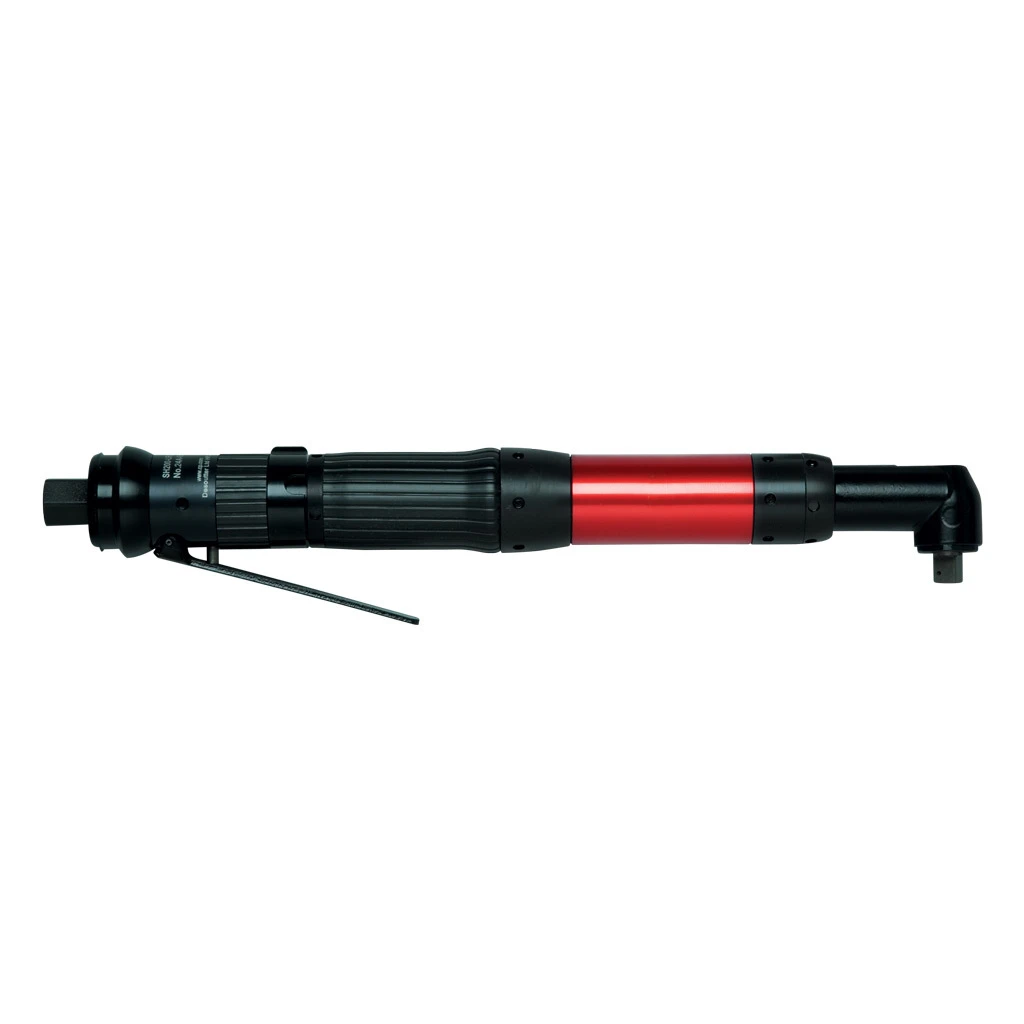
\includegraphics[width=\linewidth,height=2.6cm,keepaspectratio]{figures/additional/stationaryNutRunner.png}\\[2pt]\small (a)}\hfill%
    % TODO(figure): panel (b), a multi-spindle tightening station.
    \fbox{\parbox[c][3cm][c]{0.21\textwidth}{\centering\small (b) Placeholder:\\ multi-spindle station}}\hfill%
    % TODO(figure): panel (c), an industrial robot with a screwdriving end effector.
    \fbox{\parbox[c][3cm][c]{0.21\textwidth}{\centering\small (c) Placeholder:\\ robot with screwdriving end effector}}\hfill%
    % TODO(figure): panel (d), a fixture that presents the part in a fixed pose.
    \fbox{\parbox[c][3cm][c]{0.21\textwidth}{\centering\small (d) Placeholder:\\ fixture presenting the part}}%
    \caption{How threading is automated today: (a) a stationary nutrunner (image from~\cite{IntlAirTool}), (b) a multi-spindle station that tightens several fasteners of one part at once, (c) a robot with a screwdriving end effector, and (d) a fixture that presents the part in a fixed pose. Each solution is built for one fastener type and a known part pose.}%
    \label{fig:threading-automation}%
\end{figure}%

People handle the cases that dedicated equipment cannot. They pick up a nut, place it on a bolt, and turn it with their fingers, and they use the same hands to operate a wrench or a screwdriver. A robot with a dexterous, multi-fingered hand could in principle do the same. It could work with the parts and tools that were designed for people, in workcells that were designed for people, without a dedicated tool for every fastener~\cite{BicchiKumar2000,Weinberg2024}. Learning-based control has made in-hand manipulation with such hands practical in simulation and on hardware~\cite{Chen2021,Handa2024,Weinberg2024}. Robots have fastened screws with manual screwdrivers~\cite{Tang2023,Tang2024screwdriving}, and a single learned policy has manipulated a range of everyday tools with a dexterous hand~\cite{Kedia2026}. The vision behind this thesis is a dexterous robot that helps in manufacturing and assembly in a world built for humans. Threading a nut by hand is one of the basic skills such a robot needs. For humans the skill is trivial, but it is not for robots. This is an instance of Moravec's paradox: it is comparatively easy to make computers perform well on tasks that people find intellectually demanding, and difficult to give them the perception and mobility skills of a small child~\cite{Moravec1988}. Industrial fastening shows both sides of this paradox. A nutrunner on a fixture drives a fastener without difficulty, because the cell design has already solved the hard part: the part is held in a known pose and the fastener is presented in a known orientation. Without this structure, a robot has to find the hole, align the fastener, and engage the thread, which a person does without thinking. If a dexterous robot is to thread, it has to learn the skill, and the next section explains why that is hard.

\section{Problem: How Can a Robot Learn Threading?}\label{sec:problem-setup}

Teaching a robot to thread a nut with a dexterous hand raises three difficulties at once. First, the skill has to be learned in simulation and transferred to hardware, although thread contact is very hard to simulate. Second, the dexterous hand has a high-dimensional action space and countless ways to solve the task. Third, threading is a long-horizon cyclic task. The following subsections treat the three difficulties in turn, and each ends with the requirement it puts on the method.

\subsection{Simulation}\label{sec:difficulty-sim2real}

Learning a contact-rich skill directly on hardware is slow and unsafe. \Ac{RL} needs many trials, every trial costs robot time and wear, and exploration produces collisions and excessive forces~\cite{Kober2013}. Simulation removes these limits. GPU-parallel simulators run thousands of environments at once and have made \ac{RL} feasible for dexterous manipulation and for contact-rich assembly~\cite{Handa2024,Petrenko2023,Narang2022}.

Thread contact, however, is among the hardest interactions to simulate. Engaged threads produce thousands of simultaneous contacts, and simulating them faithfully needs dedicated contact methods, such as the signed-distance-field contacts with which Factory simulates 1000 nut-and-bolt assemblies in real time on one GPU~\cite{Narang2022}.

The GPU-parallel engines that make this scale possible, such as PhysX and MuJoCo, model contact through interpenetration. When two bodies overlap, the solver measures the penetration depth and generates a repulsive force that pushes the bodies apart again (Figure~\ref{fig:depenetration}).
% TODO(cite): penetration-based contact resolution in PhysX and MuJoCo (soft or penalty-like contact, depenetration velocity, contact offsets).
Contact is therefore never strictly rigid. It tolerates a small overlap, and the repulsive force grows with that overlap.

\begin{figure}[htb]%
    \centering%
    % TODO(figure): illustrate depenetration in a physics engine. Two bodies overlap by a penetration depth d, the solver generates a repulsive force or velocity along the contact normal that grows with d, and the bodies are pushed apart again.
    \fbox{\parbox[c][4cm][c]{0.7\textwidth}{\centering\small Placeholder:\ depenetration in a physics engine\ (penetration depth, contact normal, repulsive force)}}%
    \caption{How a physics engine resolves contact. Two bodies that overlap by a penetration depth $d$ receive a repulsive force along the contact normal that grows with $d$ and pushes them apart.}%
    \label{fig:depenetration}%
\end{figure}%

For large bodies this tolerance is harmless. For threads it is not, because the thread geometry is small. The pitch is 3 to 4\,mm for the nuts used in this thesis, and the flanks and crests are smaller still. At this scale, the overlap that the solver tolerates is no longer negligible against the geometry. A nut that is pushed along the axis can sink into the opposing flank and slide across the crest into the next groove, instead of following the helix. The repulsive force does not forbid this path, it only makes it more expensive. In simulation, the nut can thus phase through the threads.

A learning policy finds such shortcuts. If the reward pays for axial progress of the nut, the policy can collect it by pushing the nut through the threads rather than by turning it along the helix (Figure~\ref{fig:thread-exploit}). The resulting behavior solves the simulated task and fails on hardware, where the threads are rigid and the nut advances only by rotating. Faithful thread contact therefore needs dedicated contact methods and is easy to exploit, and any simplification of the thread opens a gap in contact between simulation and reality. A deployed policy also has to perceive the nut through a camera, and rendered images differ from real ones, which opens a second gap in perception. Collecting real data to close these gaps would bring back the cost that simulation was meant to avoid.

\begin{figure}[htb]%
    \centering%
    % TODO(figure): short illustration of thread geometry. Show the nut and bolt thread profiles with pitch and flank, a reward that pays for axial progress, and the exploit path in which the nut interpenetrates the flank and crosses into the next groove instead of following the helix.
    \fbox{\parbox[c][4cm][c]{0.7\textwidth}{\centering\small Placeholder:\ thread geometry and the interpenetration exploit\ (pitch, flank, helical path versus path through the thread)}}%
    \caption{How interpenetration can be exploited in thread simulation. A reward for axial progress of the nut is collected on the helical path by turning the nut, but also on a shortcut in which the nut interpenetrates the thread flank and crosses the crest into the next groove.}%
    \label{fig:thread-exploit}%
\end{figure}%

\emph{Requirement:} a thread model that is cheap enough for massively parallel \ac{RL} and cannot be exploited through interpenetration, and a transfer recipe that carries the learned skill to hardware without real-world data.

\subsection{Threading with a Dexterous Hand}\label{sec:difficulty-dexterity}

A multi-fingered hand on an arm has far more actuated joints than a parallel-jaw gripper, and its action space is correspondingly high-dimensional~\cite{Chen2021,Chen2023}. The task also has a large solution space. People thread a nut with a single finger, with a pinch between thumb and index finger, or with a grasp of several fingers, depending on how strongly the thread resists.
% TODO(cite): human grasp strategies for threading a nut (single finger, pinch, multi-finger grasp) as a function of thread resistance. Feix2016 is a general grasp taxonomy and does not cover threading.
A policy that may choose among all of these strategies has to explore a vast space of finger motions, and a reward that steers it toward one reliable strategy is hard to design~\cite{Kober2013}.

A dexterous hand also has to acquire the grasp, keep it under load while the nut turns, and release it again. Learned assembly with parallel-jaw grippers does not face this part of the problem. There, the threading or insertion policy starts every episode with the part already held, so it learns to move a part that is grasped, and grasping, holding, and re-grasping are not part of what it learns~\cite{Narang2022,Noseworthy2025,Tang2023industreal}. Learned dexterous threading has so far addressed the spinning of an already engaged fastener~\cite{Hsieh2026} and goal-conditioned screwing of furniture parts~\cite{Lum2026}.

\emph{Requirement:} a learned policy that controls the hand and the arm together, with the solution space narrowed to one grasp strategy, the pinch grasp, which the policy has to acquire, hold, and release.

\subsection{Threading as a Long-Horizon Cyclic Task}\label{sec:difficulty-horizon}

A long-horizon cyclic task repeats a fixed sequence of phases many times while the task state advances from one repetition to the next. Threading with a pinch grasp is such a task. One turn is limited by the range of the wrist and the fingers, so the hand has to approach the nut, grasp it, turn it, release it, and return for the next grasp, cycle after cycle. Meanwhile the nut advances along the thread by a fraction of a pitch in every cycle, so no two cycles start from the same state. Many tasks in assembly and everyday manipulation share this structure, for example driving a screw, turning a crank, winding a cable, or wiping a surface.
% TODO(cite): repetitive cyclic manipulation tasks in assembly and everyday settings.

Three properties make such tasks hard. First, errors compound across cycles. A grasp that lands slightly off the intended faces, a release that disturbs the nut, or a return that brings the fingers back at the wrong height carries over into the next cycle and accumulates. For a learned policy this is worse, because small deviations lead it to states it was not trained on, where its errors grow further~\cite{Ross2011}. Second, failures concentrate at the transitions between phases, where the contact between hand and nut is made or broken, rather than within a single phase. Third, a single \ac{RL} policy for the whole task needs a reward that covers every phase and every transition, and it has to assign the outcome of a late cycle to decisions made many steps earlier. Reward shaping over many phases and credit assignment over the full horizon break down for such a policy~\cite{Kober2013}.
% TODO(cite): reward shaping and credit assignment for a single RL policy over long multi-phase horizons.

The common answer is to decompose the task into skills, train one policy per skill, and chain the policies at deployment~\cite{Chen2023}. Chaining moves the difficulty to the transitions. The final state of one policy has to lie in the region where the next policy succeeds, which needs extra machinery that fine-tunes the sub-policies for their neighbors~\cite{Chen2023}, and several policies together with a switching logic have to be deployed. A second answer is to imitate complete long-horizon demonstrations with one generative policy~\cite{Chi2024,Black2026}. This avoids the reward problem, but it needs demonstrations of the whole task, and teleoperated demonstrations of forceful dexterous manipulation are hard to collect~\cite{Kedia2026}.

\emph{Requirement:} a training signal that is easy to specify phase by phase, and one deployable policy that sustains many cycles without switching between separate policies.

Taken together, the three requirements point to one approach: decompose the task where the training signal is generated, and unify it where the policy is deployed.

\section{Approach}\label{sec:approach}

This thesis decomposes the task during data generation and unifies it at deployment, as Figure~\ref{fig:overview} summarizes. Each part of the approach answers one of the difficulties of Section~\ref{sec:problem-setup}. A simplified kinematic thread model couples the axial travel of the nut to its rotation while keeping the finger--nut contacts, which makes massively parallel training with \ac{PPO} feasible (Section~\ref{sec:difficulty-sim2real}). A privileged \ac{RL} teacher, which observes the nut pose from the simulator, learns the pinch-grasp turn: approach, grasp, rotation, and goal reaching (Section~\ref{sec:difficulty-dexterity}). Scripted controllers release the nut and return the hand. Chained with the teacher, they form a hybrid teacher that generates complete multi-cycle demonstrations whose phase boundaries are triggered by physical events.
A single visuomotor student is then distilled from these demonstrations by \ac{CFM}~\cite{Lipman2023}. This teacher--student structure follows earlier work that distills privileged policies into sensor-based students~\cite{Singh2025,Lum2024}. The student cannot observe the true nut pose, so it replaces the teacher's privileged nut state with perception. It acts from proprioception and a fixed \acs{RGBD} camera whose model is calibrated against the physical cell. The depth image is converted into a metric point cloud~\cite{Ze2024}, and the rendering is randomized during data generation~\cite{Singh2025}, so that the student sees similar inputs in simulation and on hardware. Teacher, student, and robot share one Cartesian action path. The student is therefore meant to run the whole cycle on hardware without privileged state, without switching between policies, and without real-world data.

\begin{figure}[htb]%
    \centering%
    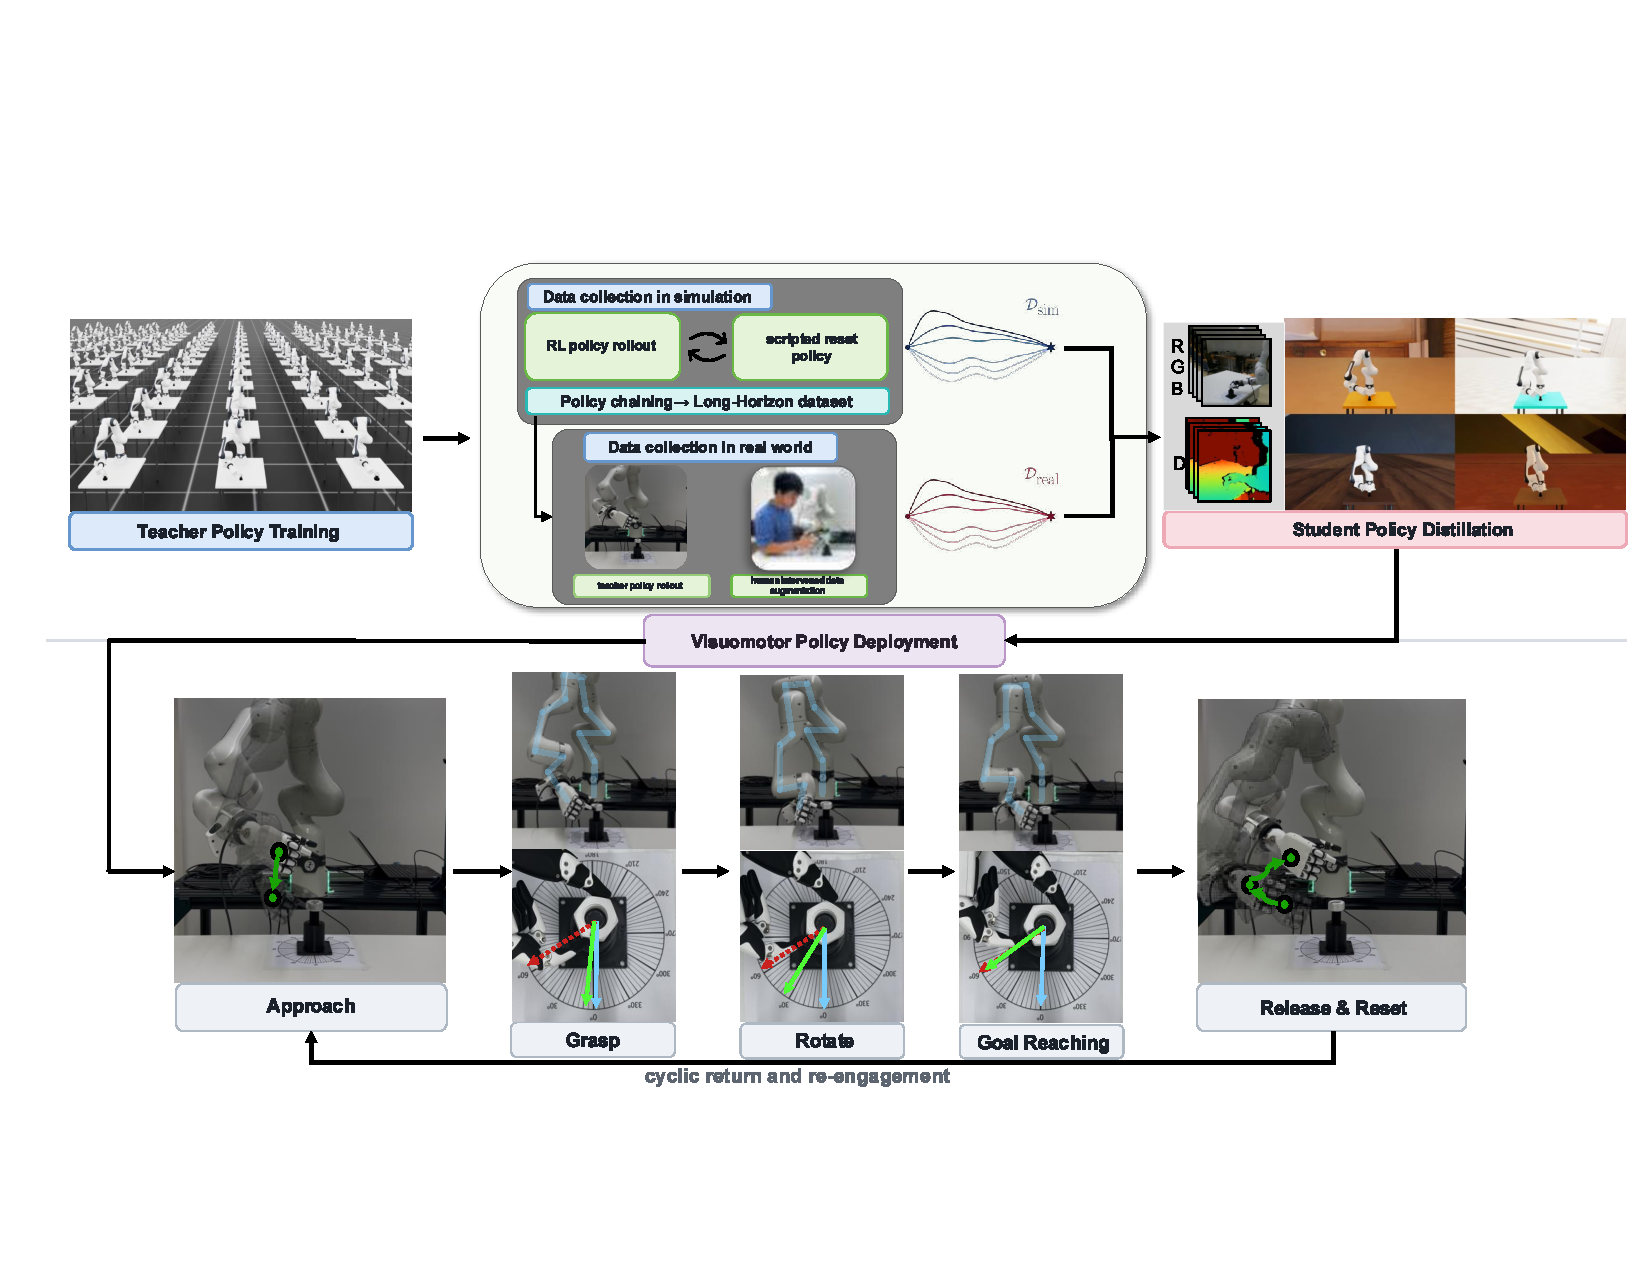
\includegraphics[width=\textwidth,trim=17bp 85bp 5bp 117bp,clip]{figures/SimThreadTeaser.pdf}%
    \caption{Overview of the approach: decompose during data generation, unify at deployment. Top: a privileged \acs{RL} teacher is trained in parallel simulated workcells. During data collection its rollouts are chained with scripted release-and-reset controllers into long-horizon demonstrations $\Dsim$. A conditional flow-matching student is distilled from them and acts from RGB and depth. Bottom: the phases of one cycle on the physical robot, approach, grasp, rotation, goal reaching, and release-and-reset, after which the hand returns for the next cycle.}%
    \label{fig:overview}%
\end{figure}%
% TODO(figure): the teaser graphic is the project's publication figure; check that it does not show a real-world replay or correction branch, and edit it if it does. Also check that it does not print robot, hand, or camera product names, which first appear in Chapter 5.

\section{Research Questions}\label{sec:research-questions}
% TODO(note): temporary review note, remove before submission.
\noindent\colorbox{yellow}{\parbox{\dimexpr\linewidth-2\fboxsep}{\textbf{Note:} Perhaps this section should be removed from the introduction.}}

The approach rests on two claims, that one student can replace a chain of policies and that it can be trained on simulated data alone, and on one design choice, the student that performs the unification. Three research questions test them.

\begin{description}
  \item[RQ1 (long horizon).] Does one student distilled from complete multi-cycle demonstrations sustain consecutive threading cycles better than a single-cycle policy that is invoked repeatedly?
  \item[RQ2 (student design).] Which student design distills the hybrid-teacher demonstrations into a policy that sustains the cyclic task? The ablations designed for it replace the flow-matching action head with deterministic regression on \ac{LSTM} and Transformer backbones, and the point-cloud encoder with an image-space encoder.
  \item[RQ3 (sim-to-real).] Can a student trained on simulated demonstrations only transfer zero-shot to the physical hand--arm system?
\end{description}

RQ1 tests the answer to the long-horizon difficulty, RQ2 asks which student makes the unification work, and RQ3 tests the answer to the transfer difficulty. The experiments for RQ1 and RQ2 run in simulation (Chapter~\ref{ch:sim}), and those for RQ3 on hardware (Chapter~\ref{ch:real}). The answer to the dexterity difficulty, the privileged teacher, is tested by the teacher training that Chapter~\ref{ch:sim} reports before the student experiments.

\section{Contributions}\label{sec:contributions}

The thesis makes the following contributions.

\begin{enumerate}
  \item A formulation of cyclic nut threading as an ordered sequence of phases with explicit cyclic and episodic tracking errors, and a hybrid teacher that combines a privileged \ac{RL} policy for approach, grasp, rotation, and goal reaching with scripted controllers for release and return. The hybrid teacher generates coherent multi-cycle demonstrations with physically gated phase boundaries.
  \item A unified visuomotor student distilled by conditional flow matching from a point-cloud representation of an aligned \acs{RGBD} view, proprioception, a global trajectory-progress scalar, and a process-phase encoding. Controlled single-seed design studies compare offline flow students with online \ac{DAgger} variants, privileged observations, and a joint-space action contract. The comparison with deterministic regression heads and alternative vision encoders is \tbd.
  \item A zero-shot sim-to-real recipe for the student: a camera model calibrated against the physical cell, a metric point cloud cropped to the workspace, visual randomization of the rendered demonstrations, and a Cartesian action path shared by teacher, student, and robot.
  \item An evaluation of the student in simulation on the hexagonal training nut and on hardware across three nut sizes and four nut profiles, of which only the M24 hexagonal nut appears in the training data. The simulation results are reported in Chapter~\ref{ch:sim}. The hardware results are \tbd.
\end{enumerate}

This work was carried out together with the advisor, who developed substantial parts of the hybrid teacher, the distillation stack, and the hardware experiments. The acknowledgments state this attribution.

\section{Outline}\label{sec:outline}

This thesis comprises seven chapters: Introduction, State of the Art, Methodology, Experiments in Simulation, Experiments on Real Hardware, Discussion, and Conclusion and Future Work. This chapter motivated threading as a skill for dexterous robots, named the difficulties of learning it, and stated the approach and the research questions. Chapter~\ref{ch:sota} reviews the background and related work, Chapter~\ref{ch:method} presents the method, Chapters~\ref{ch:sim} and~\ref{ch:real} report the experiments in simulation and on hardware, Chapter~\ref{ch:discussion} interprets the results, and Chapter~\ref{ch:conclusion} concludes the thesis. The remainder of this section outlines these chapters in more detail.

Chapter~\ref{ch:sota} provides the background that the method builds on: the thread geometry that the thread model uses, \ac{RL} with privileged information, imitation learning and compounding error, generative action heads, and operational-space control. It then reviews related work on robotic assembly and threading, dexterous manipulation, visual representations for manipulation, long-horizon tasks and policy chaining, and teacher--student distillation.

Chapter~\ref{ch:method} presents the method, with each part answering one difficulty of Section~\ref{sec:problem-setup}: the problem formulation, the simulated system with its thread model and controller, the privileged teacher, the hybrid teacher and the generation of demonstrations, the distillation of the student by conditional flow matching, and the evaluation protocol.

Chapter~\ref{ch:sim} reports the experiments in simulation. It covers teacher training, the main ablations for RQ1 and RQ2, the design ablations of the student, and the comparison of offline and online distillation.

Chapter~\ref{ch:real} describes the hardware setup, the zero-shot transfer protocol, and the real-world evaluation for RQ3 on the training nut, across nut sizes and geometries, and under long-horizon stress.

Chapter~\ref{ch:discussion} interprets the results with respect to the research questions, discusses what they mean for robotic assembly, and states the limitations of the work.

Chapter~\ref{ch:conclusion} returns to the assembly motivation of this chapter, summarizes what a dexterous robot can now do in threading and what is still missing, and outlines future work.
%
% !TeX spellcheck = en_US
\chapter{State of the Art}\label{ch:sota}%

This chapter provides the background that the method of Chapter~\ref{ch:method} builds on and places the thesis within related work. Section~\ref{sec:theory} introduces the theoretical concepts in the order in which the method uses them: the geometry of threaded joints that the thread model reproduces, reinforcement learning for the teacher, imitation learning for the distillation, action chunking and generative action heads for the student, and operational-space control for the action path that teacher, student, and robot share. Section~\ref{sec:related} reviews related work along the three difficulties that threading poses for a robot: it covers robotic assembly and threading, dexterous manipulation with learned policies, visual representations for manipulation, long-horizon tasks and policy chaining, and teacher--student distillation, and it closes with the gap that this thesis addresses.

\section{Theoretical Background}\label{sec:theory}

\subsection{Threaded Joints and Thread Geometry}\label{sec:thread-background}

Screws are divided into fastening screws and motion screws, and a nut on a bolt is a fastening joint~\cite{Niemann2019}. Threaded fasteners make a joint nonpermanent, so that it can be released again for field assembly, disassembly, maintenance, and adjustment~\cite{Budynas2020}. Their threads are standardized, for example in the ISO metric M series~\cite{Budynas2020}, whose geometry Figure~\ref{fig:iso-thread} shows. The thread converts a large circumferential motion into a small axial motion, and a small circumferential force into a large axial force~\cite{Niemann2019}. Assembling a threaded joint and securing it are treated as separate design topics~\cite{Niemann2019}. This thesis addresses the assembly motion, turning the nut along the thread, and not the securing of the joint.

\begin{figure}[htb]%
    \centering%
    % TODO(figure): replace the \fbox placeholder by a drawing of threads and their geometry according to the ISO standards (e.g. the ISO metric basic profile with pitch, flank angle, major, pitch, and minor diameter). Images need a license or a citable source, which then goes into the caption.
    \fbox{\parbox[c][5cm][c]{0.7\textwidth}{\centering\small Placeholder:\\ threads and thread geometry according to the ISO standards}}%
    \caption{Threads and thread geometry according to the ISO standards. Placeholder.}%
    \label{fig:iso-thread}%
\end{figure}%

The quantity that links rotation and axial travel is the pitch $\rho$, the distance between adjacent threads~\cite{Budynas2020}. For a single-start thread, adjacent threads are successive turns of one helix. A nut that turns by an angle $\Delta\theta$ about the bolt axis therefore advances along the axis by $\rho\,\Delta\theta/(2\pi)$, that is, by one pitch per revolution.
% TODO(cite): lead equals pitch for a single-start thread (Shigley Ch. 8 thread definitions); verify the passage before citing Budynas2020 for it.
Because a partial turn advances the nut by only a fraction of a pitch, the axial position at which a hand must grasp the nut changes with every turn.

\subsection{Reinforcement Learning}\label{sec:rl-background}

In \ac{RL}, an agent learns a behavior from interaction and a scalar reward, not from demonstrations~\cite{Sutton2018,Kober2013}. At every step an agent observes its environment, chooses an action, and receives a reward that rates the outcome. The agent has to discover the actions that lead to high reward by trying them, and it has to attribute a reward to the earlier actions that made it possible.

The interaction is formalized as a \ac{MDP} $(\mathcal{X}, \mathcal{A}, P, r, \gamma)$ with state space $\mathcal{X}$, action space $\mathcal{A}$, transition kernel $P(\vec{x}_{t+1}\mid \vec{x}_t,\vec{a}_t)$, reward $r(\vec{x}_t,\vec{a}_t)$, and discount factor $\gamma\in[0,1)$~\cite{Sutton2018}. The Markov property states that the next state depends only on the current state and action, not on the earlier history. A stochastic policy $\pi(\vec{a}\mid\vec{x})$ maps states to distributions over actions. Executing it generates a trajectory $\tau=(\vec{x}_0,\vec{a}_0,r_0,\vec{x}_1,\dots)$, and the goal is a policy that maximizes the expected discounted return
\begin{equation}\label{eq:rl-objective}
  J(\pi)=\E_{\tau\sim p_\pi}\!\left[\sum_{t=0}^{\infty}\gamma^{t}r_t\right].
\end{equation}
The discount factor sets how far ahead the agent plans. A reward that lies $t$ steps in the future is weighted by $\gamma^{t}$, so rewards beyond roughly $1/(1-\gamma)$ steps contribute little.

Value functions measure how good a state or an action is under a given policy. The state value $V^{\pi}(\vec{x})=\E_\pi[\sum_{l\geq0}\gamma^{l}r_{t+l}\mid\vec{x}_t=\vec{x}]$ is the expected return when the policy starts in $\vec{x}$. The action value $Q^{\pi}(\vec{x},\vec{a})$ is the expected return when the agent first takes $\vec{a}$ and then follows $\pi$. Their difference is the advantage
\begin{equation}\label{eq:advantage}
  A^{\pi}(\vec{x},\vec{a})=Q^{\pi}(\vec{x},\vec{a})-V^{\pi}(\vec{x}),
\end{equation}
which is positive for actions that are better than the policy's average behavior in that state and negative for worse ones. The state value satisfies the Bellman equation $V^{\pi}(\vec{x}_t)=\E_\pi[r_t+\gamma V^{\pi}(\vec{x}_{t+1})]$, which relates the value of a state to the reward of one step and the value of its successor~\cite{Sutton2018}. This recursion lets a value function be learned from single transitions instead of complete trajectories.

Value functions rate states and actions, but the policy itself can be improved directly by gradient ascent on the expected discounted return $J$ of \eqref{eq:rl-objective}. This requires a differentiable policy $\pi_\theta$, here a neural network with parameters $\theta$, and a gradient of $J$ that can be estimated from sampled trajectories. The likelihood-ratio form of the policy gradient,
\begin{equation}\label{eq:policy-gradient}
  \nabla_\theta J(\pi_\theta)=\E_{\tau\sim p_{\pi_\theta}}\!\left[\sum_{t}\nabla_\theta\log\pi_\theta(\vec{a}_t\mid\vec{x}_t)\,\Psi_t\right],
\end{equation}
estimates this gradient from sampled trajectories alone, without a model of the transition kernel~\cite{Williams1992,Sutton2018}. The weight $\Psi_t$ scores the action $\vec{a}_t$. With the return that follows step $t$ as $\Psi_t$, as in REINFORCE~\cite{Williams1992}, the estimate is unbiased but has high variance, because the return accumulates the randomness of every later action and transition.

Actor--critic methods reduce this variance by learning a value function alongside the policy. The actor is the policy $\pi_\theta$, and the critic is a value network $V_\phi$ that is regressed onto the observed returns. The critic replaces the return in $\Psi_t$ by an estimate of the advantage \eqref{eq:advantage}, that is, of how much better an action turned out than the critic expected. After one step, the critic compares its expectation $V_\phi(\vec{x}_t)$ with the observed reward plus its estimate of the next state. The difference is the temporal-difference residual $\delta_t=r_t+\gamma V_\phi(\vec{x}_{t+1})-V_\phi(\vec{x}_t)$, which is positive when the step went better than expected. \Ac{GAE}~\cite{Schulman2016} averages these residuals over the following steps with exponentially decaying weights,
\begin{equation}\label{eq:gae}
  \hat{A}_t=\sum_{l=0}^{\infty}(\gamma\lambda_{\mathrm{GAE}})^{l}\,\delta_{t+l},
\end{equation}
where $\lambda_{\mathrm{GAE}}\in[0,1]$ trades the bias of the critic against the variance of the observed returns.

The critic is needed only to compute $\hat{A}_t$ during training and is discarded afterwards. It may therefore receive information that the actor will not have at deployment. In an asymmetric actor--critic~\cite{Pinto2017}, the critic observes the full, noise-free simulator state, while the actor acts only on the observations available to it. The privileged critic gives more accurate value estimates and therefore better advantages for the actor, but the actor never depends on the privileged state.

\Acf{PPO}~\cite{Schulman2017} is an on-policy actor--critic algorithm. On-policy methods estimate the gradient from data collected by the current policy, so every batch becomes outdated as soon as the policy changes. \Ac{PPO} reuses each batch for several epochs of minibatch updates and keeps the updated policy close to the one that collected the data. It maximizes the clipped surrogate objective
\begin{equation}\label{eq:ppo}
  L^{\mathrm{clip}}(\theta) = \E_t\!\left[\min\!\left(\eta_t(\theta)\hat{A}_t,\; \operatorname{clip}\!\left(\eta_t(\theta),1-\epsilon,1+\epsilon\right)\hat{A}_t\right)\right],
  \qquad \eta_t(\theta)=\frac{\pi_\theta(\vec{a}_t\mid\vec{x}_t)}{\pi_{\theta_{\mathrm{old}}}(\vec{a}_t\mid\vec{x}_t)},
\end{equation}
where $\eta_t(\theta)$ is the probability ratio between the new and the old policy and $\epsilon$ is the clipping parameter. Once the ratio leaves the interval $[1-\epsilon,1+\epsilon]$ in the direction that the advantage favors, the objective stops growing, and the gradient no longer pushes the policy further. The full loss adds a squared-error loss for the critic and an optional entropy bonus that keeps the policy stochastic,
\begin{equation}\label{eq:ppo-loss}
  L(\theta,\phi)=-L^{\mathrm{clip}}(\theta)+c_V\,\E_t\!\left[\big(V_\phi(\vec{x}_t)-\hat{R}_t\big)^{2}\right]-c_H\,\E_t\!\left[\mathcal{H}\big(\pi_\theta(\cdot\mid\vec{x}_t)\big)\right],
\end{equation}
with the return target $\hat{R}_t=\hat{A}_t+V_{\phi}(\vec{x}_t)$, the critic coefficient $c_V$, the entropy coefficient $c_H$, and the policy entropy $\mathcal{H}$~\cite{Schulman2017}. One training epoch collects a rollout of fixed length from every environment, computes the advantages \eqref{eq:gae}, and then runs several passes of minibatch gradient descent on \eqref{eq:ppo-loss}. On-policy learning needs many samples, and GPU-parallel simulators supply them by stepping thousands of environments at once. On such simulators, \ac{RL} has trained in-hand reorientation that transferred to hardware~\cite{Handa2024} and regrasping and throwing with simulated hand--arm systems~\cite{Petrenko2023}.

The reward is the only specification of the task that the agent receives, and its design largely decides whether learning succeeds~\cite{Kober2013}. A sparse reward that pays only on success is easy to specify, but in a high-dimensional action space random exploration almost never reaches success, so the agent receives no learning signal. Reward shaping adds dense terms that pay for intermediate progress, such as moving the hand toward the object or turning it toward the goal. Shaping can, however, change which policy is optimal. Ng et al.~\cite{Ng1999} show that a shaping term of the form $F(\vec{x}_t,\vec{x}_{t+1})=\gamma\Phi(\vec{x}_{t+1})-\Phi(\vec{x}_t)$, with an arbitrary potential function $\Phi$ over states, leaves the optimal policy unchanged, and that other shaping terms carry no such guarantee. A term that is not of this form may be exploited. The agent optimizes the reward as written rather than the task as intended. A term that pays for every reduction of a distance, for example, pays again each time the agent moves away and comes back, so a policy can collect it by oscillating. In simulation the agent can also exploit inaccuracies of the physics, as the interpenetration through the thread flanks of Section~\ref{sec:difficulty-sim2real} illustrates.

\ac{RL} thus produces a policy from a reward alone, at the cost of many simulated trials and a carefully shaped reward. When an expert policy or recorded demonstrations are available, a policy can instead be learned by supervised imitation, which the next subsection introduces.

\subsection{Imitation Learning}\label{sec:il-background}

\Ac{IL} is the problem of learning a policy from the demonstrations of an expert rather than from a reward. \Ac{IL} methods differ in how they use the demonstrations. The simplest method, \ac{BC}, reduces \ac{IL} to supervised learning~\cite{Ross2011}. It treats every demonstrated pair of observation and expert action as a labeled training example and fits the learned policy, called the student, to these labels. Given a dataset $\Dset=\{(\obs_t,\act^{*}_t)\}$, \ac{BC} solves the regression problem
\begin{equation}\label{eq:bc}
  \theta^{*}=\argmin_\theta \E_{(\obs,\act^{*})\sim\Dset}\!\left[\ell\!\left(\piS(\obs),\act^{*}\right)\right],
\end{equation}
with a per-sample loss $\ell$ such as the squared error. \ac{BC} is trained on the states that the expert visits but evaluated on the states that the student visits. Small prediction errors move the student into states that are not covered by the demonstrations, and the errors compound. Ross et al.~\cite{Ross2011} show that the expected cost of a \ac{BC} policy with per-step error $\varepsilon$ can grow as $O(T^2\varepsilon)$ over a horizon $T$. For a cyclic task, small deviations in grasp height or nut angle carry over from one cycle into the next.

\Ac{DAgger}~\cite{Ross2011} counters this by querying the expert on the states that the student itself visits. The environment is driven by a mixture that executes the expert's action with probability $\beta$ and the student's action otherwise, the expert labels every visited state, and the student is retrained on the aggregated dataset. The expected cost then grows only linearly in the horizon. \ac{DAgger} requires an expert that can be queried at arbitrary states. A policy in simulation satisfies this requirement, a recorded demonstration does not.

\subsection{Action Chunking}\label{sec:chunking-background}

A policy that predicts one action per observation is queried at every control step. An action-chunking policy instead predicts a sequence of $H$ future actions, the action chunk $[\act_t,\dots,\act_{t+H-1}]$, from the observation $\obs_t$~\cite{Zhao2023}. It executes the first $H_{\mathrm{e}}\leq H$ actions of the chunk without querying the policy again and then predicts a new chunk from the current observation. The policy thus plans further ahead than it acts, which keeps consecutive actions consistent while the policy still responds to new observations at every query~\cite{Chi2024}. Chunking has three benefits for imitation learning and one cost.

First, chunking counters the compounding errors of \ac{BC} (Section~\ref{sec:il-background}). A policy that executes $H_{\mathrm{e}}$ actions per query makes only $T/H_{\mathrm{e}}$ decisions over a task of $T$ steps. The effective horizon of the task shrinks by the factor $H_{\mathrm{e}}$, and fewer errors can compound~\cite{Zhao2023}.

Second, chunking handles demonstrations that are not Markovian in the observation. Human demonstrators pause in the middle of a demonstration, for example during teleoperation, and the observation does not show how long the pause has lasted. A single-step policy learns that it stands still in such a state, but not for how long, and it can get stuck~\cite{Zhao2023,Chi2024}. A chunk covers the pause together with the motion that follows it, so the policy can learn to resume. Similarly, when the demonstrations contain several valid behaviors, a policy that samples every action independently can switch between them from one step to the next and produce jittery motion. A chunk is sampled as a whole and follows one behavior~\cite{Chi2024}.

Third, chunking decouples inference from the control rate. A large policy, such as a vision-language-action model, can need longer for one inference than one control period. A chunk supplies actions for several control periods, so the robot keeps moving while the next chunk is computed~\cite{Black2025}. In this way, a vision-language-action model controls robots at up to 50\,Hz~\cite{Black2026}.

The cost of chunking is reactivity. While the actions of a chunk execute, the policy does not observe their effect and cannot respond to a disturbance before its next query. In tasks with uncertain contact, a long execution horizon therefore trades robustness against compounding errors for responsiveness to the contact. Two remedies keep the chunk prediction and restore feedback. Temporal ensembling queries the policy at every step and executes an exponentially weighted average of all predictions for the current step from the chunks that are still valid~\cite{Zhao2023}. Real-time chunking generates the next chunk while the current one executes. It fixes the actions that will execute before the new chunk is ready and fills in the rest of the new chunk consistently with them, which avoids discontinuities at the switch between chunks~\cite{Black2025}. Predicting a chunk requires a model of the distribution over action sequences, which the generative action heads of the next subsection provide.

\subsection{Generative Action Heads: Diffusion and Flow Matching}\label{sec:generative-background}

A generative model learns a probability distribution from a set of samples and produces new samples from it. Diffusion models~\cite{Ho2020} do so by transforming Gaussian noise step by step into a data sample with a learned network. Conditioned on a text prompt, latent diffusion models generate high-resolution images that match the prompt~\cite{Rombach2022}.

In robot learning, the same principle generates actions instead of images. A generative action head learns the conditional distribution $p(\act\mid\obs)$ of the demonstrated actions given the observation and draws an action from it at run time. A regression head instead predicts a single action per observation, and the Gaussian policy of Section~\ref{sec:rl-background} represents only a single mode. The generative action head has two advantages. First, when the demonstrations contain several valid actions for the same observation, a sample takes one of them rather than their average~\cite{Chi2024}. The average of two valid actions need not be valid itself, for example: if an obstacle can be passed on either side, the average drives into it. Second, the head can generate a whole action chunk (Section~\ref{sec:chunking-background}) as one sample, so that all actions of the chunk follow the same mode~\cite{Chi2024}. Generative action heads are also used in large generalist policies, such as the vision-language-action model $\pi_0$, which is trained on data from many robots and tasks~\cite{Black2026}. Two families of generative action heads are common in robot learning, diffusion and flow matching. Both start from Gaussian noise and transform it step by step into an action, but they learn this transformation differently.

Diffusion Policy~\cite{Chi2024} learns to remove noise. During training, Gaussian noise is added to a demonstrated action, and a network that is conditioned on the observation predicts the added noise. The magnitude of the noise depends on a randomly drawn iteration index through the noise schedule, a hand-designed sequence of noise variances that fixes how much noise each iteration adds or removes. At run time, sampling starts from pure noise and applies the network over a fixed number of denoising iterations, each of which removes part of the predicted noise. The number of iterations sets the inference cost. Diffusion Policy predicts action chunks and executes several actions of a chunk before it predicts again.

Flow matching~\cite{Lipman2023,Lipman2024} learns the transformation from noise to action as a velocity field. Each noise sample can be pictured as a particle that moves during a flow time $\lambda$ from 0 to 1. A network $\vec{v}_\theta(\act,\lambda\mid\obs)$ predicts the velocity of the particle at position $\act$ and time $\lambda$, and integrating this velocity from a noise sample $\act^{0}$ at $\lambda=0$ yields an action $\act^{1}$ at $\lambda=1$. The velocity field that maps the noise distribution onto the demonstrated actions is unknown, but a training target can be built from pairs of a noise sample and a demonstrated action. The simplest construction connects the two by a straight line,
\begin{equation}\label{eq:fm-line}
  \act^{\lambda}=(1-\lambda)\act^{0}+\lambda\act^{1},\qquad \act^{0}\sim\mathcal{N}(\vec{0},\mat{I}),
\end{equation}
along which the velocity is the constant $\act^{1}-\act^{0}$. Training regresses the network onto this velocity at random points of random lines,
\begin{equation}\label{eq:fm-loss}
  L(\theta)=\E_{(\obs,\act^{1})\sim\Dset,\;\act^{0}\sim\mathcal{N}(\vec{0},\mat{I}),\;\lambda\sim U[0,1]}\left\|\vec{v}_\theta(\act^{\lambda},\lambda\mid\obs)-\left(\act^{1}-\act^{0}\right)\right\|_2^{2}.
\end{equation}
Many lines pass through the same point, so the network learns the average of their velocities. Lipman et al.~\cite{Lipman2023} show that this average is exactly the unknown velocity field, so the simple loss \eqref{eq:fm-loss} trains the correct model. At run time, an action is generated by drawing $\act^{0}\sim\mathcal{N}(\vec{0},\mat{I})$ and following the learned field with a few explicit Euler steps $\act^{\lambda+\Delta\lambda}=\act^{\lambda}+\Delta\lambda\,\vec{v}_\theta(\act^{\lambda},\lambda\mid\obs)$.

Diffusion and flow matching are closely related. A diffusion model corresponds to flow matching with a particular Gaussian path between noise and data, whose trajectories are curved~\cite{Lipman2023}. Figure~\ref{fig:diffusion-vs-fm} contrasts the two. The straight-line path of \eqref{eq:fm-line} gives flow matching three advantages. First, training is simpler. The regression target is the difference of two samples, and the path fixes how noise and data are mixed over the flow time, so no noise schedule has to be designed. Second, sampling is faster. A straight path can be followed with a few large integration steps, whereas a curved path needs many small ones. On image generation, flow matching reaches the sample quality of diffusion with fewer network evaluations~\cite{Lipman2023}. Third, sampling is the deterministic integration of an \ac{ODE} from a given noise sample. The number of integration steps can therefore be chosen at run time, which trades accuracy against inference time without retraining. Fast sampling matters for robot control, because a new action chunk must be ready within the control period. $\pi_0$ uses flow matching to generate action chunks for control at up to 50\,Hz~\cite{Black2026}.

In a policy, the flow-matching action head sits on top of a backbone. The backbone encodes the observation, for example camera images, the robot state, or a language instruction, into a condition vector $\cond$, which takes the place of $\obs$ in \eqref{eq:fm-loss}. The head is the velocity network $\vfield(\act^{\lambda},\lambda\mid\cond)$. It receives the noisy action or action chunk $\act^{\lambda}$, the flow time $\lambda$, and the condition, and it outputs a velocity of the same dimension as the action. The flow time is a scalar and is usually embedded with sinusoidal features before it enters the network~\cite{Black2026}. The velocity network is typically an \ac{MLP} or a Transformer. The condition enters it by concatenation with the input, by a feature-wise scaling and shifting of the hidden layers~\cite{Chi2024}, or as additional tokens that the action tokens attend to~\cite{Black2026}. The backbone is evaluated once per generated action chunk, the head once per integration step. Each additional step therefore costs only one evaluation of the head. $\pi_0$ follows this structure: a second set of Transformer weights, called the action expert, generates action chunks by flow matching and attends to the features of a pre-trained vision-language model~\cite{Black2026}. Section~\ref{sec:student} describes the backbone and the head of the student in this thesis.

\begin{figure}[htb]%
    \centering%
    % Generated by figures/diffusion_vs_flow_matching.py (exact models on a 2-D Gaussian-mixture toy problem).
    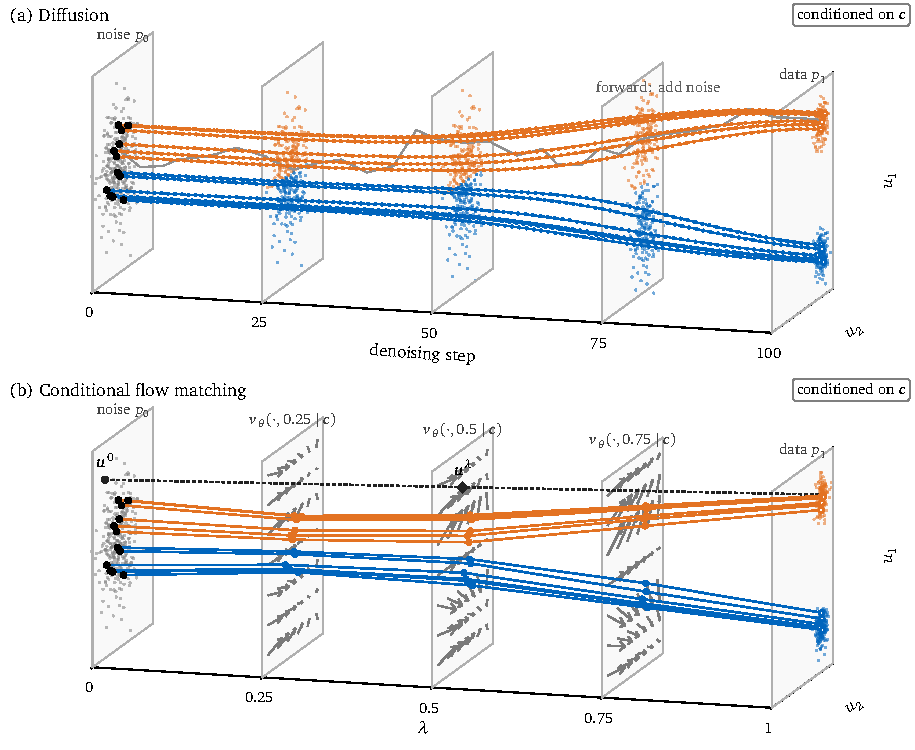
\includegraphics[width=\textwidth]{figures/diffusion_vs_flow_matching_3d.pdf}%
    \caption{Diffusion and conditional flow matching for a bimodal action distribution in a two-dimensional toy action space $(u_1,u_2)$. Generation time runs from left to right, from Gaussian noise $p_0$ to the demonstrated actions $p_1$, and each slice shows the action space at one point in time. (a) A diffusion model adds noise to demonstrated actions (gray path) and learns to reverse this process over many denoising steps along curved trajectories. The point clouds on the slices are intermediate denoising samples, colored by the mode they reach. (b) Conditional flow matching regresses a velocity field onto the straight path between a Gaussian sample and a data sample (dashed). Integrating the learned field (gray arrows on the slices at $\lambda=0.25$, $0.5$, and $0.75$) from noise reaches either mode in a few \acs{ODE} steps.}%
    \label{fig:diffusion-vs-fm}%
\end{figure}%

\subsection{Operational-Space Control}\label{sec:osc-background}

A policy controls a robot arm through its action space, and the choice of this space decides how much of the motion the policy has to learn itself. The most direct choice is the joint space. On a seven-DoF arm, the policy outputs seven joint position targets at every step, and a joint position controller tracks them in simulation and on the hardware. The policy then learns the complete motion of the arm, including the coordination of the joints that moves the end effector to where the task needs it. Joint-space actions impose no structure on this motion and leave the policy free to explore. Grasping pipelines that train arm and hand together with \ac{RL} use them. For example, a humanoid with two seven-DoF arms learns to grasp, lift, and hand over objects with joint position targets for its arm and hand joints~\cite{Lin2025}.

The alternative moves part of the motion into a controller that runs both during training and at deployment. The policy then commands a target in the operational space, the space in which the task is described~\cite{Khatib1987}. For assembly, this is the six-dimensional pose of the end effector, its position and orientation in Cartesian space, and the controller computes the joint torques that move the end effector toward the commanded pose. The action space shrinks from the number of joints to six dimensions, and it is expressed in the coordinates of the task, for example relative to a bolt. With an impedance controller in end-effector space, \ac{RL} learns contact-rich tasks with fewer samples than with joint-space actions~\cite{MartinMartin2019}.

Impedance is the second reason for this choice. A stiff position controller drives through an unexpected contact and can produce forces that damage the robot or the parts. An impedance controller instead makes the end effector behave as if it were attached to the target by a spring and a damper~\cite{Villani2016}. In steady contact, the force on the environment equals the stiffness times the deviation of the end effector from its target, so a small target offset produces only a small force. This protects the robot and the environment. It also gives the policy a way to apply force: a target that lies a small distance behind a contact surface presses the end effector against the surface with the stiffness times that distance. The policy thus regulates contact forces by placing targets, without commanding forces directly.

Task-space motion control with torque inputs and impedance control are treated in standard references~\cite{Lynch2017,Chung2016,Villani2016}. Impedance control is simplest in joint space. Assuming that gravity is compensated, the law
\begin{equation}\label{eq:joint-impedance}
  \vec{\tau}=\mat{K}_{q}\left(\vec{q}_{\mathrm{ref}}-\vec{q}\right)-\mat{D}_{q}\dot{\vec{q}}
\end{equation}
makes every joint behave like a spring with stiffness $\mat{K}_{q}$ and a damper with damping $\mat{D}_{q}$ around its reference $\vec{q}_{\mathrm{ref}}$, where $\vec{q}$ are the joint positions (Figure~\subref*{fig:impedance-model-joint}). The spring then acts on the joints, not on the end effector, and the stiffness felt at the end effector changes with the arm configuration. Operational-space impedance control instead defines the spring and the damper directly in the six-dimensional task space and maps them to the joints with the Jacobian. Joint space and operational space are related by the forward kinematics
\begin{equation}\label{eq:fk}
  \vec{x}=\vec{f}(\vec{q}),
\end{equation}
which gives the pose $\vec{x}$ of a frame on the robot for the joint positions $\vec{q}$. The Jacobian is the derivative of this map, $\mat{J}(\vec{q})=\partial\vec{f}/\partial\vec{q}\in\R^{6\times7}$. By the chain rule, it relates the velocities in the two spaces,
\begin{equation}\label{eq:jacobian}
  \dot{\vec{x}}=\frac{\partial\vec{f}}{\partial\vec{q}}\,\frac{\mathrm{d}\vec{q}}{\mathrm{d}t}=\mat{J}(\vec{q})\,\dot{\vec{q}}.
\end{equation}
The relation is linear in the joint velocities, but the Jacobian itself changes with the configuration. For the orientation, the time derivative of a parameterization such as Euler angles is not the angular velocity of the frame. Controllers therefore use the geometric Jacobian, which maps the joint velocities to the twist $\dot{\vec{x}}$ of the frame, its linear and angular velocity~\cite{Lynch2017}. By the principle of virtual work, its transpose maps a wrench $\vec{F}$ at the frame to the joint torques that produce it, $\vec{\tau}=\mat{J}^{\mathrm{T}}\vec{F}$~\cite{Lynch2017}. The frame can be any point on the robot, for example the point between the fingertips at which the hand holds the nut. A virtual spring and damper at this frame (Figure~\subref*{fig:impedance-model-task}), $\vec{F}=\mat{K}_p\vec{e}-\mat{K}_d\dot{\vec{x}}$ with the position and axis-angle orientation error $\vec{e}\in\R^6$ between target and current pose, therefore translates directly into joint torques, and the controller computes them at every step from the current Jacobian. On the seven-DoF arm, the six task dimensions leave one redundant degree of freedom, which a second term controls. The complete law, in the form that the thesis uses, is
\begin{equation}\label{eq:osc}
  \vec{\tau}=\mat{J}^{\mathrm{T}}\!\left(\mat{K}_p\vec{e}-\mat{K}_d\dot{\vec{x}}\right)+\mat{N}^{\mathrm{T}}\mat{M}\!\left(\mat{K}_{p,0}(\vec{q}_0-\vec{q})-\mat{K}_{d,0}\dot{\vec{q}}\right),
\end{equation}
where $\mat{K}_p$ and $\mat{K}_d=2\sqrt{\mat{K}_p}$ are diagonal stiffness and critical-damping gains, and the second term pulls the redundant degree of freedom toward a rest posture $\vec{q}_0$ through a nullspace projector $\mat{N}$ with posture gains $\mat{K}_{p,0}$ and $\mat{K}_{d,0}$. The joint-space inertia $\mat{M}$ converts the posture term from a joint acceleration into a torque.

\begin{figure}[htb]%
    \centering%
    % Source: figures/JointImpendanceControllerModel.svg and figures/ImpendanceControllerModel.svg, exported to PDF with Inkscape.
    \begin{subfigure}[b]{0.49\textwidth}
        \centering
        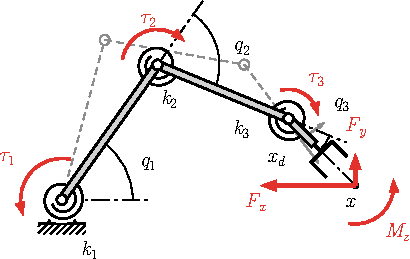
\includegraphics[width=\textwidth]{figures/JointImpendanceControllerModel.pdf}
        \caption{Joint-space impedance.}
        \label{fig:impedance-model-joint}
    \end{subfigure}\hfill
    \begin{subfigure}[b]{0.49\textwidth}
        \centering
        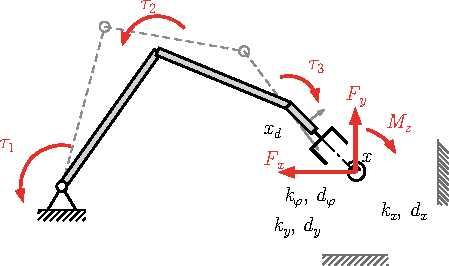
\includegraphics[width=\textwidth]{figures/ImpendanceControllerModel.pdf}
        \caption{Operational-space impedance.}
        \label{fig:impedance-model-task}
    \end{subfigure}
    \caption{Impedance control, illustrated on a planar arm with three joints. (a) A virtual spring and damper with stiffness $k_1,k_2,k_3$, the diagonal entries of $\mat{K}_q$, act directly on each joint, pulling it toward its reference $q_{\mathrm{ref}}$. (b) A virtual spring and damper with stiffness $k_x,k_y,k_\varphi$ and damping $d_x,d_y,d_\varphi$, the diagonal entries of $\mat{K}_p$ and $\mat{K}_d$, act on the controlled end-effector frame along each task direction instead. The resulting wrench $(F_x,F_y,M_z)$ is mapped to the joint torques $\tau_1,\tau_2,\tau_3$ through $\mat{J}^{\mathrm{T}}$.}%
    \label{fig:impedance-model}%
\end{figure}%

The nullspace projector decides how strongly the posture term interferes with the task. It is dynamically consistent when $\mat{N}^{\mathrm{T}}=\mat{I}-\mat{J}^{\mathrm{T}}\bar{\mat{J}}^{\mathrm{T}}$ with the inertia-weighted pseudoinverse $\bar{\mat{J}}=\mat{M}^{-1}\mat{J}^{\mathrm{T}}(\mat{J}\mat{M}^{-1}\mat{J}^{\mathrm{T}})^{-1}$ and joint-space inertia $\mat{M}$~\cite{Dietrich2015,RoboticSystemsLab2019}. Torques in the nullspace then produce no acceleration of the controlled frame. A projector built from a pseudoinverse of the Jacobian without inertia weighting needs no inertia model, but it decouples the nullspace from the task only statically, so that posture torques can still disturb the task during motion~\cite{Dietrich2015}. The controllers in simulation and on the physical robot both use the dynamically consistent projector (Section~\ref{sec:real-setup}). Equation~\eqref{eq:osc} is the Factory and FORGE controller~\cite{Narang2022,Noseworthy2025}. Scaling the spring and damper term by the task-space inertia $\mat{\Lambda}=(\mat{J}\mat{M}^{-1}\mat{J}^{\mathrm{T}})^{-1}$ and compensating the nonlinear dynamics yields the full operational-space formulation, in which the closed loop becomes a decoupled unit-mass system in every task direction~\cite{Lynch2017}.

\section{Related Work}\label{sec:related}

The related work is ordered along the difficulties of threading. Section~\ref{sec:related-assembly} reviews robotic assembly and threading, the application itself. Section~\ref{sec:related-dexterous} reviews learned dexterous manipulation (difficulty~(b)), Section~\ref{sec:related-vision} reviews visual representations for manipulation, and Sections~\ref{sec:related-chaining} and~\ref{sec:related-distillation} review long-horizon tasks and the teacher--student distillation with which this thesis addresses them (difficulty~(c)). Section~\ref{sec:related-gap} states the gap.

\subsection{Robotic Assembly and Threading}\label{sec:related-assembly}

Robotic assembly, for example peg-in-hole insertion, gear meshing, connector mating, and nut--bolt fastening, requires contact-rich interaction with high precision and accuracy~\cite{Tang2023industreal}. In mass production, dedicated fixtures position the parts precisely and thereby reduce the uncertainty of the hole pose~\cite{Manyar2023}. Learning-based methods train assembly policies in simulation. Factory~\cite{Narang2022} combines signed-distance-field collision detection, contact reduction, and a Gauss--Seidel solver to simulate 1000 nut-and-bolt assemblies in real time on a single GPU, and it learns nut-and-bolt assembly with \ac{RL} through separate pick, place, and screw subpolicies. FORGE~\cite{Noseworthy2025} trains force-guided exploration under pose uncertainty and demonstrates on a real robot a multistage planetary-gear assembly that includes nut threading, and IndustReal~\cite{Tang2023industreal} transfers simulation-trained assembly policies to a physical arm. All three use a parallel-jaw gripper.

Screwdriving with a manual screwdriver has been addressed with analytical models and force control, first with the tool rigidly attached to a robot arm~\cite{Tang2023} and then with the tool held by a Shadow Hand~\cite{Tang2024screwdriving}. For an industrial screwdriving tool on an impedance-controlled arm, a physics-informed learned model describes the motion of the screw tip~\cite{Manyar2023}. With multi-fingered hands, twisting the lids off bottle-like objects has been learned with two hands by sim-to-real \ac{RL}~\cite{Lin2024}, and unscrewing a bottle lid with one hand has been learned from teleoperated demonstrations with a visuomotor diffusion policy~\cite{Koczy2025}. Play2Perfect~\cite{Lum2026} pretrains a goal-conditioned dexterous manipulation policy through play and fine-tunes it for precise assembly, including screwing a furniture leg into a table fixture. It thus covers goal-directed screwing of a furniture leg, but not of small fasteners such as nuts. The only reviewed work that fastens nuts with a dexterous hand is DexScrew~\cite{Hsieh2026}. It mounts a 12-DoF hand on a robot arm and replaces the thread geometry by a revolute-joint proxy to learn a rotational finger gait with \ac{RL}. The gait assists teleoperation and supports the collection of real demonstrations for tactile behavior cloning. The \ac{RL} policy is rewarded for the angular velocity of the fastener rather than for reaching a target angle, its episodes end on failure or after a fixed time limit rather than on reaching a goal, and the nut is already installed on the bolt. Goal-directed threading over many grasp-and-release cycles, which this thesis addresses, is left open by these works.

\subsection{Dexterous Manipulation with Learned Policies}\label{sec:related-dexterous}

A multi-fingered hand is a general-purpose alternative to task-specific tooling, but it brings high-dimensional control and complex contact dynamics with it~\cite{BicchiKumar2000,Weinberg2024}. According to a recent survey, analytical models of motion and contact have failed to provide practical solutions for in-hand manipulation because they cannot cope with complex environments and uncertainty, and research has therefore shifted to learning~\cite{Weinberg2024}. Model-free \ac{RL} in simulation learns in-hand reorientation of more than two thousand objects~\cite{Chen2021}. DeXtreme~\cite{Handa2024} transfers agile in-hand reorientation from simulation to a comparatively affordable Allegro hand with a vision-based pose estimator, and DexPBT~\cite{Petrenko2023} learns regrasping and grasp-and-throw for simulated hand--arm systems with population-based training. DextrAH-G~\cite{Lum2024} and DextrAH-RGB~\cite{Singh2025} grasp a wide range of objects with a hand--arm system from depth and RGB images, respectively, and SimToolReal~\cite{Kedia2026} manipulates tool-like objects to random goal poses and generalizes zero-shot to real tools. Without learning, an arm-driven hand has executed a finger gait on a tool whose tip pivots on a supporting plane, using hybrid position/impedance control with reference finger forces~\cite{Xue2023}.

Several works name the high-dimensional action space of the hand or of the hand--arm system as a key challenge of dexterous manipulation~\cite{Chen2021,Lum2024,Chen2023}. Most of the works above learn one skill, such as grasping, reorienting an object, or moving a tool to goal poses. In-hand reorientation chains goals and counts consecutive successes~\cite{Handa2024}, but the object stays in the hand. Threading additionally requires the hand to release the part and acquire it again while the bolt constrains it, and the grasp must hold under the turning load in between. This thesis narrows the solution space to one grasp strategy, a thumb--index pinch, and lets the learned policy control this pinch together with the arm (Section~\ref{sec:system}).

\subsection{Visual Representations for Manipulation}\label{sec:related-vision}

A visuomotor policy must extract the task-relevant geometry from camera data, in threading the pose of the nut relative to the hand. Two families of encoders, and combinations of them, are used for this. Image-space encoders apply a convolutional backbone such as ResNet-18~\cite{He2016} to the RGB image, possibly with depth or other per-pixel channels added, and pool the feature map into a vector. They can start from ImageNet-pretrained weights, but from RGB alone they have to infer metric geometry from appearance, and when they are trained on rendered images they must be made robust to texture and lighting, for example by visual domain randomization~\cite{Tobin2017}. Point-cloud encoders back-project the depth image through the calibrated camera model into a set of 3D points, optionally attach the pixel color, and encode the set with a shared point network followed by global max pooling in the spirit of PointNet~\cite{Qi2017}. The \ac{DP3} encoder~\cite{Ze2024} is such a compact encoder, a three-layer \ac{MLP} with max pooling and a projection head, and it uses the point coordinates without color. In real-robot tests with one trial per condition, \ac{DP3} generalizes to unseen object colors and slightly changed camera views on which image- and depth-image-based Diffusion Policy~\cite{Chi2024} fail. The authors attribute the robustness to appearance to the omission of color and the spatial generalization to the 3D representation~\cite{Ze2024}. Adapt3R~\cite{Wilcox2025} combines the two families. Dense 2D features from a pretrained backbone are localized in 3D by the depth map and expressed in the end-effector frame before attention pooling. In simulation, this lets a policy transfer zero-shot to unseen robot arms and camera viewpoints, although its success rate on unseen arms is lower than on the training arm. The student of this thesis uses a point-cloud encoder in the style of \ac{DP3} whose points carry their pixel color, and Chapter~\ref{ch:sim} sets up its comparison with an image-space encoder and with an Adapt3R-style encoder.

\subsection{Long-Horizon Tasks and Policy Chaining}\label{sec:related-chaining}

A long-horizon task can be learned by one policy over the whole horizon or decomposed into skills, and each route has its own difficulties. One policy trained with \ac{RL} needs a reward that covers every phase, and it has to assign the outcome of a late phase to decisions made many steps earlier. AlphaNIST~\cite{Zhang2026} shows in simulation that a sparse binary task reward can suffice. It trains one policy from scratch on the 20 assembly tasks of the NIST Assembly Task Board~\#1, which require precise, contact-rich control of small, tight-fitting parts, and reaches 98.2\,\% overall training success without demonstrations, progress shaping, or scripted primitives. The same framework trains policies that complete ten assembly pairs in one episode without a prescribed order, rewarded only when all ten pairs are complete. This thesis takes a different route. It applies \ac{RL} only to the pinch-grasp turn, whose reward covers a single cycle (Section~\ref{sec:teacher}), and reaches the long horizon by imitation.

Imitation avoids the reward problem but moves the difficulty to the data. One policy that imitates the whole task needs demonstrations of the whole task, and teleoperated demonstrations of forceful dexterous manipulation are hard to collect~\cite{Kedia2026}.

Decomposing the task into skills shortens the horizon that each skill covers, but it creates difficulties of its own. If one network learns the skills one after another, fine-tuning it on later skills can erase what it learned on earlier ones. This catastrophic forgetting affects supervised and reinforcement learning alike~\cite{Kirkpatrick2017}. Separate policies per skill avoid forgetting, but chaining them introduces a transition problem. The states in which one skill terminates may lie outside the initial-state distribution on which the next skill was trained, and the next skill can then fail~\cite{Lee2022}. Adversarial skill chaining~\cite{Lee2022} regularizes the terminal-state distribution of each skill toward the initial-state distribution of its successor. Sequential Dexterity~\cite{Chen2023} learns a transition-feasibility function that fine-tunes each sub-policy toward states from which its successors succeed, and it uses the same function to switch between sub-policies autonomously, which lets it recover from failures and skip redundant stages. A cyclic task sharpens the transition problem. The same boundaries recur in every cycle while the task state advances, so a task of many cycles crosses each boundary many times, and an error at one crossing carries into the following cycle.

Generative action heads make it practical for one imitation policy to cover a multi-stage task. Such a head samples one of several demonstrated actions for similar observations instead of their average (Section~\ref{sec:generative-background}). The flow-matching model $\pi_0$~\cite{Black2026} is trained on data from several dexterous robot platforms and applied to multi-stage tasks such as laundry folding, table cleaning, and box assembly. Its demonstrations are collected by teleoperation~\cite{Black2026}, which is the kind of data that is hard to obtain for forceful dexterous manipulation. Section~\ref{sec:related-distillation} returns to these action heads.

The method of this thesis decomposes the task into separately controlled phases only during data generation. The privileged \ac{RL} teacher executes the pinch-grasp turn, scripted controllers execute release and return, and together they generate complete multi-cycle demonstrations in simulation without teleoperation (Section~\ref{sec:hybrid}). One visuomotor student with a flow-matching head is distilled from these demonstrations and deployed. It learns all phases in one training run, so no phase is fine-tuned after another and catastrophic forgetting does not arise. The phase enters the student only as a conditioning signal derived from physical events, not as a switch between networks, and the student predicts the transition actions itself (Section~\ref{sec:student}). The transitions are thus part of what the student learns rather than a problem to be solved between separate policies. RQ1 tests whether this unified student sustains consecutive cycles better than a single-cycle policy that is invoked repeatedly.

\subsection{Teacher--Student and Visuomotor Distillation}\label{sec:related-distillation}

Learning by Cheating~\cite{Chen2020} trains a privileged agent on ground-truth simulator state by imitating an expert and then uses it to supervise a sensorimotor agent that acts from a forward-facing camera image, the vehicle speed, and a high-level command. In dexterous manipulation, DextrAH-G~\cite{Lum2024} and DextrAH-RGB~\cite{Singh2025} distill a privileged \ac{RL} grasping teacher into a depth-based and an RGB-based student, respectively, with online \ac{DAgger}. UniGraspTransformer~\cite{Wang2025} distills 3200 object-specific \ac{RL} teachers into one Transformer student, and Lin et al.~\cite{Lin2025} train separate per-object \ac{RL} specialists on a humanoid and distill their successful rollouts offline into one generalist policy per task that acts from egocentric depth, the object position, and the joint states.

Two further design choices of visuomotor policies matter for this thesis, action chunking and the generative action head. Action chunking (Section~\ref{sec:chunking-background}) was introduced to imitation learning by \ac{ACT}~\cite{Zhao2023}, which learns fine-grained bimanual tasks on low-cost arms from teleoperated demonstrations. \Ac{ACT} predicts action chunks with a Transformer-based conditional variational autoencoder and averages the overlapping predictions for the current step with exponential weights, which it calls temporal ensembling. Diffusion Policy~\cite{Chi2024} predicts action sequences with a generative head and executes a fixed number of their actions before it replans. Its authors attribute to sequence prediction that the policy commits to one mode of multimodal demonstrations and does not get stuck on pauses in them. Chunking has since become a standard component of generalist policies. The vision-language-action model $\pi_0$~\cite{Black2026} generates chunks of 50 actions with ten flow-matching integration steps and controls robots at up to 50\,Hz. It executes the first 16 or 25 actions of each chunk open loop, because temporal ensembling reduced its performance in early experiments~\cite{Black2026}. Executing chunks without pauses for inference has become a research topic of its own. Real-time chunking generates the next chunk while the current one executes and constrains it to the actions that are already committed~\cite{Black2025}.

A generative model of the action distribution can represent multimodal demonstrated behavior, for which explicit policies trained by direct regression are not suitable~\cite{Chi2024}. Diffusion Policy~\cite{Chi2024} models multimodal action sequences by iterative denoising, and \ac{DP3}~\cite{Ze2024} conditions it on compact point-cloud features and the robot pose. Flow matching~\cite{Lipman2023} regresses a continuous vector field that transports noise to data, and samples are generated by integrating an \ac{ODE}. The student of this thesis combines a point-cloud encoder, action chunking with temporal ensembling, and a flow-matching head. The generative head suits its training data, which mix nominal teacher actions with the teacher's recoveries from disturbances.

\subsection{Summary and Research Gap}\label{sec:related-gap}

The related work addresses each difficulty of threading separately. Simulation-based assembly learning makes thread contact tractable~\cite{Narang2022} and transfers insertion and nut threading to hardware~\cite{Tang2023industreal,Noseworthy2025}, but with a parallel-jaw gripper, a part that is already held when contact begins, and no regrasping during threading~\cite{Narang2022,Noseworthy2025}. Learned dexterous screwing covers a spinning gait for an installed nut~\cite{Hsieh2026} and goal-conditioned screwing of a furniture leg~\cite{Lum2026}. Policy chaining reaches long horizons at the cost of transitions between separately trained policies~\cite{Lee2022,Chen2023}, and teacher--student distillation yields deployable visuomotor policies for single skills~\cite{Lum2024,Singh2025}. None of the reviewed works threads a nut over many grasp-and-release cycles with a dexterous hand. Chapter~\ref{ch:method} addresses this gap by combining the concepts of Section~\ref{sec:theory}: a simplified thread model makes \ac{RL} in simulation feasible, a privileged teacher learns the pinch-grasp turn, scripted transitions chain it into multi-cycle demonstrations, and one flow-matching student distills these demonstrations for zero-shot deployment.
%
% !TeX spellcheck = en_US
\chapter{Methodology}\label{ch:method}%

This chapter presents the method. Section~\ref{sec:problem} formalizes cyclic nut threading and the metrics that evaluate it. Section~\ref{sec:system} describes the simulated and physical system: the hand--arm platform, the simplified thread model that makes learning in simulation tractable, and the action contract with its controller. Section~\ref{sec:teacher} presents the privileged reinforcement-learning teacher that learns to grasp and turn the nut with the dexterous hand. Section~\ref{sec:hybrid} explains how the hybrid teacher chains this skill with scripted transitions into complete multi-cycle demonstrations, and how the visual observations of these demonstrations are collected and randomized. Section~\ref{sec:distillation} develops the central contribution, the distillation of these demonstrations into a single visuomotor student by conditional flow matching, and relates the offline and online variants. Section~\ref{sec:evaluation} defines the evaluation protocol with which Chapters~\ref{ch:sim} and~\ref{ch:real} answer RQ1 to RQ3. Figure~\ref{fig:pipeline} gives an overview.

\begin{figure}[htb]%
    \centering%
    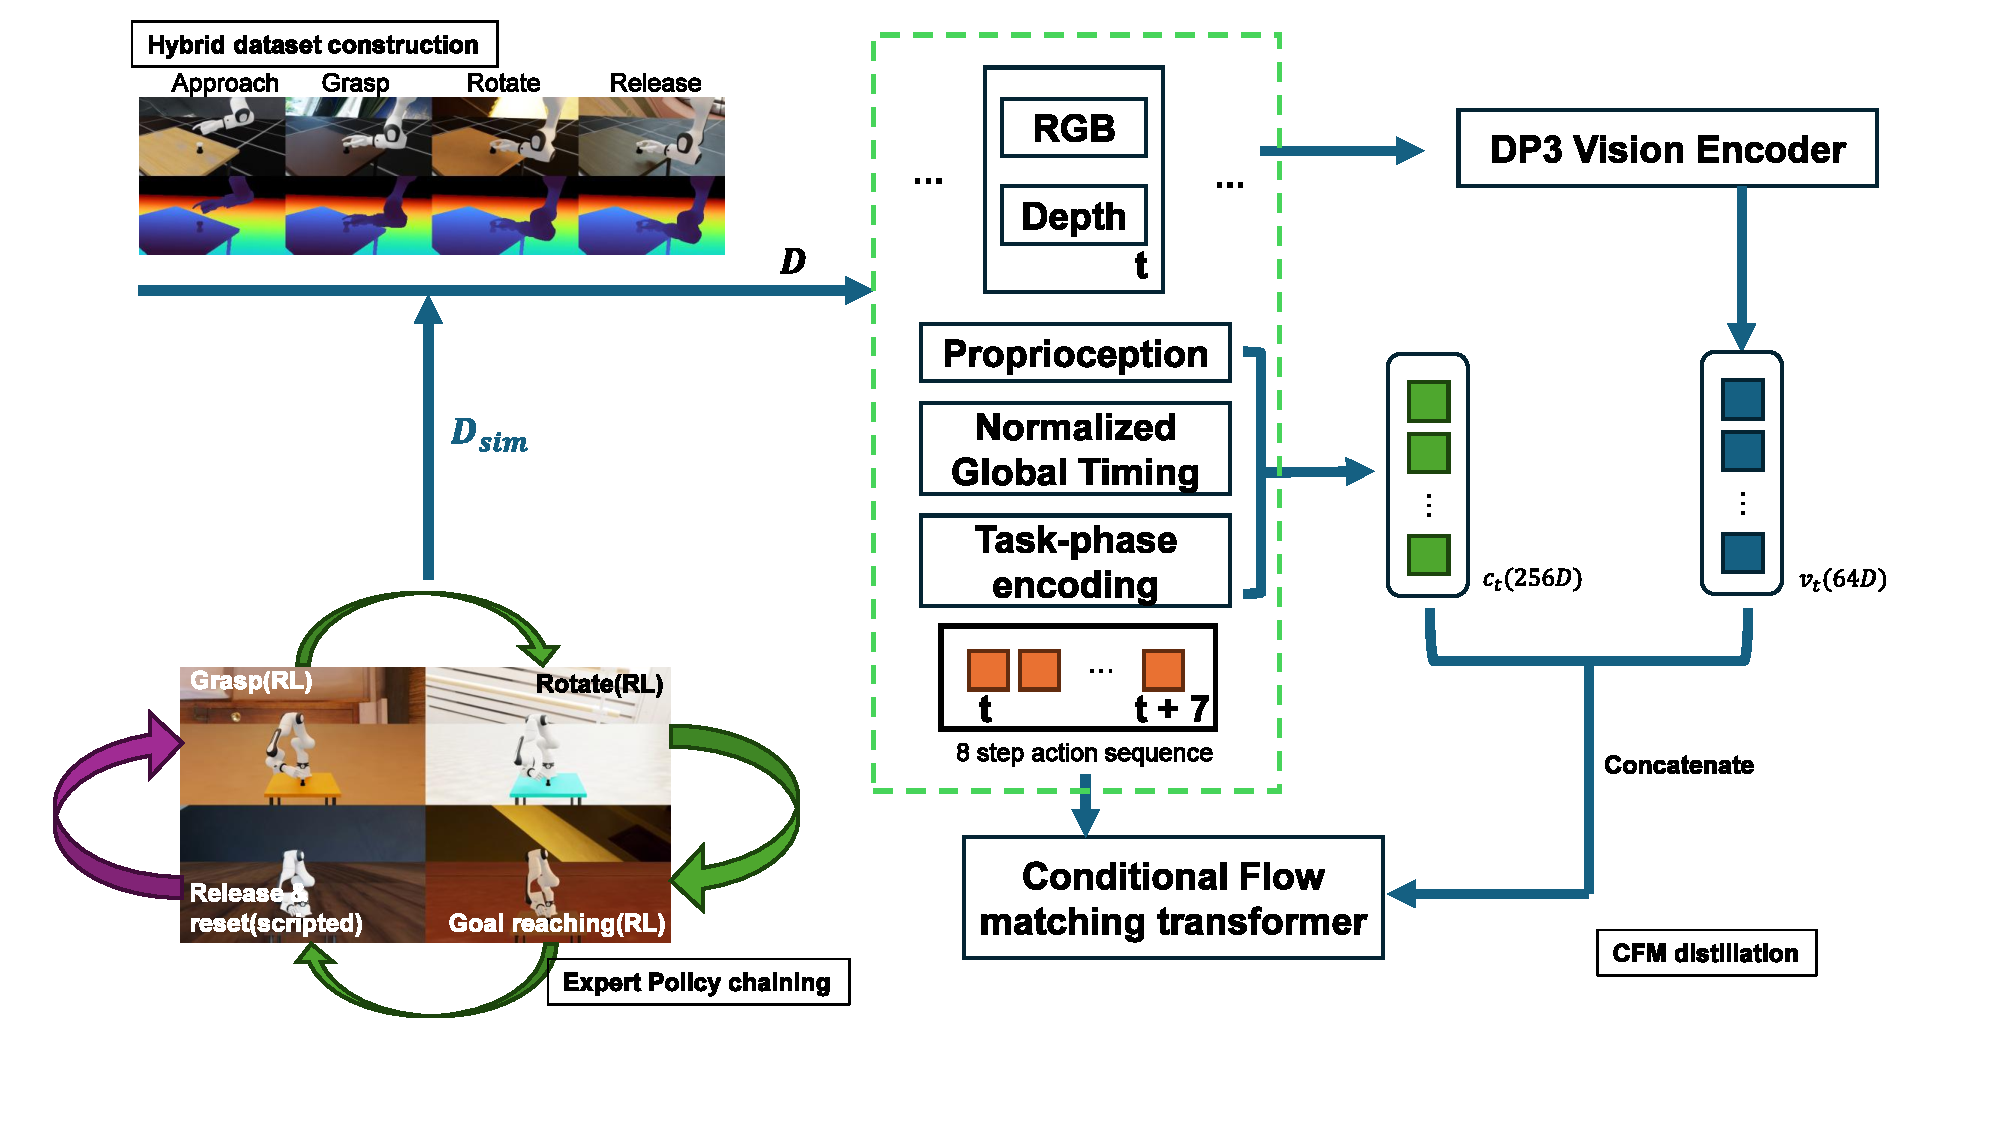
\includegraphics[width=\textwidth]{figures/mainpipeline.pdf}%
    \caption{The pipeline in detail. Left: the privileged \acs{RL} policy executes grasp, rotation, and goal reaching and a scripted controller executes release and reset. Chained in a loop, they form the hybrid teacher that generates the simulated demonstrations $\Dsim$. Right: the student encodes the aligned \acs{RGBD} observation into a 64-D point-cloud feature, fuses it with proprioception, the normalized global progress, and the process-phase encoding into a 256-D condition, and a conditional flow-matching Transformer predicts an eight-step action chunk.}%
    \label{fig:pipeline}%
\end{figure}%
% TODO(figure): mainpipeline.pdf is the project's publication figure; check that it does not show the real-world replay branch with human corrections, and edit it if it does.

\section{Problem Formulation}\label{sec:problem}

Cyclic nut threading is decomposed into the ordered phase sequence
\begin{equation}\label{eq:phases}
  \mathcal{S}=\big(\underbrace{\text{approach},\;\text{grasp},\;\text{rotate},\;\text{goal reaching}}_{\MRL:\;\piT},\;\underbrace{\text{release},\;\text{return and reset}}_{\Mscript:\;\kappa}\big).
\end{equation}
The active phase at control step $t$ is $m_t\in\Mset=\MRL\cup\Mscript$. The four phases in $\MRL$ are executed by a learned teacher policy $\piT$. The two transition phases in $\Mscript$ are executed by scripted controllers $\kappa_m$. The split is a property of the data-generation stage only: the deployed student receives neither the phase label as a switch nor separate networks per phase.

Let $K$ be the required number of cycles, $\Delta\varphi^{*}$ the desired clockwise rotation per cycle, and $\varphi_k$ the unwrapped nut angle about the bolt axis after the goal-reaching phase of cycle $k$, with $\varphi_0$ the angle at the start of the trial. The cyclic tracking error, the episodic tracking error, and the tracking cost of a trajectory $\tau$ are defined as
\begin{equation}\label{eq:errors}
  e_k=\varphi_k-\varphi_{k-1}-\Delta\varphi^{*},\qquad
  e_{\mathrm{ep}}=\varphi_K-\varphi_0-K\Delta\varphi^{*}=\sum_{k=1}^{K}e_k,\qquad
  E(\tau)=\frac{1}{K}\sum_{k=1}^{K}e_k^{2}+\beta_{E}\,e_{\mathrm{ep}}^{2}.
\end{equation}
Positive errors indicate overshoot and negative errors lag. The cost squares them so that overshoot in one cycle cannot cancel lag in another, and the weight $\beta_E$ trades accumulated drift against cycle-wise accuracy. Let $C(\tau)\in\{0,\dots,K\}$ count the cycles completed before failure or timeout and let $\Pi_{\mathcal{S}}$ denote the policies that execute the phases of $\mathcal{S}$ in order in every cycle. The research problem is to find the policy that chains all phases with maximum completion success and, among those, minimum tracking cost:
\begin{equation}\label{eq:objective}
  \Pi_{\mathrm{succ}}=\argmax_{\pi\in\Pi_{\mathcal{S}}}\;\Pr_{\tau\sim p_\pi}\!\left[C(\tau)=K\right],\qquad
  \pi^{*}=\argmin_{\pi\in\Pi_{\mathrm{succ}}}\;\E_{\tau\sim p_\pi}\!\left[E(\tau)\mid C(\tau)=K\right].
\end{equation}
Unless a study states otherwise, $K=10$ and $\Delta\varphi^{*}=60\degree$, which corresponds to one face of a hexagonal nut per cycle. The policy $\pi^{*}$ is learned from fixed hybrid-teacher demonstrations rather than by optimizing \eqref{eq:objective} on hardware, because on-robot optimization of a contact-rich cyclic task is neither safe nor sample-efficient.

The task is partially observable at deployment, so it is a \ac{POMDP}: the \ac{MDP} of Section~\ref{sec:rl-background} is extended by an observation model $O(\vec{z}_t\mid\vec{x}_t)$, and the policy acts on observations $\vec{z}_t$ instead of states~\cite{Sutton2018}. The simulator state $\vec{x}_t$ contains the nut pose, the contact state, and the controller parameters. The student observes only an aligned \acs{RGBD} image, its proprioception, and two low-dimensional conditioning signals introduced in Section~\ref{sec:student}. A single observation is then no longer sufficient to act optimally, because the information that disambiguates the state may lie in earlier observations. The teacher--student structure of the method separates the two difficulties of this \ac{POMDP}: the teacher solves the control problem with privileged state, and the student learns to perceive and to reproduce the teacher's behavior from sensor data.

\section{Simulated and Physical System}\label{sec:system}

The method is trained in simulation on a model of the physical hand--arm system and deployed on that system. This section describes the platform, the thread model that makes learning in simulation tractable, and the action contract that teacher, student, and robot share.

\subsection{Platform}\label{sec:platform}

The robot is a seven-DoF torque-controlled \ac{FR3} arm with a five-fingered Inspire RH56DFX right hand mounted on its flange (Figure~\ref{fig:platform}). The hand has twelve finger joints driven by six motors. The non-thumb fingers each have one actuated flexion joint with a mechanically coupled distal joint, and the thumb has an abduction joint and a coupled flexion chain. Only three hand degrees of freedom are commanded by the policy: thumb abduction, thumb flexion, and index flexion, which together form the pinch used for threading. The remaining fingers hold a curled posture. This restriction narrows the solution space of the dexterous hand to one grasp strategy, as difficulty~(b) of Section~\ref{sec:problem-setup} requires. The nut is threaded onto a bolt that stands on a bench in front of the robot. A fixed \acs{RGBD} camera provides the observation. Its extrinsic calibration relative to the robot base was measured on the physical cell and is reproduced in simulation.

\begin{figure}[htb]%
    \centering%
    % TODO(figure): replace the \fbox placeholders by pictures of the Franka Research 3 arm and the Inspire RH56DFX hand. Product images need a license or a citable source, which then goes into the caption.
    \begin{subfigure}[b]{0.49\textwidth}
        \centering
        \fbox{\parbox[c][5cm][c]{0.9\textwidth}{\centering\small Placeholder:\\ \acs{FR3} arm}}%
        \caption{\acs{FR3} arm.}
    \end{subfigure}\hfill
    \begin{subfigure}[b]{0.49\textwidth}
        \centering
        \fbox{\parbox[c][5cm][c]{0.9\textwidth}{\centering\small Placeholder:\\ Inspire RH56DFX right hand}}%
        \caption{Inspire RH56DFX right hand.}
    \end{subfigure}
    \caption{The robot platform. Placeholder.}%
    \label{fig:platform}%
\end{figure}%

Both teacher and student act at 15\,Hz, while the low-level controller closes its loop at the physics rate. Some design ablations of Chapter~\ref{ch:sim} were run on an earlier humanoid-arm platform that shares the thread model, the action contract, and the controller law. Simulator and timing settings are listed in Table~\ref{tab:sim-params} in the appendix.

\subsection{Simplified Thread Simulation}\label{sec:thread-model}

The thread model is the first answer to difficulty~(a) of Section~\ref{sec:problem-setup}: the skill is learned in simulation, so the simulated thread has to behave like a mating thread in each of the hundreds of parallel environments that \ac{PPO} needs. The default Isaac~Sim collision pipeline does not provide this: with \ac{SDF} mesh colliders on nut and bolt, the simulated thread contact is not accurate enough to reproduce a mating thread. A kinematic thread model also gives the policy a well-posed learning signal: with \ac{SDF} thread colliders, axial progress of the nut can be obtained by pressing it along the bolt axis, whereas a kinematic coupling makes axial progress a consequence of rotation alone, so that progress can only be earned by turning. The thread model used for teacher training therefore replaces the thread contact by a kinematic coupling, illustrated in Figure~\ref{fig:thread-model}. The nut is attached to the bolt by a passive revolute joint about the bolt axis and a coaxial, position-controlled prismatic joint. With prismatic coordinate $d_t$, unwrapped and direction-corrected revolute coordinate $\theta_t$, thread pitch $\rho$, and the index $b_k$ of the step at which the current turn started, the prismatic target is
\begin{equation}\label{eq:thread}
  d^{*}_t-d_{b_k}=-\frac{\rho}{2\pi}\left(\theta_t-\theta_{b_k}\right),
\end{equation}
so that one revolution produces one pitch of axial travel. The prismatic joint tracks $d^{*}_t$ with a stiff drive, whose finite stiffness permits small deviations from the ideal helix while the revolute--prismatic pair constrains lateral motion and keeps the nut near the commanded path. The finger--nut contact forces remain fully simulated: the policy must physically grip and turn the nut. Thread resistance is modeled on the revolute joint by a smoothed Coulomb and viscous friction torque
\begin{equation}\label{eq:friction}
  \bar{\tau}_{f,t}=-\tau_c\tanh\!\left(\frac{\omega_t}{\omega_s}\right)-c_v\,\omega_t,
\end{equation}
with revolute velocity $\omega_t$, Coulomb torque $\tau_c$, viscous coefficient $c_v$, and smoothing speed $\omega_s$. Table~\ref{tab:sim-params} lists the drive, friction, and pitch values. The model has one deliberate simplification beyond contact: the nut is initialized already engaged with the bolt. Thread engagement from a loose nut is a separate skill with a narrow entry configuration, and it is outside the scope of this thesis. The simplified contact opens a gap between the simulated and the physical thread, which the domain randomization of the teacher (Section~\ref{sec:teacher}) is meant to cover.

\begin{figure}[htb]%
    \centering%
    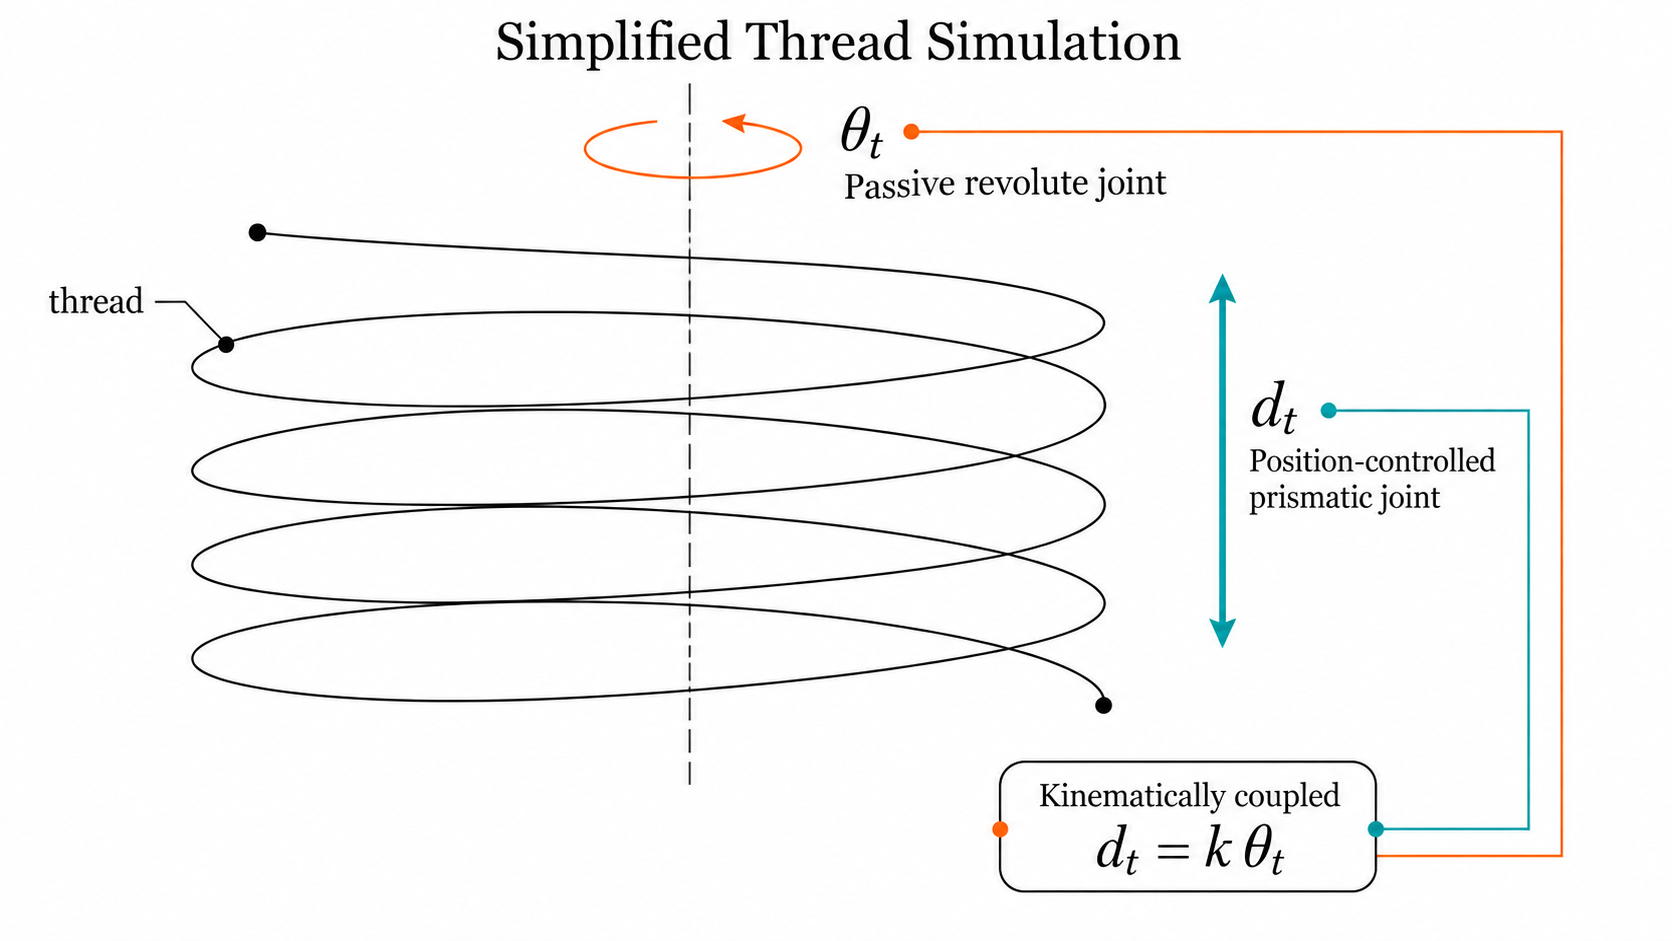
\includegraphics[width=0.62\textwidth]{figures/simplified_thread_simulation-v3.png}%
    \caption{Simplified thread simulation. A passive revolute joint $\theta_t$ about the bolt axis is kinematically coupled to a position-controlled prismatic joint $d_t$ through $d_t=k\theta_t$ with $k=-\rho/(2\pi)$, so that the nut advances by one pitch per revolution without explicit thread contacts. The finger--nut contacts remain fully simulated.}%
    \label{fig:thread-model}%
\end{figure}%

\subsection{Action Contract and Controller}\label{sec:action-contract}

The teacher acts in a 9-D action space. A fixed action decoder, described below, maps each action to a Cartesian target for the hand's grasp frame and three pinch-joint targets. The student and the scripted transitions act in the same space and use the same decoder (Section~\ref{sec:hybrid-rollout}). The grasp frame has its origin at the midpoint of the thumb and index fingertips. Its $x$ axis is the thumb-to-index direction, along which the pinch closes, and its $z$ axis is the approach direction, fixed at reset in flange coordinates. The first three components set a position offset relative to a target frame placed on the tip of the bolt. Every action component is normalized to the range from $-1$ to $1$, and the position components are scaled by 50\,mm, so the raw position action deviates by at most 50\,mm per axis from this frame. Because the target is expressed relative to the bolt, the controller draws the grasped nut toward the bolt wherever nut and robot are, and a zero action does not hold the current pose. The next three components set roll, pitch, and yaw around a neutral grasp orientation, with up to $\pm57.3\degree$ in roll and pitch and a yaw range of $[-180\degree,90\degree]$, and the last three command thumb abduction, thumb flexion, and index flexion. The raw action $\vec{a}_t$ is smoothed by an exponential moving average,
\begin{equation}\label{eq:ema}
  \tilde{\vec{a}}_t=\vec{\alpha}\odot\vec{a}_t+(1-\vec{\alpha})\odot\tilde{\vec{a}}_{t-1},
\end{equation}
with $\alpha=0.0625$ for the arm components and $3\alpha$ for the finger components, so that a single command moves the filtered action by only a small fraction of its deviation and consecutive targets stay smooth. The filtered action is decoded to a desired pose $\vec{x}^{\mathrm{des}}$, and the target passed to the controller is clipped to a bounded step from the current pose $\vec{x}$,
\begin{equation}\label{eq:steplimit}
  \vec{x}^{\mathrm{tgt}}=\vec{x}+\operatorname{clip}\left(\vec{x}^{\mathrm{des}}-\vec{x},-\vec{\delta},\vec{\delta}\right),
\end{equation}
with $\delta=0.02$\,m per axis and $0.097$\,rad per Euler angle, applied at every physics step. One command therefore cannot demand a large jump. Table~\ref{tab:controller} in the appendix lists the scales and limits.

The Cartesian target is tracked by the operational-space impedance controller of \eqref{eq:osc}. The stiffness and damping gains $\mat{K}_p$ and $\mat{K}_d$ are diagonal in world axes, with $\mat{K}_d=2\sqrt{\mat{K}_p}$ for critical damping, and the posture term uses the dynamically consistent nullspace projector of Section~\ref{sec:osc-background}. The same law runs in simulation and on the physical \ac{FR3}. The two implementations differ only in where the model quantities $\mat{J}$ and $\mat{M}$ come from and in how gravity is handled, which Table~\ref{tab:controller} in the appendix compares. The finger joints are position-controlled.

\section{Privileged Teacher Training}\label{sec:teacher}

The privileged teacher answers difficulty~(b) of Section~\ref{sec:problem-setup}. It learns to approach the nut, acquire the pinch grasp, keep it under load while turning, and stop at the target, all through the commanded hand and arm degrees of freedom of Section~\ref{sec:platform}. Because it observes privileged simulator state, it solves this control problem without having to perceive the nut (Section~\ref{sec:problem}).

The teacher for the learned phases in $\MRL$ is a recurrent policy, which keeps a hidden state $\vec{h}_t$ that integrates the history of past observations. It is trained with \ac{PPO} (Section~\ref{sec:rl-background}) in an asymmetric actor--critic~\cite{Pinto2017}, in which the critic additionally receives privileged state that exists only in the simulator and cannot be measured on the hardware. This state includes the noise-free poses of the nut and bolt, the arm joint positions, and the randomized controller gains and smoothing factor of the episode (Table~\ref{tab:teacher-obs}). The actor receives only quantities with a counterpart on the physical system, with sensor noise applied. The critic enters only through the value estimates that shape the policy gradient and is discarded after training, so the privileged state informs the update of the actor without ever being an input to it. The actor observation $\vec{z}^{\pi}_t=g_\pi(\vec{x}_t,\vec{\xi}_t)$ selects the actor-visible components of the simulator state and applies observation noise $\vec{\xi}_t$. Its 46 dimensions form four groups. The pose group holds the fingertip (grasp-frame) position relative to the bolt frame and its quaternion, the end-effector linear and angular velocity, the fingertip position relative to the held nut, and the nut quaternion. The task group holds the position and quaternion error to the current turning target and a grasp-phase flag that indicates whether the proper grasp has latched. The force group holds two fingertip forces and seven arm joint torques. The last group is the previous filtered action.

The force group mirrors the sensors of the physical system. Each fingertip channel is the force that the thumb or index pad exerts along its pad normal, computed from the total contact force on the pad regardless of the body in contact, because the physical fingertip sensors observe neither the other force components nor which body presses on them. Each torque channel is the reaction torque that the simulator measures at one arm joint, normalized by the effort limit of that joint, so that contact loads appear in it. The student observes neither channel (Section~\ref{sec:student}). Pose and force inputs are perturbed by noise that models sensor noise and calibration error (Table~\ref{tab:dr}). The critic observes clean values of the same quantities and extends them with the arm joint positions, the complete nut and bolt pose, and the sampled controller parameters, for 76 dimensions. Table~\ref{tab:teacher-obs} lists the exact components.

\begin{table}[htb]%
    \centering%
    \caption{Actor and critic observations of the single-size M24 threading teacher. Noise is applied to the actor only. Joint torques are divided by the effort limits of 87\,N\,m (joints 1--4) and 12\,N\,m (joints 5--7).}%
    \label{tab:teacher-obs}%
    \resizebox{\textwidth}{!}{%
\begin{tabular}{llcl}
        \toprule
        Input & Component & Dim & Noise (actor) \\
        \midrule
        actor (46-D) & fingertip position relative to bolt frame & 3 & $\mathcal{N}(0,0.25\,\mathrm{mm})$ per axis; bolt frame $\mathcal{N}(0,1\,\mathrm{mm})$ per reset \\
         & fingertip quaternion (WXYZ, $w$ and $z$ zeroed) & 4 & random-axis angle $\mathcal{N}(0,0.1\degree)$ \\
         & end-effector linear velocity & 3 & finite difference of noisy position \\
         & end-effector angular velocity ($x$ and $y$ zeroed) & 3 & finite difference of noisy quaternion \\
         & fingertip position relative to held nut & 3 & $\mathcal{N}(0,0.25\,\mathrm{mm})$ per axis, each body \\
         & held-nut quaternion (WXYZ) & 4 & random-axis angle $\mathcal{N}(0,0.1\degree)$ \\
         & target position error & 3 & inherits nut noise \\
         & target quaternion error (WXYZ, $w\geq0$) & 4 & inherits nut noise \\
         & grasp-phase flag & 1 & none \\
         & thumb / index flexion force & 2 & gain $U(0.8,1.2)$, offset $U(-1,1)$\,N per reset; $\mathcal{N}(0,1\,\mathrm{N})$; $\ge0$ \\
         & arm joint torques (normalized) & 7 & gain $U(0.9,1.1)$, offset $U(-0.01,0.01)$ per reset; $\mathcal{N}(0,0.005)$; in $[-1,1]$ \\
         & previous filtered action (roll, pitch masked) & 9 & none \\
        \midrule
        critic (76-D) & fingertip position, quaternion, velocities & 13 & clean \\
         & arm joint positions & 7 & clean \\
         & held-nut position, position relative to bolt, quaternion & 10 & clean \\
         & bolt position and quaternion & 7 & clean \\
         & controller proportional gains & 6 & sampled per reset \\
         & action smoothing factor & 1 & sampled per reset \\
         & thumb / index flexion force & 2 & clean \\
         & arm joint torques (normalized) & 7 & clean \\
         & position and rotation action thresholds & 6 & sampled per reset \\
         & target position, quaternion, progress & 8 & clean \\
         & previous filtered action & 9 & none \\
        \bottomrule
    \end{tabular}}
\end{table}%

The teacher is optimized with the shaped reward
\begin{equation}\label{eq:reward}
\begin{aligned}
  r_t&=\sum_{i\in\mathcal{R}} w^{r}_{i}R_{i,t}-\sum_{j\in\mathcal{P}} w^{p}_{j}P_{j,t},\\
  \mathcal{R}&=\{\text{center},\text{face},\text{grasp},\text{hold},\text{turn},\text{target}\},\\
  \mathcal{P}&=\{\text{magnitude},\Delta a,\text{align},\text{force},\text{settle},\text{wrench},\text{clear},\text{contact}\}.
\end{aligned}
\end{equation}
The reward terms follow the three phases of the learned behavior, and Table~\ref{tab:reward} in the appendix lists their exact form and weights. During approach, $R^{\mathrm{center}}$ rewards motion of the grasp center toward the nut center and $R^{\mathrm{face}}$ rewards motion of the thumb and index pads toward two designated opposing faces of the nut. Both pay only for newly achieved progress and stop paying once the grasp has latched, so repeated motion cannot accumulate reward. A proper grasp is simultaneous thumb and index contact near the designated faces with a pinch line nearly perpendicular to the nut axis. $R^{\mathrm{grasp}}$ pays a one-time bonus when the proper grasp has held for ten consecutive steps, which latches the grasp, and $R^{\mathrm{hold}}$ pays a small reward in every step in which the proper grasp holds under pad pressure. The hold reward of a complete episode is smaller than the target bonus, so holding without turning is worth less than threading. During turning, $R^{\mathrm{turn}}$ rewards newly achieved progress toward the helical target pose and pays only while the proper grasp remains live. At completion, $R^{\mathrm{target}}$ pays a bonus once, on the step at which the episode succeeds.

The penalties discourage large commands ($P^{\mathrm{magnitude}}$), abrupt action changes ($P^{\Delta a}$), misalignment of the hand frame with the nut frame ($P^{\mathrm{align}}$), excess grip force ($P^{\mathrm{force}}$), and residual rotation near the target ($P^{\mathrm{settle}}$). $P^{\mathrm{wrench}}$ prices the wrench that the thread joint transmits to the nut above small dead bands, except the torque about the bolt axis that threading requires. Its weight rises with the initial-yaw curriculum described below, so that the policy learns to thread before the force limits apply. $P^{\mathrm{clear}}$ and $P^{\mathrm{contact}}$ keep the arm off the table. In addition, the effort of the three pinch joints is limited, which bounds the grip force that the policy can apply (Table~\ref{tab:sim-params}).

Each episode samples a target turn $\theta^{*}\sim U(55\degree,65\degree)$ and builds the observed target pose at $\theta^{*}$, so the policy cannot settle on one fixed stopping angle and has to read the target from its observation. An episode succeeds when the clockwise rotation lies within $2.5\degree$ of $\theta^{*}$ under a live proper grasp for a number of consecutive steps, so overshoot fails. Success ends the episode, so the target bonus is paid once and cannot be farmed by rocking the nut across the success angle. Once the initial-yaw curriculum is complete, the required hold grows from eight to twelve steps (0.53\,s to 0.8\,s). An episode also terminates when the nut leaves the bolt, tilts, or releases the thread, when the grasp is lost after it has latched, and at the 30\,s time limit. The grasp-loss rule turns grasp retention into a hard constraint rather than a shaped term.

Robustness is obtained by domain randomization of the nut mass, the bolt friction, the controller parameters of Section~\ref{sec:action-contract}, the observations, and the initial state (Table~\ref{tab:dr}). The pose noise is small in absolute terms, because the actor's inputs are relative poses that the student will later infer from a calibrated camera. A per-episode offset of the bolt frame models calibration error and forces the teacher to close the loop on the nut rather than on the bolt frame. The initial nut rotation is randomized by an automatic curriculum that widens the yaw range from zero to $\pm30\degree$ in $5\degree$ steps whenever the success rate reaches 50\,\%, and the initial axial height of the nut is randomized as well.
\begin{table}[htb]%
    \centering%
    \caption{Domain randomization during teacher training. $U(a,b)$ denotes uniform sampling. Multiplicative factors are sampled as $1+U(0,\ell)$ or its reciprocal with equal probability. Joint torques are in units of the joint effort limits.}%
    \label{tab:dr}%
    \resizebox{\textwidth}{!}{%
    \begin{tabular}{lll}
        \toprule
        Group & Quantity & Range \\
        \midrule
        physics & nut mass offset & $U(-5,5)$\,g per reset \\
         & bolt static friction & $U(0.25,1.25)$, 128 buckets, once per environment \\
        controller & proportional gains & multiplicative, $\ell=0.41$, per axis and reset \\
         & action smoothing factor & $U(0.025,0.1)$ per reset; fingers $3\times$, capped at 1 \\
         & position / rotation threshold & multiplicative, $\ell=0.25$ / $0.29$ \\
         & dead zone & $U(0,[5,5,5,1,1,1])$ N, N\,m, resampled every 2\,s \\
        observation & fingertip and nut position & $\mathcal{N}(0,0.25\,\mathrm{mm})$ per axis and step \\
         & fingertip and nut orientation & random-axis angle $\mathcal{N}(0,0.1\degree)$ \\
         & bolt frame & $\mathcal{N}(0,1\,\mathrm{mm})$ per axis and reset \\
         & fingertip forces & gain $U(0.8,1.2)$, offset $U(-1,1)$\,N per reset; $\mathcal{N}(0,1\,\mathrm{N})$ per step; $\ge0$ \\
         & arm joint torques & gain $U(0.9,1.1)$, offset $U(-0.01,0.01)$ per reset; $\mathcal{N}(0,0.005)$ per step; in $[-1,1]$ \\
        reward & grip-force penalty threshold & $U(5,10)$\,N per reset \\
        initial state & nut yaw & curriculum $0\rightarrow\pm30\degree$ in $5\degree$ steps at 50\,\% success \\
         & nut axial height & $U(0,20)$\,mm below nominal, room for $65\degree$ reserved \\
        task & target turn $\theta^{*}$ & $U(55\degree,65\degree)$ per episode \\
        \bottomrule
    \end{tabular}}
\end{table}%

The demonstrations of this thesis are collected with this single-size M24 teacher.
% TODO(results): for the retained M24 teacher (forgeUltra force-observations branch, task config m24_threading_force_curriculum_success_term.yaml, checkpoint ...exp11-run06-success-term-2026-10-22_10-50-38/nn/last_ForgeTg2_ep_200_rew__425.6331_.pth): number of parallel environments, wall-clock time, final initial-yaw level and success-hold length (params/adr_state.yaml), and whether the run was initialized from the preceding run's checkpoint. If it was, state that here instead of implying training from scratch.
An earlier configuration of the same task, without the force group and without initial-yaw randomization, conditions one teacher on the M24, M30, and M36 nuts through a one-hot code and a round-robin assignment of sizes to environments.

\section{Hybrid Teacher and Dataset Collection}\label{sec:hybrid}

The privileged teacher turns the nut once. The hybrid teacher answers the data side of difficulty~(c) of Section~\ref{sec:problem-setup}: it chains the learned turn with scripted release and return, so that each phase is specified by the mechanism that specifies it most simply, and it rolls the chain out in simulation to produce complete multi-cycle demonstrations. This section describes the cyclic rollout, the disturbance augmentation, the vision data collection, and the dataset format.

\subsection{Cyclic Teacher Rollout in Simulation}\label{sec:hybrid-rollout}

Let $m_t\in\Mset$ denote the active phase, $\vec{x}_t$ the full simulator state, $\vec{z}^{\pi}_t$ the noisy actor observation, and $\vec{h}_t$ the actor's hidden state. During rollout the teacher is queried for its deterministic mean action $\bar{\pi}_{\mathrm{T}}(\vec{z}^{\pi}_t,\vec{h}_t)=\E_{\vec{a}\sim\piT(\cdot\mid\vec{z}^{\pi}_t,\vec{h}_t)}[\vec{a}]$. The hybrid teacher is
\begin{equation}\label{eq:hybrid}
  \piHT(\vec{x}_t,m_t)=
  \begin{cases}
    \bar{\pi}_{\mathrm{T}}(\vec{z}^{\pi}_t,\vec{h}_t), & m_t\in\MRL,\\
    \kappa_{m_t}(\vec{x}_t), & m_t\in\Mscript,
  \end{cases}
\end{equation}
where $\kappa_{m_t}$ is the scripted controller of the active transition phase. Both branches produce commands in the same filtered, bolt-relative Cartesian action space, so the recorded label is a single 9-D signal throughout the cycle. The scripted Cartesian targets are mapped back through the action decoder of Section~\ref{sec:action-contract}, and every label is the filtered target divided by a fixed per-component scale that bounds the scripted transitions to $[-1,1]$ (Table~\ref{tab:flow}). This unified label space is what makes the demonstration a coherent supervision signal for one student: at no step does the label change meaning or units.

Release is triggered when the clockwise nut rotation since the start of the cycle comes within $5\degree$ of the cycle's target turn, which lies between $55\degree$ and $65\degree$. Four Cartesian waypoints follow: the first opens the thumb and index while the arm holds its pose, and the next three retract the hand away from the nut and raise it. A final return segment brings the hand back to the initial grasp pose. The return is physically gated: it counts as complete only when the grasp frame and the hand joints are back within tolerance of their reset values, and a timeout marks the cycle as a transition failure. Table~\ref{tab:hybrid-params} in the appendix lists the thresholds and timings. While the hand is away from the nut the thread joint is held, so the nut cannot drift between cycles. On a completed return the turning reference is rebased without resetting physics. The next target turn is $60\degree$ minus the residual by which the total nut rotation misses the nearest multiple of $60\degree$, clamped to the trained range of target turns, so that a short turn is made up in the next cycle and the nut stays on the $60\degree$ grid of the hexagon. The frozen threading policy receives the nut orientation with whole $60\degree$ steps removed, which the hexagonal nut cannot distinguish, so that its observation stays within the initial-yaw range of training. The physical nut pose is not reset, so the demonstration contains the axial advance of the nut over ten cycles. The teacher population was first qualified for one period only. Repeated cycles are a property of the hybrid rollout, not of the \ac{RL} teacher alone. Figure~\ref{fig:datacollection} shows the coordinator that sequences one cycle.

Two details of the coordinator matter for the quality of the labels. First, the scripted transitions never write physics state: a transition may request that the thread joint be held while the hand is away, but it repairs nothing by teleporting the nut, so every recorded frame is a physically consistent consequence of the recorded commands. Second, the release gate is physical rather than timed: release is decided from the measured nut rotation, and the return is validated against the reset frame, so the phase labels in the recording coincide with physical events. Both properties allow the recorded phase to serve as a conditioning signal at deployment. There, the return is validated against the reset grasp pose with the same tolerances, while the release, for which the physical cell has no nut-angle sensor, is derived from the measured yaw of the grasp frame as a proxy for the nut rotation.

\begin{figure}[htb]%
    \centering%
    % Hybrid-teacher data-collection loop (cyclic coordinator).
\begin{tikzpicture}[
  font=\small,
  x=1mm, y=1mm,
  state/.style={draw, rounded corners=3pt, align=center, minimum height=12mm, inner sep=3pt, fill=white, text width=44mm},
  rl/.style={state, fill=TUMBlue!12},
  sc/.style={state, fill=TUMOrange!15},
  gate/.style={draw, diamond, aspect=2, align=center, inner sep=0.5pt, fill=white},
  arr/.style={-{Latex[length=2mm]}, thick},
]
\node[rl] (policy) at (0,0) {threading policy $\bar{\pi}_{\mathrm{T}}$:\\approach, grasp, turn, hold};
\node[gate] (relgate) at (54,0) {turn\\reached?};
\node[sc] (waypoints) at (108,0) {release:\\four waypoints, 0.7\,s each};

\node[state, fill=TUMGreen!15] (rebase) at (0,-27) {rebase turn target,\\next cycle $k{+}1$};
\node[gate] (retgate) at (54,-27) {back at\\reset?};
\node[sc] (return) at (108,-27) {return to reset pose,\\1.0\,s};

\node[state] (done) at (0,-52) {episode complete};
\node[state, fill=red!10] (fail) at (54,-52) {transition failure:\\episode rejected};

\draw[arr] (policy) -- (relgate);
\draw[arr] (relgate) -- node[above] {yes} (waypoints);
\draw[arr] (relgate.north) -- ++(0,5) -| node[pos=0.25, above] {no} (policy.north);
\draw[arr] (waypoints) -- (return);
\draw[arr] (return) -- (retgate);
\draw[arr] (retgate) -- node[above] {yes} (rebase);
\draw[arr] (retgate) -- node[right] {timeout} (fail);
\draw[arr] (rebase) -- node[left] {$k<K$} (policy);
\draw[arr] (rebase) -- node[left] {$k=K$} (done);
\end{tikzpicture}%
%
    \caption{Data-collection loop of the hybrid teacher over $K$ threading cycles. The learned policy (blue) owns approach, grasp, turn, and hold. A physical release gate on the nut rotation hands over to the scripted transitions (orange): four waypoints, which open the pinch and retreat, and the gated return. A completed return rebases the turning target and starts the next cycle, and a return that times out rejects the episode. Table~\ref{tab:hybrid-params} lists the gate thresholds. Every policy, waypoint, and return segment receives one random arm impulse, and every executed command is recorded in the common 9-D label space.}%
    \label{fig:datacollection}%
\end{figure}%

\subsection{Disturbance Augmentation}\label{sec:impulses}

Twenty demonstrations contain too little variation for a student that must recover from its own deviations. Trajectory diversity is therefore increased at collection time by applying random impulses to the arm: one impulse is applied to a random arm link shortly after the start of every policy, waypoint, and return segment of every cycle, which gives 30 impulses per ten-cycle demonstration (Table~\ref{tab:datasets}). The teacher, which is a closed-loop controller, reacts to the disturbance, and the recorded recovery is part of the label. The teacher is queried for its mean action and controls every step ($\beta=1$), so each recovery segment is the teacher's own response to the state that precedes it. Besides the impulses, the demonstrations vary through the task randomization that remains active during collection (Section~\ref{sec:dataset}). Demonstrations in which the teacher fails to complete all cycles are rejected before materialization. The retained set consists only of explicitly successful episodes.

\subsection{Vision Data Collection}\label{sec:vision-collection}

The student perceives the scene through one \acs{RGBD} camera, so the demonstrations are rendered from a simulated copy of the physical camera. The extrinsic pose of the physical camera relative to the robot base is deduced from twelve different poses of a calibrated AprilTag observed by the camera. The resulting pose and the intrinsics are used to render the simulated camera during data collection and enter the student training pipeline. The physical stream is cropped and downscaled to the $320\times180$ resolution that the simulated camera renders directly. Camera geometry and field of view therefore agree between the two domains up to calibration error. Appearance and depth quality do not, because a rendered scene has one clean appearance and a rendered depth image contains no sensor noise. Texture randomization covers the first difference at collection time, and depth augmentation covers the second during training.

Texture randomization follows DextrAH-RGB~\cite{Singh2025} and varies the appearance of the rendered scene. At every reset, each environment draws new materials for the tabletop, the nut, and the bolt, each with a random texture, roughness, and metallicity. The dome light, with its texture, orientation, and intensity, and the floor texture are shared by all parallel environments and are redrawn at a reset with a fixed probability. An environment can also replace the far and invalid pixels of the RGB image with a random background image. These pixels lie outside the crop box of the point-cloud encoder (Section~\ref{sec:student}), so the background reaches only the image-space encoders of Chapter~\ref{ch:sim}. The robot keeps its nominal appearance. Because the randomization is drawn at reset, the appearance is constant within a ten-cycle demonstration and differs between demonstrations. The offline loader cannot regenerate scene appearance from stored images, so this variation is recorded into the dataset once and reused unchanged by every student trained on it. Table~\ref{tab:datasets} lists the sampled ranges, and Figure~\ref{fig:texture-randomization} shows the resulting variation of the rendered scene.

Depth augmentation corrupts the stored metric depth images during student training. Rendered depth is exact, whereas a physical \acs{RGBD} camera returns noisy depth with missing regions, and the depth determines the position of every point that the encoder receives. The corruption is drawn anew for every training batch and acts before back-projection, so each epoch presents a different corruption of the same demonstration. It first perturbs the valid pixels with Gaussian noise whose standard deviation grows with the squared depth, adds a spatially smooth offset field, and quantizes the result. It then invalidates pixels at depth discontinuities, spatially correlated regions, and isolated pixels. Invalid pixels are rejected during back-projection, so an augmented frame yields a noisier point cloud with missing regions. The parameters in Table~\ref{tab:flow} approximate a commodity \acs{RGBD} camera qualitatively, and Figure~\ref{fig:depth-augmentation} shows their effect on a depth image. The dataset of the next subsection stores the randomized RGB images together with the noise-free depth, so the same demonstrations can be trained with or without the augmentation.
% TODO(unsure): which student is the reported one? forgeUltra exp_12 (DP3 sweep, 2026-10-27 to 10-29) used depth augmentation on, no RGB augmentation, no vision pretraining, 100 epochs, and 40 episodes, whereas Table tab:flow and Section sec:student state RGB augmentation, pretraining, and 300 epochs, and Section sec:dataset states 20 episodes.
% TODO(results): measure real depth failures, exposure, blur, and camera/control latency on the physical camera and set the simulation randomization ranges from them (forgeUltra todo.md, P2).

\begin{figure}[htb]%
    \centering%
    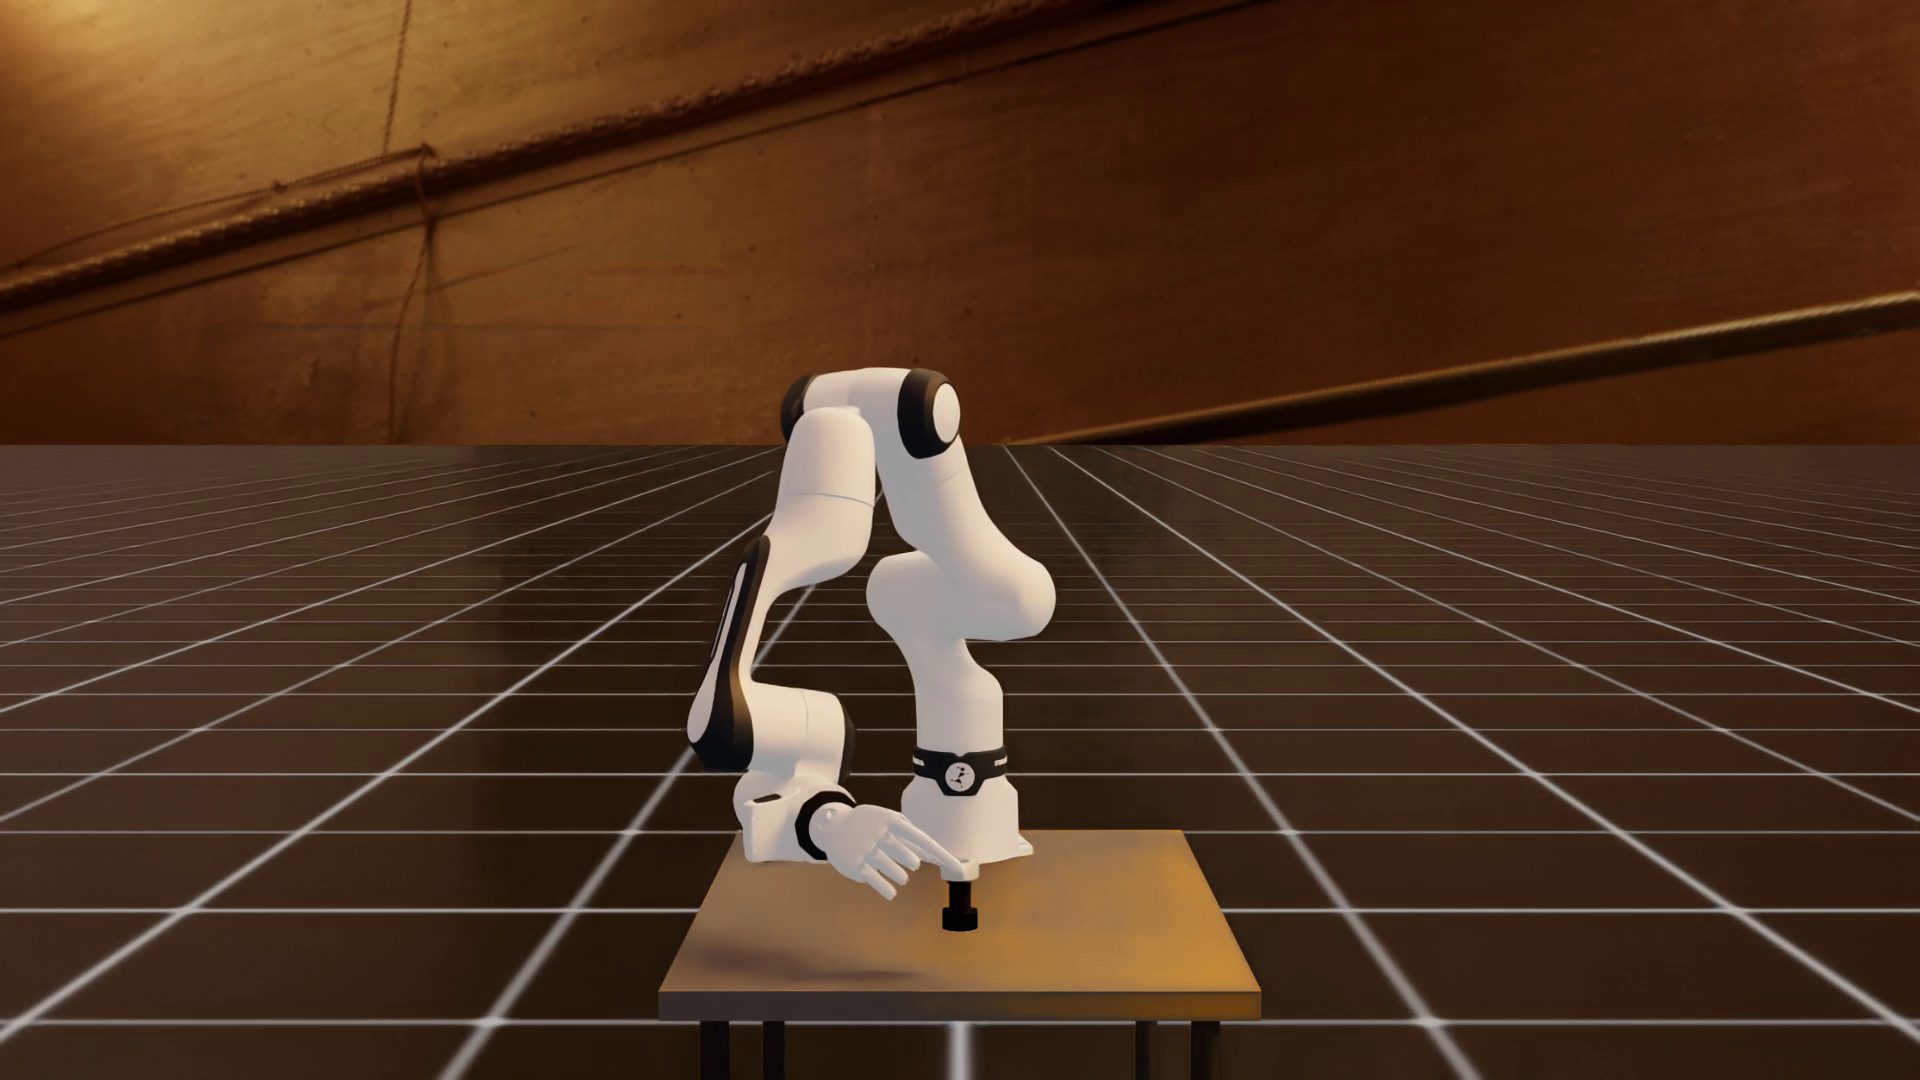
\includegraphics[width=0.45\textwidth]{figures/policy_visuals/teacher/randomization_dark.png}\hspace{2mm}%
    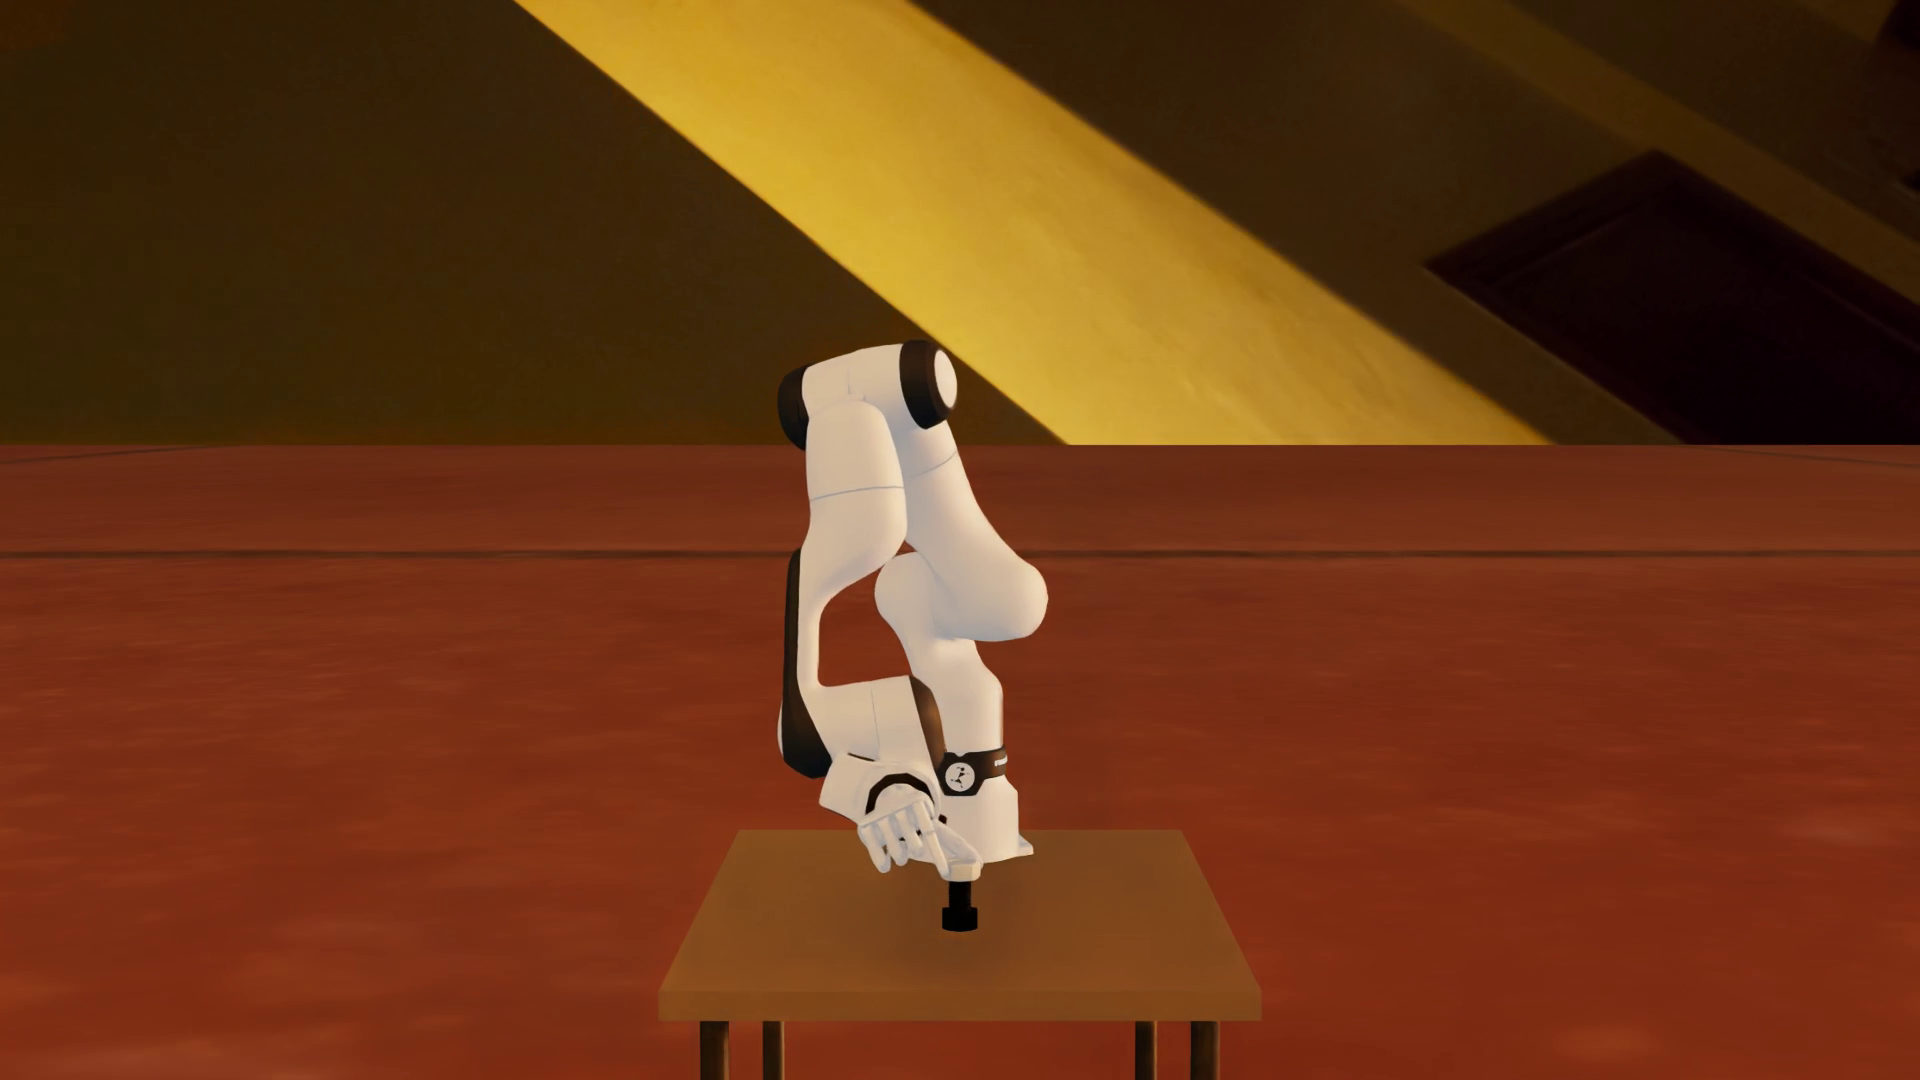
\includegraphics[width=0.45\textwidth]{figures/policy_visuals/teacher/randomization_warm.png}\\[2mm]%
    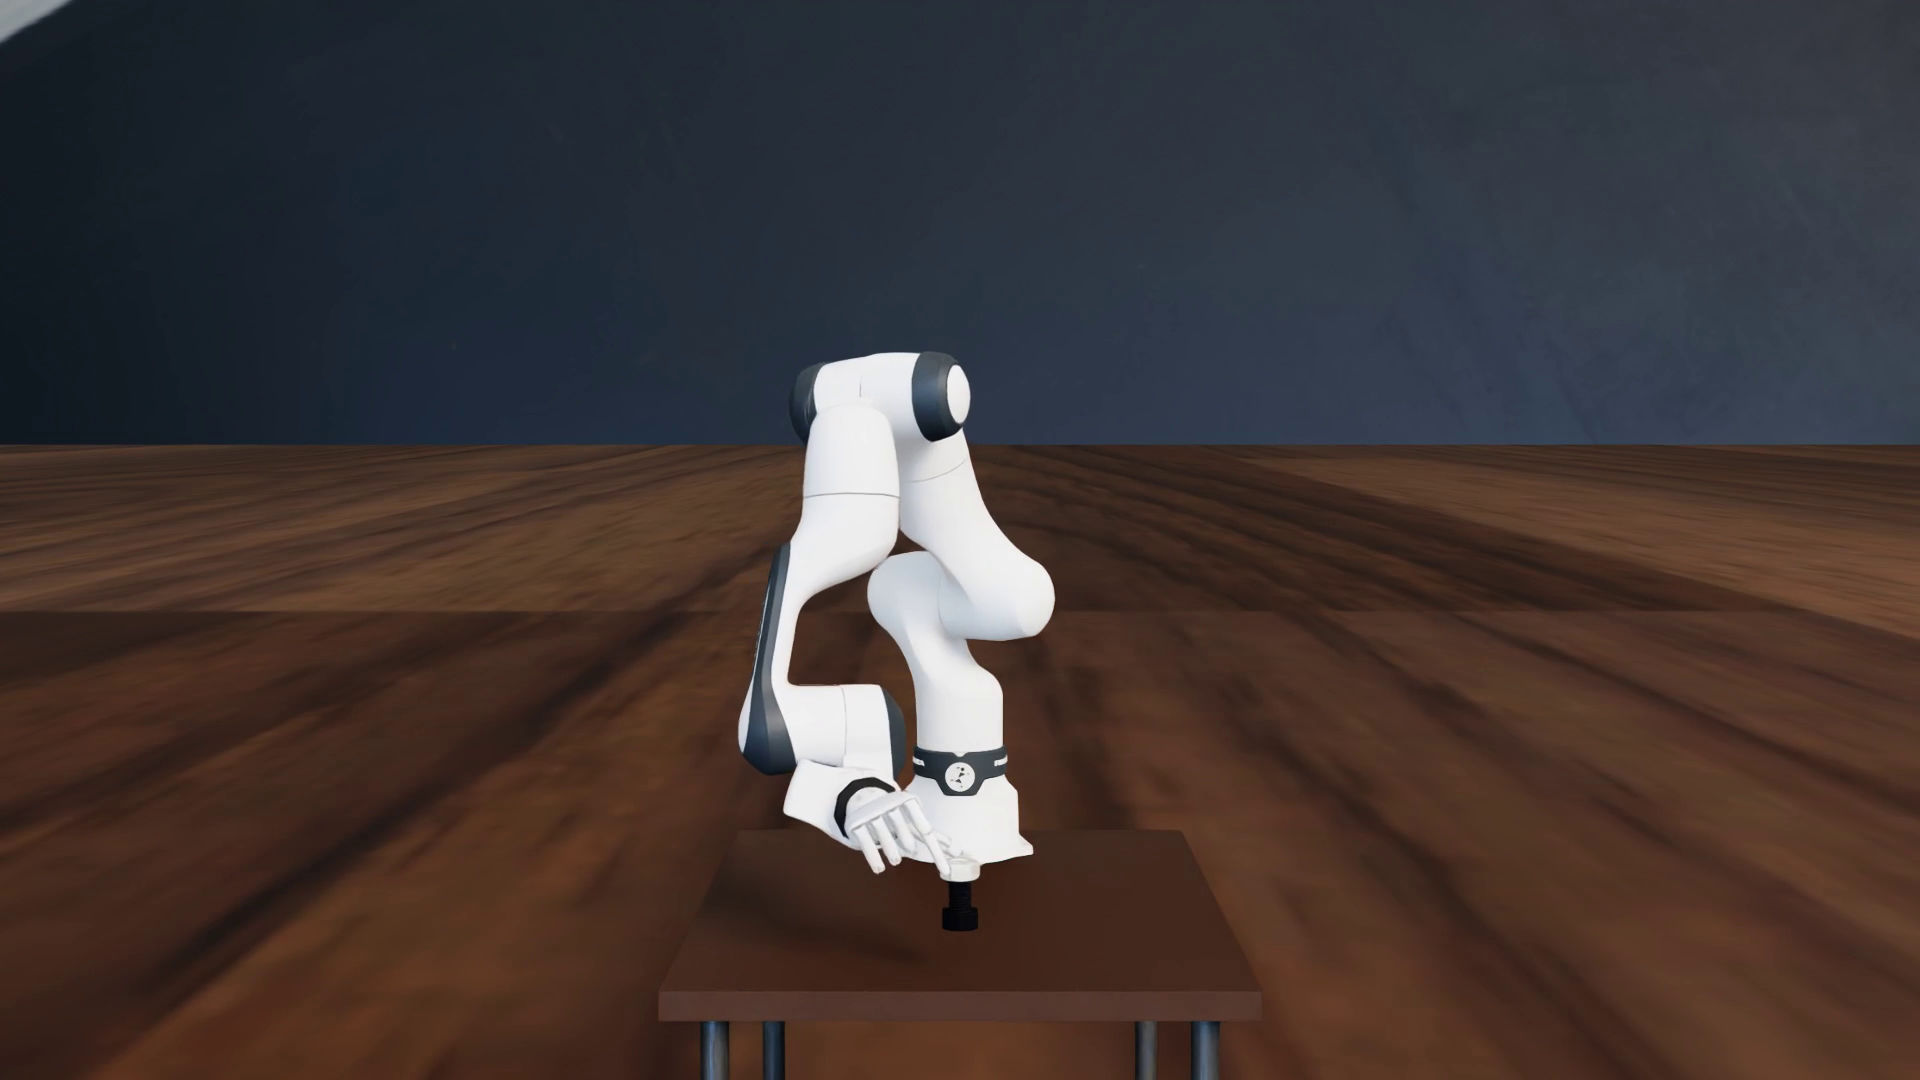
\includegraphics[width=0.45\textwidth]{figures/policy_visuals/teacher/threading_v2_lighting_texture_randomization.png}\hspace{2mm}%
    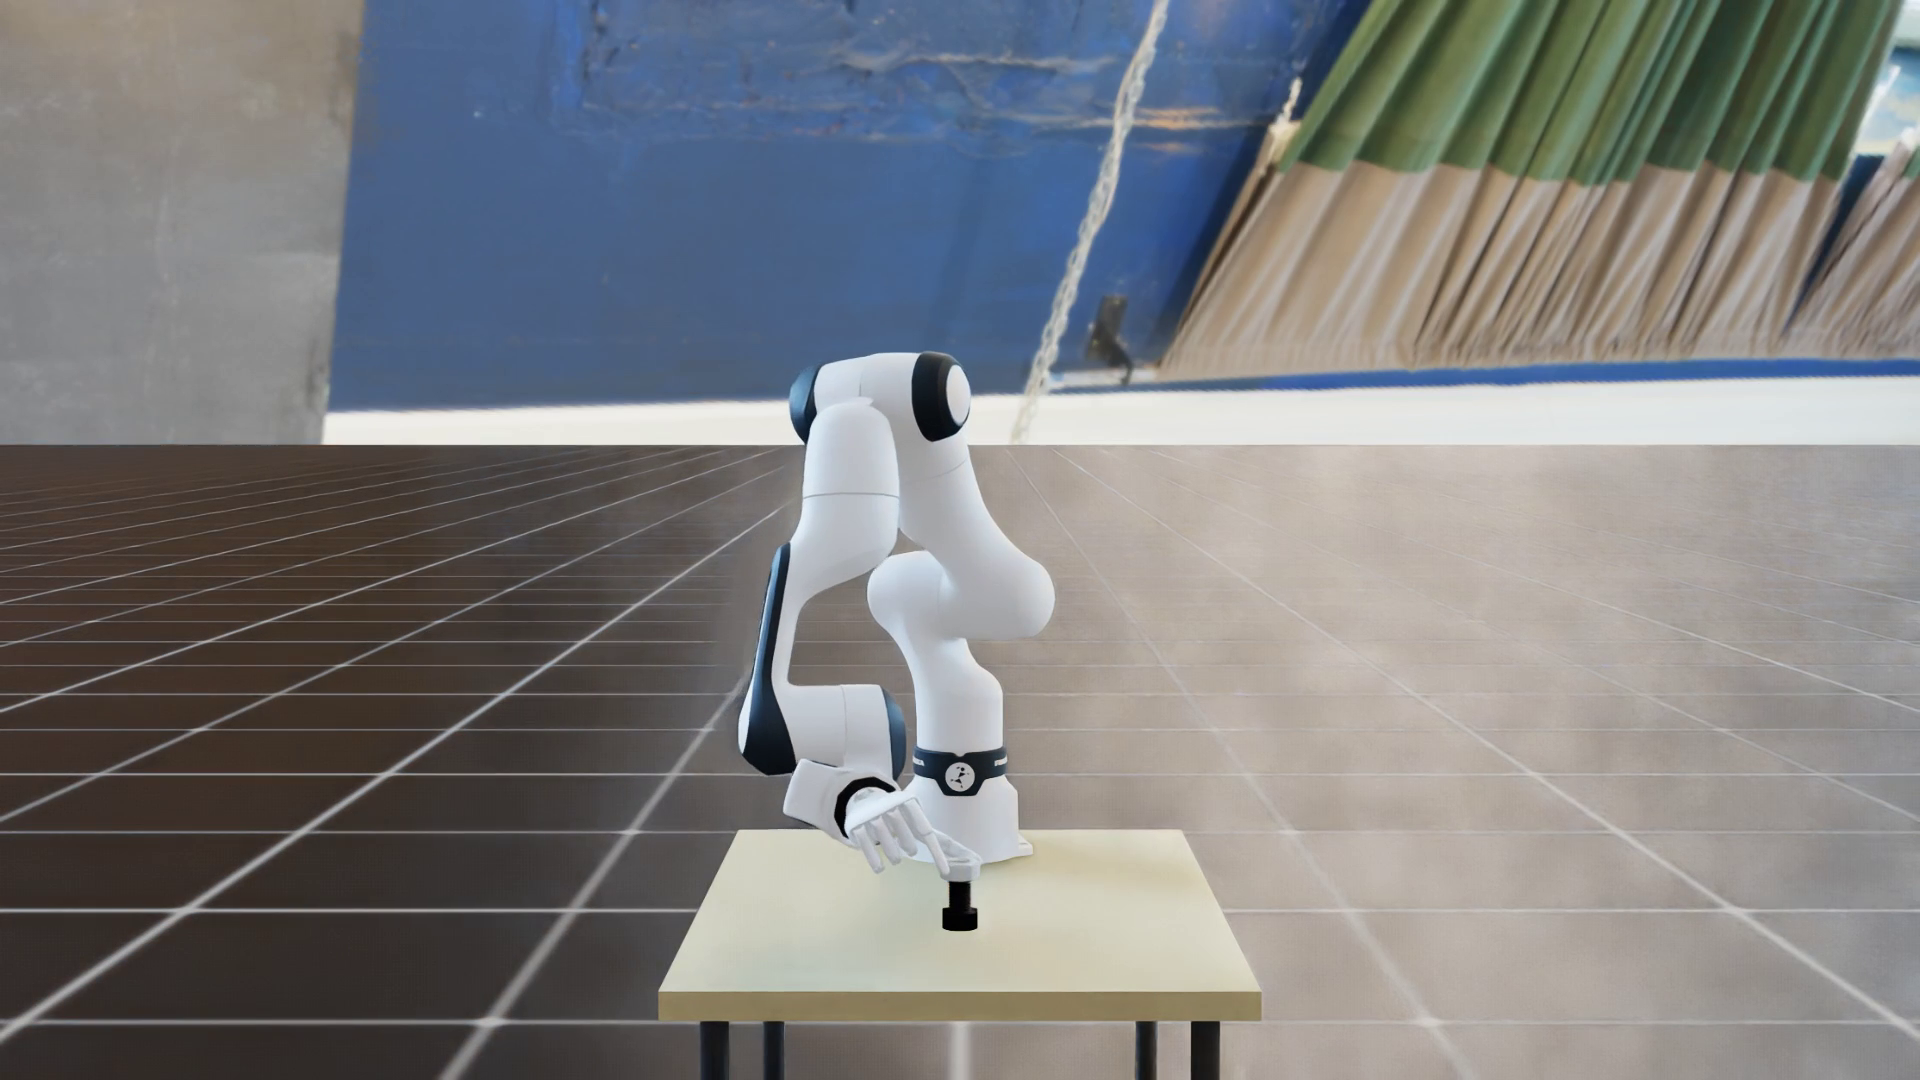
\includegraphics[width=0.45\textwidth]{figures/policy_visuals/teacher/randomization_blue.png}%
    \caption{Four draws of the texture randomization in the simulated workcell. The dome light and the textures of the floor and the tabletop change between draws, while the robot keeps its nominal appearance.}%
    \label{fig:texture-randomization}%
\end{figure}%

\begin{figure}[htb]%
    \centering%
    % TODO(figure): replace the \fbox placeholder by a noise-free depth image next to the same image after depth augmentation and additional noise.
    \fbox{\parbox[c][5cm][c]{0.9\textwidth}{\centering\small Placeholder:\\ depth augmentation and additional noise}}%
    \caption{Depth image under depth augmentation and additional noise. Placeholder.}%
    \label{fig:depth-augmentation}%
\end{figure}%

\subsection{Dataset Format}\label{sec:dataset}

The demonstrations are collected from the M24 teacher of Section~\ref{sec:teacher} with two training mechanisms switched off: success does not end the episode, and the target turn is not sampled but follows the $60\degree$ grid of Section~\ref{sec:hybrid-rollout}. Every environment starts from the nominal pose, without initial yaw and with the nut at the top of the thread, so that ten $60\degree$ turns, 1.67 revolutions or 5\,mm of axial travel on the 3\,mm pitch, fit on the bolt. All other randomization of Table~\ref{tab:dr} remains active, and an episode may last up to 200\,s.

Each demonstration is materialized as one episode file with aligned 15\,Hz samples. A sample holds the RGB and metric depth images at $320\times180$ pixels, the 29-D proprioception, the executed 9-D command, the active process phase, the nut pose for privileged ablations and auxiliary supervision, and the timestamp, from which the normalized task progress is derived. Action chunks never span a reset, phase boundaries are retained so that the student learns the transitions, and terminal chunks are padded with the final command so that the last observations of an episode remain conditioning states. The retained M24 dataset contains 20 successful ten-cycle demonstrations collected from 32 parallel environments, with \tbd{} frames in total (Table~\ref{tab:datasets}).
% TODO(results): frame count, number of candidate episodes and rejections, and the DP3 valid-point audit of the M24 ten-cycle collection (recipe m24_v2_run06_success_term_yaw0_10cycle_sequential_dual_supervision_v1, forgeUltra commit 304d4d9 reports 20/20 trajectories and 26 successful episodes).

\section{Student Policy Distillation by Conditional Flow Matching}\label{sec:distillation}

The student answers the deployment side of difficulty~(c) of Section~\ref{sec:problem-setup}. The hybrid teacher cannot be deployed, because both its learned policy and its scripted controllers act on privileged simulator state \eqref{eq:hybrid}. The student replaces it with one visuomotor policy that executes every phase of every cycle from sensor data, without a phase switch or separate networks. RQ1 asks whether this unified student sustains consecutive cycles better than a single-cycle policy invoked repeatedly. RQ2 asks which student design distills the demonstrations best. The alternative encoders of Section~\ref{sec:student} and the regression baselines of Section~\ref{sec:baselines} are its comparisons.

\subsection{From Behavior Cloning to Online Distillation for Cyclic Tasks}\label{sec:why-dagger}

Student learning is posed as supervised imitation from the fixed dataset $\Dset$. Section~\ref{sec:il-background} explained why plain behavior cloning is fragile over long horizons: the student is evaluated on the states that its own errors produce. For cyclic threading the mechanism is concrete. A student that grasps a millimeter too high applies a slightly different torque, the nut advances a little less, and after a few cycles the fingers close on the edge of the nut instead of on its faces. Three measures counter this compounding in the present method, and they are complementary. First, the demonstrations themselves contain recoveries, because the closed-loop teacher was disturbed by impulses during collection. The student thus sees off-nominal states with correct labels, which is the effect \ac{DAgger} produces by querying the expert on student-visited states, obtained here without an expert that can be queried at arbitrary states. Second, the student predicts action chunks and executes a temporal ensemble of overlapping chunks, which filters the single-step noise that would otherwise be amplified by the controller. Third, where a queryable expert exists, in simulation, a flow-matching student of the same architecture can be trained online with the hybrid teacher labeling the states that the student visits. This online variant is described in Section~\ref{sec:online-flow}. Its comparison with the offline variant in Chapter~\ref{ch:sim} is pending. The deployed student is trained offline on $\Dset$: the ten-cycle dataset is rendered once under visual randomization and shared by the full method and ablations (b) to (d) of Chapter~\ref{ch:sim}. Online \ac{DAgger} serves as a comparison in simulation.

\subsection{Conditional Flow Matching}\label{sec:flow-matching}

The action head of the student is a conditional flow-matching model~\cite{Lipman2023,Lipman2024}, whose principle Section~\ref{sec:generative-background} introduced. This section states what the head is trained to generate and which signals it is conditioned on.

The head generates action chunks. Its training target is the demonstrated chunk of the next $H$ commands, $\Uc^{D}_t=[\act_t,\dots,\act_{t+H-1}]\in\R^{H\times9}$. The chunk is conditioned on the student observation $\obs_t=(\vec{O}^{\mathrm{RGBD}}_t,\vec{s}_t,p_t,\vec{e}^{m}_t)$. The \acs{RGBD} image $\vec{O}^{\mathrm{RGBD}}_t$ of the head camera shows the hand, the nut, and the bolt. The proprioception $\vec{s}_t$ holds the joint positions, the joint velocities, and the previous action. The normalized task progress $p_t\in[0,1]$ tells the student how far into the trial it is, and the process-phase encoding $\vec{e}^{m}_t$ marks whether the policy, the release waypoints, or the return is active. The network of Section~\ref{sec:student} encodes these signals into one condition vector $\cond_t$, which takes the place of $\obs$ in \eqref{eq:fm-loss}. Training applies the straight-line construction of \eqref{eq:fm-line} to whole chunks:
\begin{equation}\label{eq:student-objective}
  \theta^{*}=\argmin_\theta\;\E\left\|\vfield\!\left(\Uc^{\lambda}_t,\lambda\mid\cond_t\right)-\dot{\Uc}^{\lambda}_t\right\|_2^{2},\qquad
  \Uc^{\lambda}_t=(1-\lambda)\Uc^{0}_t+\lambda\Uc^{D}_t,\quad
  \dot{\Uc}^{\lambda}_t=\Uc^{D}_t-\Uc^{0}_t,
\end{equation}
where the expectation is over $(\obs_t,\Uc^{D}_t)\sim\Dset$, a Gaussian chunk $\Uc^{0}_t\sim\mathcal{N}(\vec{0},\mat{I})$ of the same shape, and $\lambda\sim U[0,1]$. At run time, the student draws a Gaussian chunk $\Uc^{0}$ and follows the learned field with $N$ explicit Euler steps, $\Uc^{\lambda+1/N}=\Uc^{\lambda}+\frac{1}{N}\vfield(\Uc^{\lambda},\lambda\mid\cond_t)$, with $N=16$ in simulation (Table~\ref{tab:flow} lists the deployment setting). The condition $\cond_t$ is computed once per chunk, so the image is encoded once and each Euler step evaluates only the Transformer of Section~\ref{sec:student}.

A generative head is used because the demonstrations are multimodal. The teacher's recoveries after impulses depend on state that the observation does not fully resolve, so near-identical observations can carry the nominal action in one demonstration and a recovery in another. A regression head averages such labels, whereas the flow head samples one of them (Section~\ref{sec:generative-background}). Among generative heads, flow matching is chosen over diffusion because it trains on a plain regression target without a noise schedule and samples in a few deterministic integration steps. The deterministic regression baselines of Section~\ref{sec:baselines} test whether the generative head pays off.

\subsection{Student Architecture}\label{sec:student}

Figure~\ref{fig:student} shows the student. It consists of a vision encoder, a proprioception encoder, a fusion and conditioning stage, and the velocity network.

\begin{figure}[htb]%
    \centering%
    % Student architecture block diagram (styled after figures/Distillation-Pipeline.png).
\begin{tikzpicture}[
  font=\scriptsize,
  x=1mm, y=1mm,
  box/.style={draw, rounded corners=2pt, align=center, minimum height=7mm, inner sep=1.5pt, fill=white},
  inp/.style={box, rounded corners=0pt, draw=TUMGray2, fill=TUMGray3!70, text width=21mm},
  lrn/.style={box, draw=TUMDiagGreen2, fill=TUMDiagGreen2!15, text width=19mm},
  op/.style={box, text width=19mm},
  grp/.style={dashed, line width=1pt, rounded corners=1pt},
  ttl/.style={font=\footnotesize\bfseries, anchor=south west, inner sep=1pt},
  arr/.style={-{Latex[length=1.8mm]}, semithick},
  pics/fvec/.style={code={
    \draw[rounded corners=1.5pt, fill=white] (-2.2,-6.5) rectangle (2.2,6.5);
    \foreach \yy in {4.2,1.4,-4.2} \fill[#1, rounded corners=0.4pt] (-1.3,\yy-1) rectangle (1.3,\yy+1);
    \foreach \yy in {-0.8,-1.7,-2.6} \fill (0,\yy) circle (0.22);
    \coordinate (-n) at (0,6.5); \coordinate (-s) at (0,-6.5);
    \coordinate (-e) at (2.2,0); \coordinate (-w) at (-2.2,0);
  }},
]
% ---------------- vision encoding ----------------
\node[inner sep=0pt] (rgb)   at (13,15) {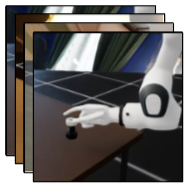
\includegraphics[height=12mm]{figures/student/rgb_stack.png}};
\node[inner sep=0pt] (depth) at (13,2)  {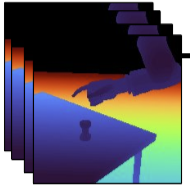
\includegraphics[height=12mm]{figures/student/depth_stack.png}};
\node at (3.5,15) {RGB};
\node at (3.5,2)  {D};
\node[inner sep=0pt] at (13,-6.5) {aligned, $320\times180$};
\node[inner sep=0pt] (pcimg) at (40,0) {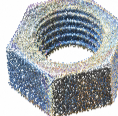
\includegraphics[height=12mm]{figures/student/nut_pointcloud.png}};
\node[above=1mm of pcimg, align=center, inner sep=0pt] {back-projection, crop,\\4096 points};
\node[lrn] (dp3)  at (64.5,0) {PointNet\\64--128--256,\\max pooling};
\pic (v) at (87.5,0) {fvec=TUMBlue3};
\node[anchor=west, align=left, inner sep=0pt] at (91,0) {$\vec{v}_t$\\64-D};
\node[lrn, dashed, text width=32mm] (aux) at (84,14) {aux.\ head 64--128--3:\\nut position (training only)};
\draw[arr] (rgb.east) -- ++(7,0) |- ([yshift=2mm]pcimg.west);
\draw[arr] (depth.east) -- ++(3,0) |- ([yshift=-2mm]pcimg.west);
\draw[arr] (pcimg) -- (dp3);
\draw[arr] (dp3) -- (v-w);
\draw[arr, dashed] (v-n) -- (v-n |- aux.south);

% ---------------- state and task encoding ----------------
\node[inp] (prop)  at (13.5,-28) {proprioception\\$\vec{s}_t$ (29-D)};
\node[inp] (phase) at (13.5,-40) {process phase\\$\vec{e}^{m}_t$ (one-hot, 3)};
\node[inp] (prog)  at (13.5,-52) {progress\\$p_t\in[0,1]$};
\node[lrn] (pmlp)  at (40,-28) {MLP\\128--128, ELU};
\node[lrn] (eemb)  at (40,-40) {MLP\\3--256--256};
\node[lrn] (pemb)  at (40,-52) {MLP\\1--256--256};
\pic (s) at (62,-28) {fvec=TUMDiagGreen2!60};
\node[below=0.5mm of s-s, inner sep=0pt] {128-D};
\node[lrn, text width=24mm] (fuse) at (87.5,-28) {concat $[\vec{v}_t\,\|\,\cdot\,]$\\linear $\rightarrow$ 256, ELU};
\node[op, circle, text width=, minimum height=0pt, inner sep=0.3pt, font=\footnotesize] (sum) at (87.5,-46) {$+$};
\pic (c) at (100,-46) {fvec=TUMDiagGreen2!60};
\node[above=0.5mm of c-n, inner sep=0pt] {$\cond_t$};
\node[below=0.5mm of c-s, inner sep=0pt] {256-D};
\draw[arr] (prop) -- (pmlp);
\draw[arr] (phase) -- (eemb);
\draw[arr] (prog) -- (pemb);
\draw[arr] (pmlp) -- (s-w);
\draw[arr] (s-e) -- (fuse);
\draw[arr] (v-s) -- (fuse);
\draw[arr] (fuse) -- (sum);
\draw[arr] (eemb.east) -- (79,-40) |- (sum.west);
\draw[arr] (pemb.east) -| (sum.south);
\draw[arr] (sum) -- (c-w);

% ---------------- flow-matching action head ----------------
\node[inp, text width=15mm, anchor=north, minimum height=12mm] (time)  at (120.5,21) {flow time $\lambda$\\sinusoidal\\(64)};
\node[inp, text width=15mm, anchor=north, minimum height=12mm] (noise) at (141.5,21) {noisy chunk\\$\Uc^{\lambda}$\\$8\times9$};
\node[lrn, text width=30mm] (tf) at (131.5,-7) {trajectory Transformer,\\non-causal\\$[\cond_t,\lambda,\act^{\lambda}_{1},\dots,\act^{\lambda}_{8}]$\\4 layers, 8 heads\\width 512, FF 2048};
\node[op, text width=26mm] (vel) at (131.5,-26) {velocity $\vfield\in\R^{8\times9}$};
\node[op, text width=26mm] (ode) at (131.5,-38) {Euler ODE, $N$ steps\\$\rightarrow$ chunk $\Uc_t$};
\node[op, text width=26mm] (ens) at (131.5,-50) {temporal ensemble\\$0.5^{k}$, clip $[-1,1]$};
\draw[arr] (time.south) -- (time.south |- tf.north);
\draw[arr] (noise.south) -- (noise.south |- tf.north);
\draw[arr] (c-e) -- (107,-46) |- (tf.west);
\draw[arr] (tf) -- (vel);
\draw[arr] (vel) -- (ode);
\draw[arr] (ode) -- (ens);
\draw[arr, dashed] (ode.east) -- (152,-38) |- (noise.east);
\node[rotate=90, inner sep=0pt] at (149,-28) {$N$ iterations};

% ---------------- groups ----------------
\draw[grp, TUMBlue]            (0,-9)      rectangle (105,23);
\draw[grp, TUMDiagRed1!70]     (0,-60)     rectangle (105,-17);
\draw[grp, TUMOrange!70!black] (109.5,-60) rectangle (154.5,23);
\node[ttl] at (0,23)     {Vision encoding};
\node[ttl] at (0,-17)    {State and task encoding};
\node[ttl] at (109.5,23) {Flow-matching head};
\end{tikzpicture}%
%
    \caption{Student architecture. The aligned \acs{RGBD} observation is back-projected into a point cloud and encoded into a 64-D visual feature. The 29-D proprioception is encoded by an \acs{MLP}. Late fusion concatenates the two with the visual feature first and projects to the 256-D condition, to which learned embeddings of the global trajectory progress and of the process phase are added. A non-causal trajectory Transformer predicts the flow velocity of all eight action tokens given the condition token and a sinusoidal embedding of the flow time. An auxiliary head regresses the nut position from the visual feature during training.}%
    \label{fig:student}%
\end{figure}%

\paragraph{Observation encoding and late fusion.}
Following DextrAH-RGB~\cite{Singh2025}, the visual and proprioceptive streams are encoded separately and fused by concatenation, with the visual feature placed before the encoded proprioception. The 29-D proprioception $\vec{s}_t$, consisting of the ten controlled joint positions, the ten joint velocities, and the previous filtered 9-D action, is encoded by an \acs{MLP}, and the concatenation of the 64-D visual feature and the proprioceptive feature is projected to the 256-D condition. In the privileged ablations of Chapter~\ref{ch:sim} the vision encoder is replaced by the identity and the nut position (3-D) or the nut position with its canonical axis-angle orientation (6-D) is appended to the proprioception instead. In the ablation that removes the hand velocities, the three pinch-joint velocities are dropped and the proprioception becomes 26-D.
% TODO(unsure): forgeUltra documents 29-D as the baseline, but its recommended DP3 command and the deployed 2026-10-13 checkpoint use --hand-velocity-observation omitted (26-D). Confirm which width the student now training on the M24 ten-cycle dataset uses; if 26-D, make it the method here, in Figure fig:student, and in Table tab:flow.

\paragraph{Vision encoder.}
The retained encoder follows \ac{DP3}~\cite{Ze2024}. The depth image is back-projected through the calibrated intrinsics into camera-frame points. Points outside a fixed crop box around the workspace or outside the valid depth range are rejected, and the remaining points are normalized by fixed workspace constants and carry the color of their pixel. From the valid points, 4096 are sampled, randomly during training and with a fixed priority at evaluation. A compact PointNet with pointwise layers and global max pooling yields the 64-D visual feature $\vec{v}_t$. The encoder has no generic pretrained backbone. It is pretrained on the task scene and then fine-tuned inside the student, as described below. The alternative encoders compared in Chapter~\ref{ch:sim} share the same 64-D interface and the same $320\times180$ \acs{RGBD} input. An image-space encoder, ablation (b) of Chapter~\ref{ch:sim}, applies an ImageNet-pretrained ResNet-18 trunk to RGB, depth, and a validity mask, adds an embedding of the camera-frame point coordinates, and pools the resulting tokens by attention. An Adapt3R-style encoder~\cite{Wilcox2025} lifts frozen ResNet-18 features to 3D through the depth map, expresses them in the grasp frame, and pools them by attention.

\paragraph{Encoder pretraining in parallel scenes and fine-tuning.}
The point-cloud encoder is first trained alone, on a pose-regression task in parallel simulated scenes, and then fine-tuned end to end inside the student. The pretraining scenes contain the workcell table, the nut and bolt, and the calibrated camera, but no robot. In every scene a free-floating nut follows a random six-DoF path through the visible workspace, and the rendered \acs{RGBD} frames are consumed immediately by the encoder and a pose decoder. The decoder predicts the camera-frame nut position and orientation with a loss that treats the six $60\degree$ rotations of the hexagonal nut as equivalent. Only the encoder weights are transferred to the student, and the pose decoder is discarded. All encoder parameters remain trainable and are optimized jointly with the flow head, so the representation adapts to the hybrid-teacher scenes and to the action objective. Table~\ref{tab:flow} lists the pretraining budget and its validation errors.
% TODO(unsure): confirm that the student now training on the M24 ten-cycle dataset is initialized from the same pretraining checkpoint (fr3_d415_nut_sweep_20260910T152223_calibration/nn/best.pt) with the encoder left trainable.

\paragraph{Conditioning on progress and phase.}
Two low-dimensional conditions are added to the 256-D condition through separate learned embeddings. The global trajectory progress $p_t\in[0,1]$ maps the first timestamp of each demonstration to 0 and the last to 1. At deployment it advances with elapsed time from the start of the trial, normalized by the median demonstration duration stored in the checkpoint, and is clamped to 1 afterwards. It is a monotonic clock for the complete behavior and nothing more: it is not a teacher-stage selector, it is not periodic, and it does not encode the cycle index. It tells the student how far into a nominally timed trial it is, which disambiguates, for instance, the first and the last approach of a trial that otherwise look alike. The process-phase encoding $\vec{e}^{m}_t$ is a three-way one-hot over the policy-controlled phases, the release waypoints, and the return. During training it is derived from the recorded phase labels, and during evaluation it is published by the cyclic coordinator, in simulation from the physical events of Section~\ref{sec:hybrid-rollout} and on the robot from the release proxy and return gate, so that a cycle that takes longer than nominal cannot select the wrong phase. The phase encoding is a synchronization aid: it does not switch networks or action contracts, and the student predicts the transition actions itself.
% TODO(unsure): an earlier description of the method lists a one-hot over all six phases of (1); the code derives a three-way one-hot (policy, release waypoints, return). The text follows the code.

\paragraph{Velocity network.}
The velocity field is a non-causal trajectory Transformer. The noisy chunk $\Uc^{\lambda}$ is split into $H=8$ action tokens of dimension 9. A condition token embeds $\cond_t$, and a time token embeds the flow time $\lambda$ through a sinusoidal encoding. Learned positional embeddings mark the token slots and carry no absolute time. The Transformer applies full self-attention over all tokens, so that every step may attend to the whole noisy chunk when predicting its velocity, and a linear output layer maps each action token to its 9-D velocity. The model keeps an exponential moving average of its parameters, and inference uses the averaged weights. An auxiliary head on the visual feature regresses the nut position. It regularizes the visual feature toward spatially meaningful content and is discarded at deployment. Table~\ref{tab:flow} in the appendix lists the network sizes and the training hyperparameters.

\paragraph{Action chunking and execution.}
With $H=8$ and 15\,Hz, one chunk covers 0.53\,s, and its first action is the command that acts on the observed state. At deployment the student replans at every control step, and the command sent to the controller is a temporal ensemble of all still-valid proposals for the current tick with weights $0.5^{k}$ for a proposal of age $k$. A decay of zero recovers strict first-action execution. The ensemble operates in action space and is distinct from the parameter-space \acs{EMA}. The executed 9-D action is clipped to $[-1,1]$, decoded to the filtered Cartesian target, and passed to the controller of Section~\ref{sec:action-contract}. Because the label scale is fixed, no action statistics are learned.
% TODO(results): measure student inference latency (image encoding + 16 ODE steps) on the deployment machine and report it in Chapter 5.

\subsection{Offline Training}\label{sec:offline-flow}

Algorithm~\ref{alg:offline} summarizes offline distillation. The dataset consists of the simulated hybrid-teacher rollouts, windows of $H$ consecutive commands are built from each episode without crossing episode boundaries, and the velocity field is trained with \eqref{eq:student-objective} while an \acs{EMA} copy of the parameters is maintained.

\begin{algorithm}[htb]%
    \caption{Offline flow distillation}\label{alg:offline}
    \begin{algorithmic}[1]
        \Require hybrid teacher $\piHT$, horizon $H$
        \State Collect simulated rollouts $\Dsim$ with $\piHT$ under random arm impulses and visual domain randomization
        \State Form $H$-step chunks from $\Dset=\Dsim$, masking resets and padding terminal chunks
        \Repeat
            \State Sample $(\obs_t,\Uc^{D}_t)\sim\Dset$, $\Uc^{0}_t\sim\mathcal{N}(\vec{0},\mat{I})$, $\lambda\sim U[0,1]$
            \State Encode the point cloud and fuse it with proprioception, progress, and phase to obtain $\cond_t$
            \State Update $\theta$ by one gradient step on \eqref{eq:student-objective} plus the auxiliary nut-position loss
            \State Update \acs{EMA} parameters $\bar{\theta}\leftarrow\alpha\bar{\theta}+(1-\alpha)\theta$
        \Until{convergence}
        \State \Return student velocity field $\vec{v}_{\bar{\theta}}$
    \end{algorithmic}
\end{algorithm}%

\subsection{Online \acs{DAgger} with a Flow-Matching Head}\label{sec:online-flow}

The online variant replaces the fixed dataset by live teacher labels. The simulator is driven by a mixture of teacher and student control with teacher probability $\beta$, the hybrid teacher labels every visited state with its 9-D command, and the flow head is trained on the labels as they arrive. The online student differs from the offline student in its inputs and targets: it uses the two-branch \acs{RGBD} encoder instead of the point-cloud encoder, it supervises the teacher's normalized native action instead of the rescaled filtered target, and it has no process-phase conditioning. Two aspects differ from the recurrent \ac{DAgger} of DextrAH. First, the label of a chunked student is a sequence of $H$ future teacher commands, not a single command. The trainer pairs each observation with the next $H$ live teacher commands in overlapping windows, so that one chunk completes at every control step, and discards windows that cross a reset. Second, the chunk label is only a valid sample of $p(\Uc_t\mid\obs_t)$ if the teacher itself produced the states on which the later commands were computed. If the student had controlled some of those steps, the later labels would describe the teacher's reaction to a student-induced future, not the teacher's trajectory from the conditioning observation. Multi-step online supervision therefore fixes $\beta=1$ during collection: the teacher carries every training state, and the student is exposed to its own state distribution only at evaluation. Because the flow labels arrive $H$ steps late, the vision encoder is trained by the immediate nut-position auxiliary objective only, and the flow objective trains the action path on the stored visual feature. Algorithm~\ref{alg:online} summarizes the loop.

\begin{algorithm}[htb]%
    \caption{Online \acs{DAgger} with a conditional flow-matching head}\label{alg:online}
    \begin{algorithmic}[1]
        \Require hybrid teacher $\piHT$, student $\vfield$, horizon $H$, teacher probability $\beta$
        \For{each iteration}
            \State Observe $\obs_t$ in every environment; query the teacher label $\act^{*}_t=\piHT(\vec{x}_t,m_t)$
            \State Sample a student chunk from $\vfield$ with $N$ Euler steps and take its first action $\hat{\act}_t$
            \State Step each environment with $\act^{*}_t$ with probability $\beta$, otherwise with $\hat{\act}_t$
            \State Append $\act^{*}_t$ to the pending windows that started at steps $t-H+1,\dots,t$
            \State Emit every completed window $(\obs_{t-H+1},[\act^{*}_{t-H+1},\dots,\act^{*}_t])$ and drop windows that crossed a reset
            \State Update $\theta$ on the emitted windows with \eqref{eq:student-objective}; update the \acs{EMA} parameters
        \EndFor
    \end{algorithmic}
\end{algorithm}%

With a one-step horizon the constraint on $\beta$ disappears, and the intervention schedule becomes a design choice. The recurrent baseline implements three schedules: a fixed $\beta$, a linear decay from $\beta_{\mathrm{start}}$ to $\beta_{\mathrm{end}}$ over a given number of iterations, and a SafeDAgger rule that hands control to the teacher when the \acs{RMSE} between the deterministic teacher and student commands exceeds a takeover threshold of 0.10 and returns it when the error falls below a release threshold of 0.075. The hysteresis produces coherent corrective segments rather than per-step flicker. Which schedule allows a cyclic student to learn both the turn and the transitions is an experimental question that Chapter~\ref{ch:sim} answers.

\subsection{Baseline Students}\label{sec:baselines}

Three deterministic students serve as baselines. The Transformer baseline shares the observation and action contracts of the flow student, the recurrent baseline shares its action contract, and the behavior-cloning baseline shares neither. The behavior-cloning baseline maps a short history of joint positions and velocities to the next commands with an \acs{MLP}. It uses no vision and serves as a local-imitation diagnostic rather than a candidate for deployment. The recurrent \ac{DAgger} baseline follows the DextrAH distillation recipe: an \ac{LSTM} policy that observes the same proprioception, the two-branch \acs{RGBD} encoder, and a task-stage code, trained online by \ac{DAgger} with deterministic regression on the teacher command. The Transformer regression baseline is a deterministic variant of \ac{ACT}~\cite{Zhao2023} without the variational objective, with the same backbone size as the flow Transformer and eight learned action queries that predict an eight-step chunk.
% TODO(unsure): no implementation of the ACT-style regression baseline exists in forgeUltra (distillation/utils/action_heads/) or in ~/code/icra_2027 (LaTeX only); it is described as published in NUTS and must be implemented before ablation (d) of Chapter 4 can be retrained.
 The last two baselines isolate the contribution of the generative head from that of chunking and of the backbone, and they are the deterministic regression comparisons of RQ2.

\section{Evaluation Protocol}\label{sec:evaluation}

\subsection{Evaluation Ladder}\label{sec:ladder}

A failed closed-loop rollout can originate in the supervised fit, in the command conversion and controller, or in the distribution shift between teacher and student states. The three evaluation modes in Figure~\ref{fig:ladder} separate these causes, and each mode makes a stronger claim than the previous one.

\begin{figure}[htb]%
    \centering%
    % Three-mode evaluation ladder.
\begin{tikzpicture}[
  font=\small,
  x=1mm, y=1mm,
  stage/.style={draw, rounded corners=3pt, align=center, text width=38mm, minimum height=12mm, inner sep=3pt},
  fail/.style={draw, rounded corners=3pt, align=center, text width=38mm, inner sep=2pt, fill=red!10, font=\footnotesize},
  arr/.style={-{Latex[length=2mm]}, thick},
]
\node[stage, fill=TUMGray3!60] (a) at (0,0)  {\textbf{1. Offline teacher-fit}\\recorded obs., no physics};
\node[stage, fill=TUMBlue!12]  (b) at (54,0) {\textbf{2. Teacher-forced clock}\\recorded obs., live physics};
\node[stage, fill=TUMGreen!15] (c) at (108,0) {\textbf{3. Closed loop}\\live obs., live physics};

\node[fail] (fa) at (0,-17)   {capacity, normalization, alignment};
\node[fail] (fb) at (54,-17)  {command contract, controller};
\node[fail] (fc) at (108,-17) {distribution shift, recovery};

\draw[arr] (a) -- node[above, font=\footnotesize] {pass} (b);
\draw[arr] (b) -- node[above, font=\footnotesize] {pass} (c);
\foreach \s/\f in {a/fa, b/fb, c/fc}
  \draw[arr, dashed] (\s) -- node[right, font=\footnotesize] {fail} (\f);
\end{tikzpicture}%
%
    \caption{Evaluation ladder. Offline teacher-fit feeds recorded teacher observations to the student and compares predicted chunks with recorded commands without a simulator. Teacher-forced clock executes the student's commands in live physics while the student receives the recorded teacher observations on the recorded timeline, removing observation drift. Normal closed loop feeds live observations back to the student and is the only mode that measures compounding error.}%
    \label{fig:ladder}%
\end{figure}%

In the offline teacher-fit mode, every recorded teacher observation of a demonstration is fed to the student, and the sampled chunk is compared with the recorded command chunk. The reported quantities are the \acs{RMSE} of the first action and of the full chunk and the per-joint errors over time. Passing shows that the checkpoint can represent the observation-to-action mapping under the chosen alignment. It establishes neither controller correctness nor closed-loop success. In the teacher-forced clock mode, the student's predicted commands are executed in live physics, but the student receives the recorded teacher observations selected on the recorded playback timeline, and for progress-conditioned checkpoints the same timeline supplies $p_t$. The realized joints, tool center point, and nut pose are compared with the recording. Passing shows that the learned action map, the command conversion, the controller, and the physics reproduce the nominal behavior once closed-loop observation drift is removed. Only the normal closed-loop mode, in which the student consumes live observations and its errors feed back into later observations, measures task success and compounding error. It is the mode of all results that claim success. The two diagnostic modes are used in that order to localize a failure before expensive retraining: a bad offline fit points to capacity, normalization, or alignment. A good fit with bad teacher-forced execution points to the command contract. Good teacher-forced execution with a bad closed loop points to distribution shift and recovery, which is the regime that motivates online labels or disturbance augmentation.

\subsection{Metrics}\label{sec:metrics}

Unless a study states otherwise, each condition is evaluated over $N_{\mathrm{tr}}=10$ trials with up to ten cycles per trial, where each cycle consists of a nominal $60\degree$ clockwise turn followed by release and return. A cycle counts as completed when the release has been triggered and the return has been validated against the reset pose within its 16\,s timeout (Section~\ref{sec:hybrid-rollout}). A trial ends at the first transition failure, early termination, or time limit. Three quantities are reported. The mean completed cycle count $\bar{C}=N_{\mathrm{tr}}^{-1}\sum_i C_i$ counts, for trial $i$, the cycles $C_i\in\{0,\dots,10\}$ completed before failure or timeout. Incomplete cycles are excluded, and higher is better. The cyclic tracking error is computed for every completed cycle $k$ of trial $i$ as $e_{i,k}=\Delta\varphi_{i,k}-60\degree$, where $\Delta\varphi_{i,k}=\varphi_{i,k}-\varphi_{i,k-1}$ is the clockwise nut rotation. Over all $M=\sum_i C_i$ completed cycles the mean $\mu_{\mathrm{cyc}}=M^{-1}\sum_{i,k}e_{i,k}$ and standard deviation $\sigma_{\mathrm{cyc}}$ are reported, where negative values indicate lag and positive values overshoot, and a mean closer to zero with a smaller deviation is better. If $M=0$ both statistics are undefined. The ten-cycle tracking error is computed over the set $I_{10}=\{i:C_i=10\}$ of trials that complete all cycles as $e_{10,i}=\sum_{k=1}^{10}\Delta\varphi_{i,k}-600\degree$, reported as mean $\mu_{10}$ and standard deviation over $I_{10}$. It is undefined when no trial completes. All errors are in degrees. In simulation the nut angle is read from the simulator. On hardware it is read from an angular scale mounted under the bolt (Chapter~\ref{ch:real}).

With every component of the method and its evaluation defined, Chapter~\ref{ch:sim} applies the protocol in simulation to answer RQ1 and RQ2, and Chapter~\ref{ch:real} applies it on the physical system to answer RQ3.
%
% !TeX spellcheck = en_US
\chapter{Experiments in Simulation}\label{ch:sim}%

This chapter tests the method of Chapter~\ref{ch:method} in simulation, where every component can be varied under matched conditions. It answers RQ1 and RQ2 of Section~\ref{sec:research-questions}. RQ3, the zero-shot transfer, needs the physical system and is evaluated in Chapter~\ref{ch:real}. Section~\ref{sec:sim-setup} fixes the setup that all experiments share. Section~\ref{sec:sim-teacher} shows that the privileged teacher and the hybrid rollout produce reliable multi-cycle demonstrations, the precondition for every student. Section~\ref{sec:sim-student} reports the main ablations that answer RQ1 and RQ2. Section~\ref{sec:sim-design} reports the design ablations that fixed the action contract, the conditioning, and the encoder of the student, and Section~\ref{sec:sim-online} compares offline with online distillation. Section~\ref{sec:sim-inventory} lists every ablation that the code base supports and marks which of them have results, and Section~\ref{sec:sim-summary} summarizes the chapter. Numbers that are not yet available are marked \tbd.

\section{Experimental Setup}\label{sec:sim-setup}

All simulation experiments run the system of Section~\ref{sec:system} in Isaac~Sim~5.1 with physics at 120\,Hz and control at 15\,Hz on a single NVIDIA GeForce RTX~5090. The retained M24 teacher is trained with 512 parallel environments for 200 epochs, which takes about ten hours. The student is trained offline for 300 epochs in about 30 minutes on the dataset of Section~\ref{sec:dataset}: 20 successful ten-cycle demonstrations of the M24 hexagonal nut, collected from 32 environments with 30 random arm impulses each, 19\,486 frames in total. The demonstrations are rendered under randomization of the dome lighting, the tabletop texture, and the image background in the style of DextrAH-RGB~\cite{Singh2025}. Figure~\ref{fig:sim-scenes} shows the parallel training scenes and the randomized student views. Unless stated otherwise, students use the Cartesian action contract with $H=8$, sixteen Euler steps, a temporal-ensemble decay of 0.5, \acs{EMA} weights, and the DP3-style encoder. Evaluation follows Section~\ref{sec:evaluation}: ten trials of ten cycles on the M24 nut in a nominal scene without physical domain randomization.

\begin{figure}[htb]%
    \centering%
    \begin{subfigure}[b]{0.49\textwidth}
        \centering
        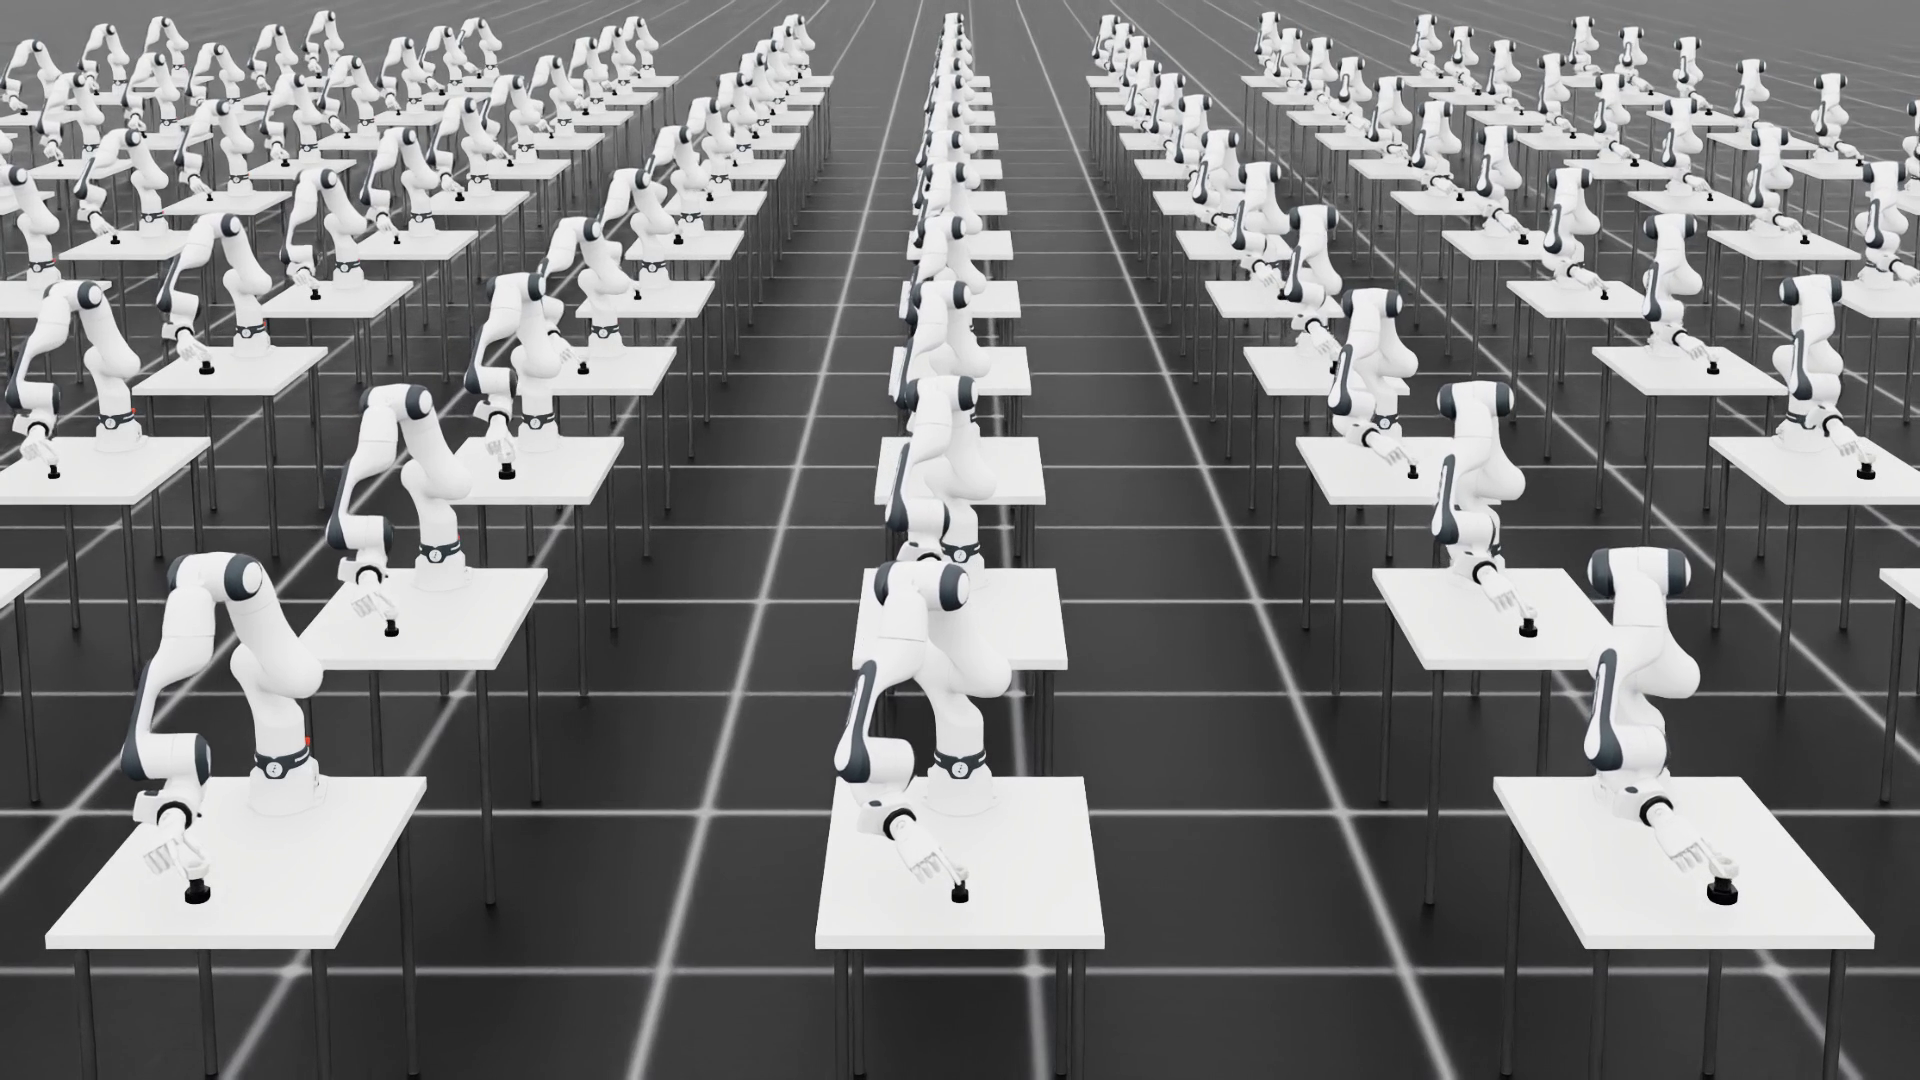
\includegraphics[width=\textwidth]{figures/policy_visuals/teacher/threading_v2_teacher_120_envs.png}
        \caption{Parallel teacher-training workcells.}
    \end{subfigure}\hfill
    \begin{subfigure}[b]{0.49\textwidth}
        \centering
        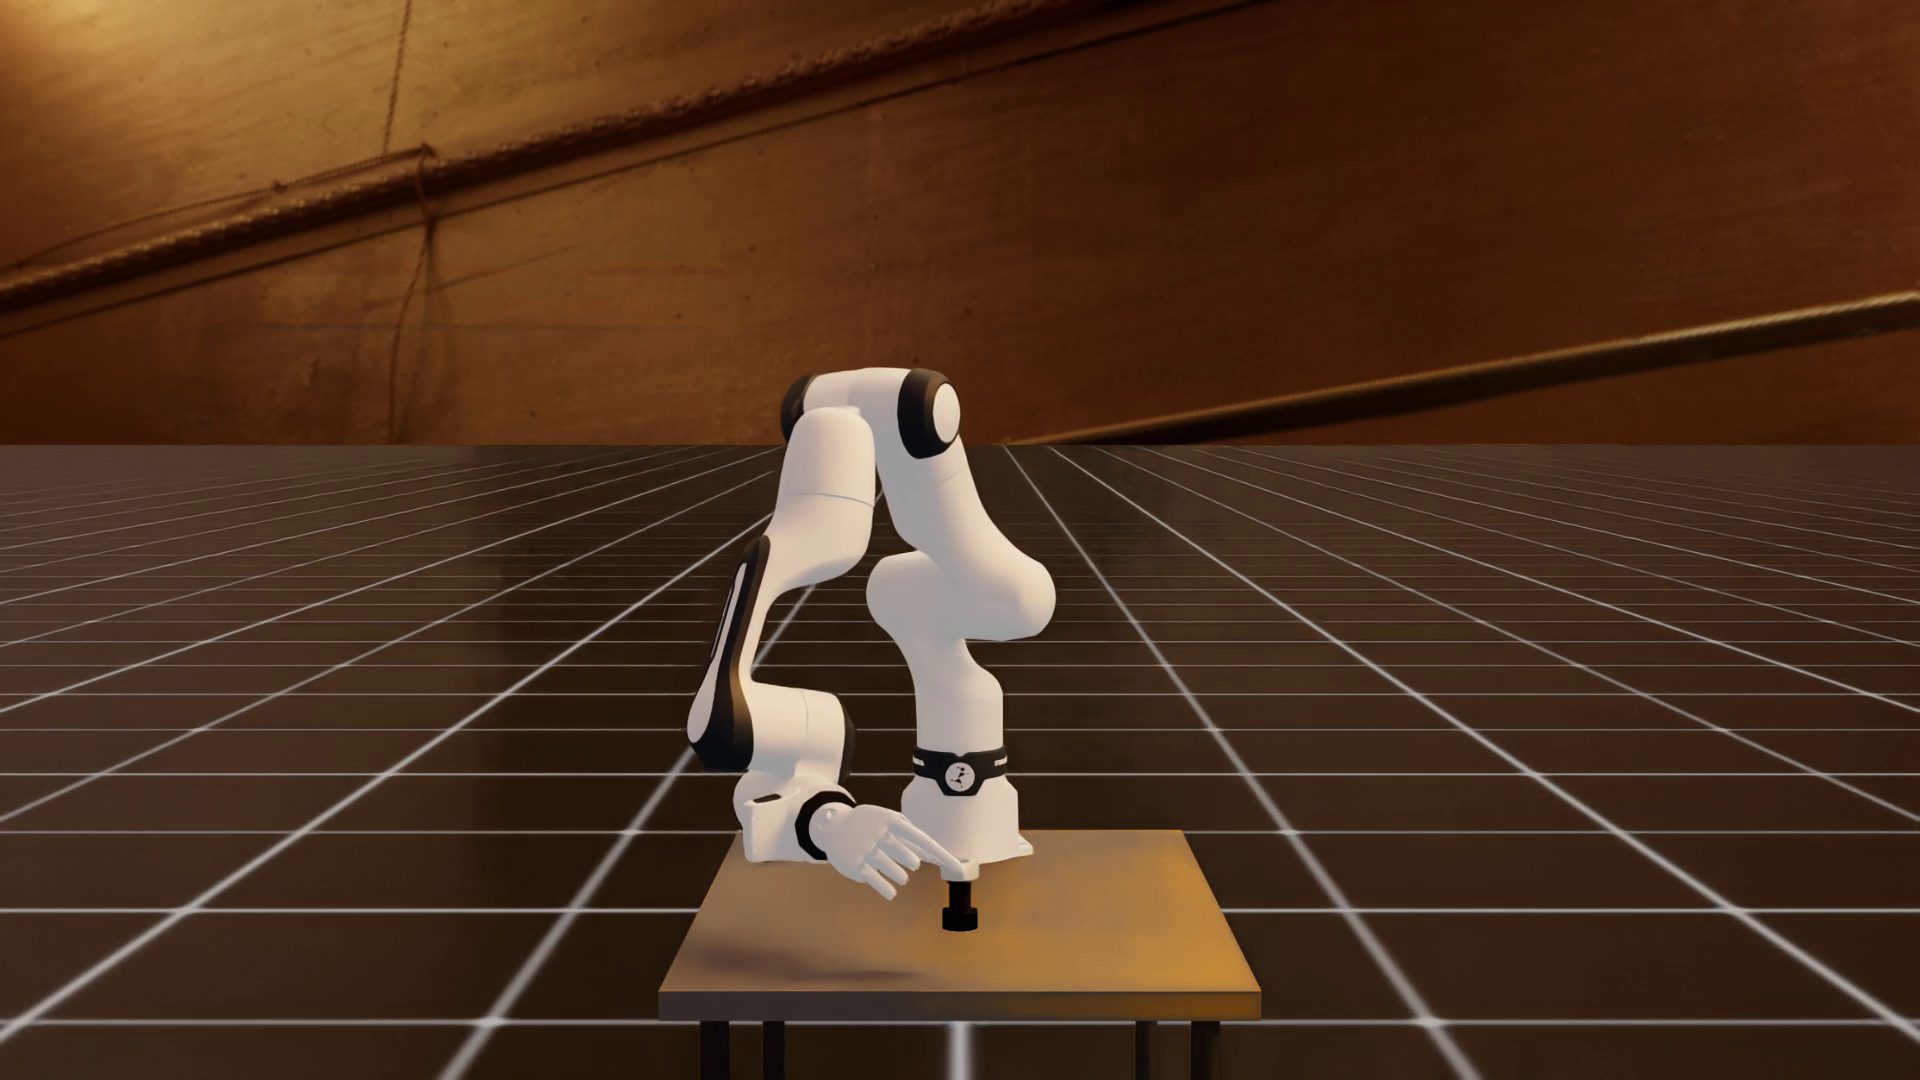
\includegraphics[width=0.49\textwidth]{figures/policy_visuals/teacher/randomization_dark.png}\hfill
        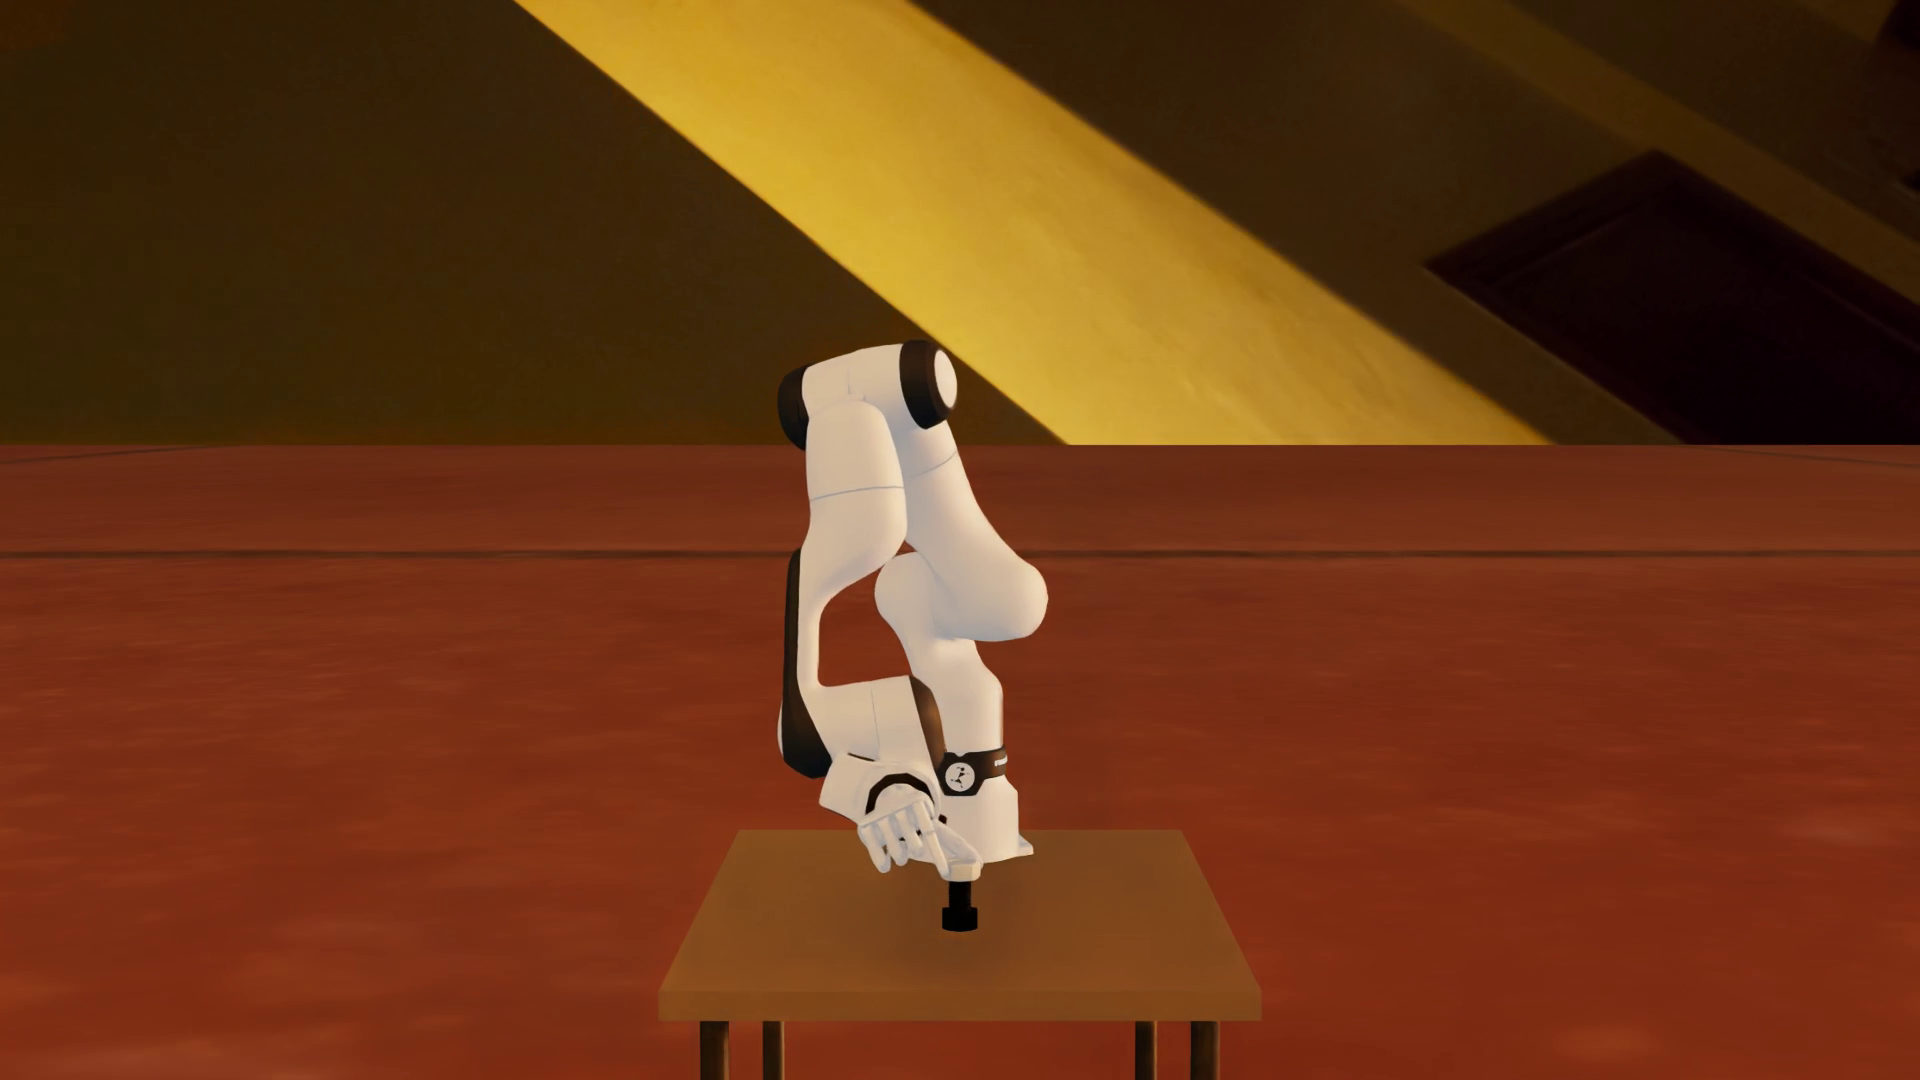
\includegraphics[width=0.49\textwidth]{figures/policy_visuals/teacher/randomization_warm.png}\\[1mm]
        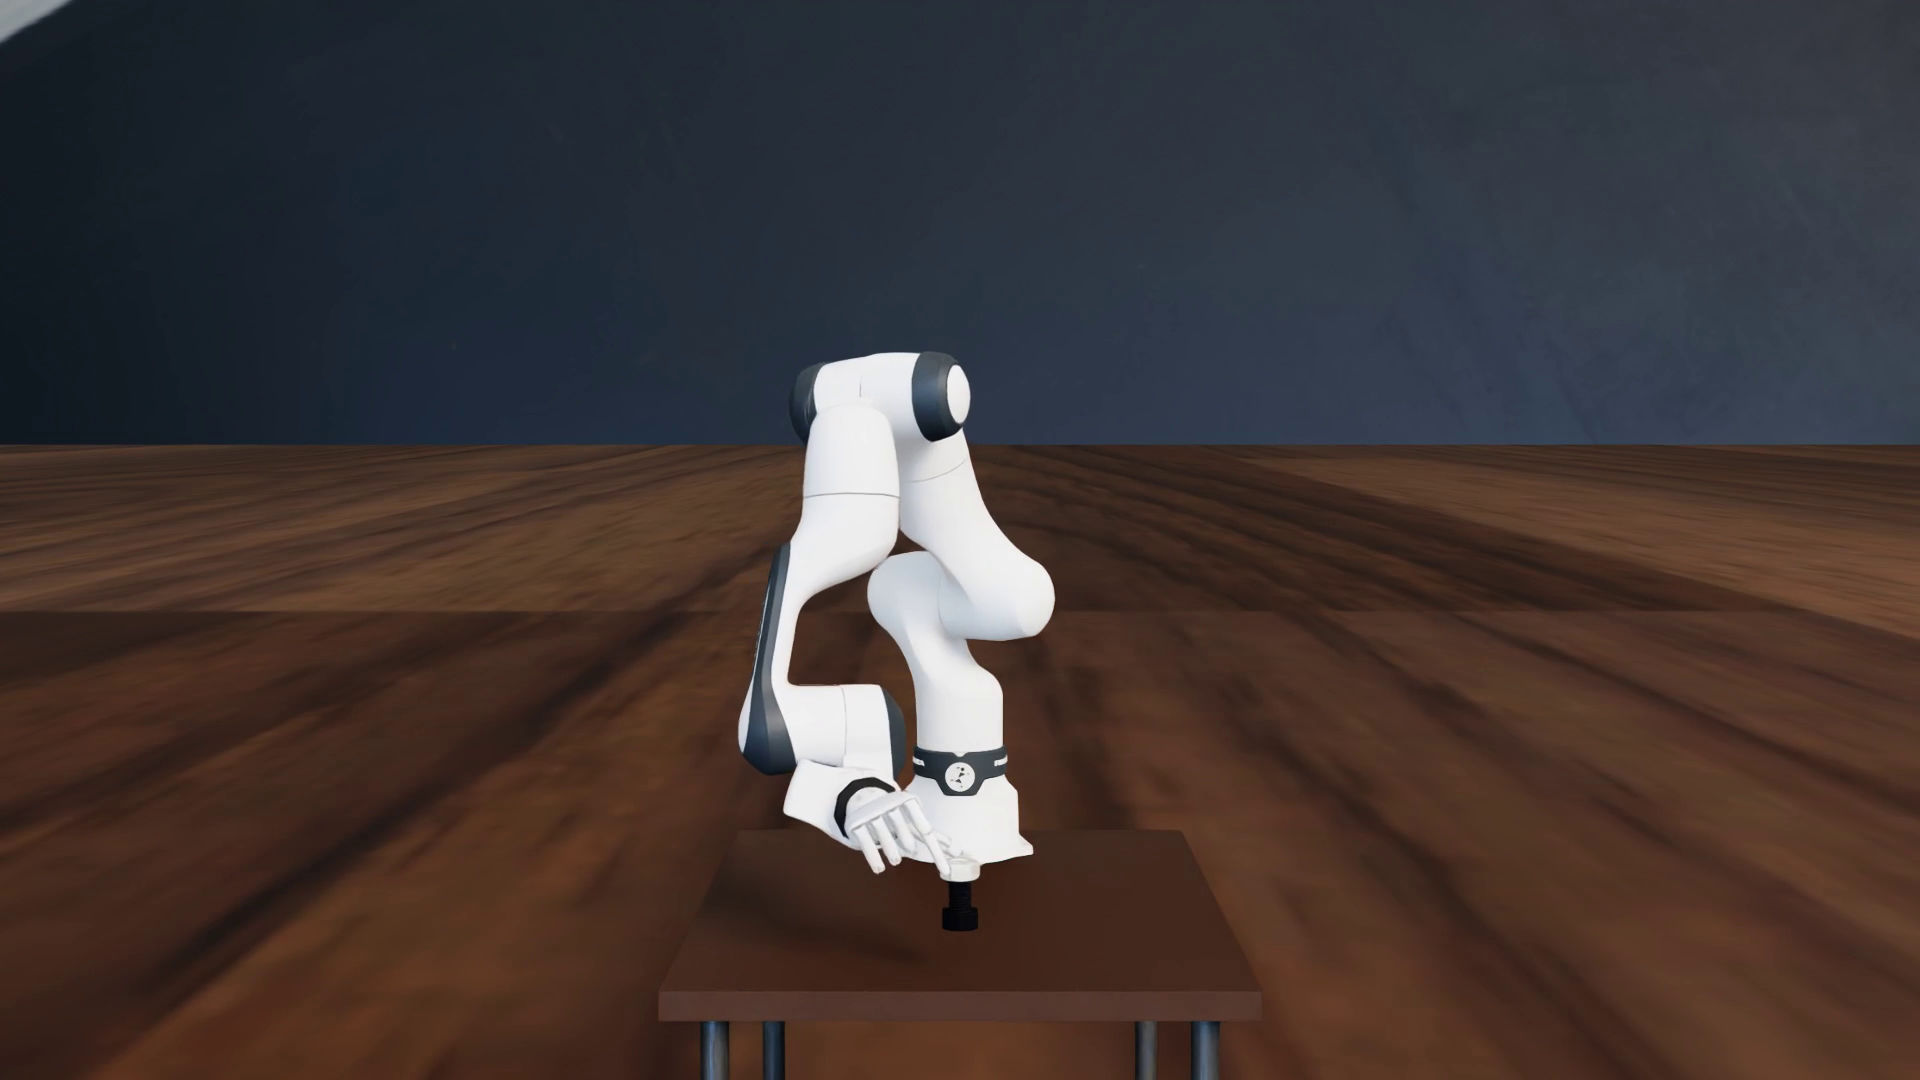
\includegraphics[width=0.49\textwidth]{figures/policy_visuals/teacher/threading_v2_lighting_texture_randomization.png}\hfill
        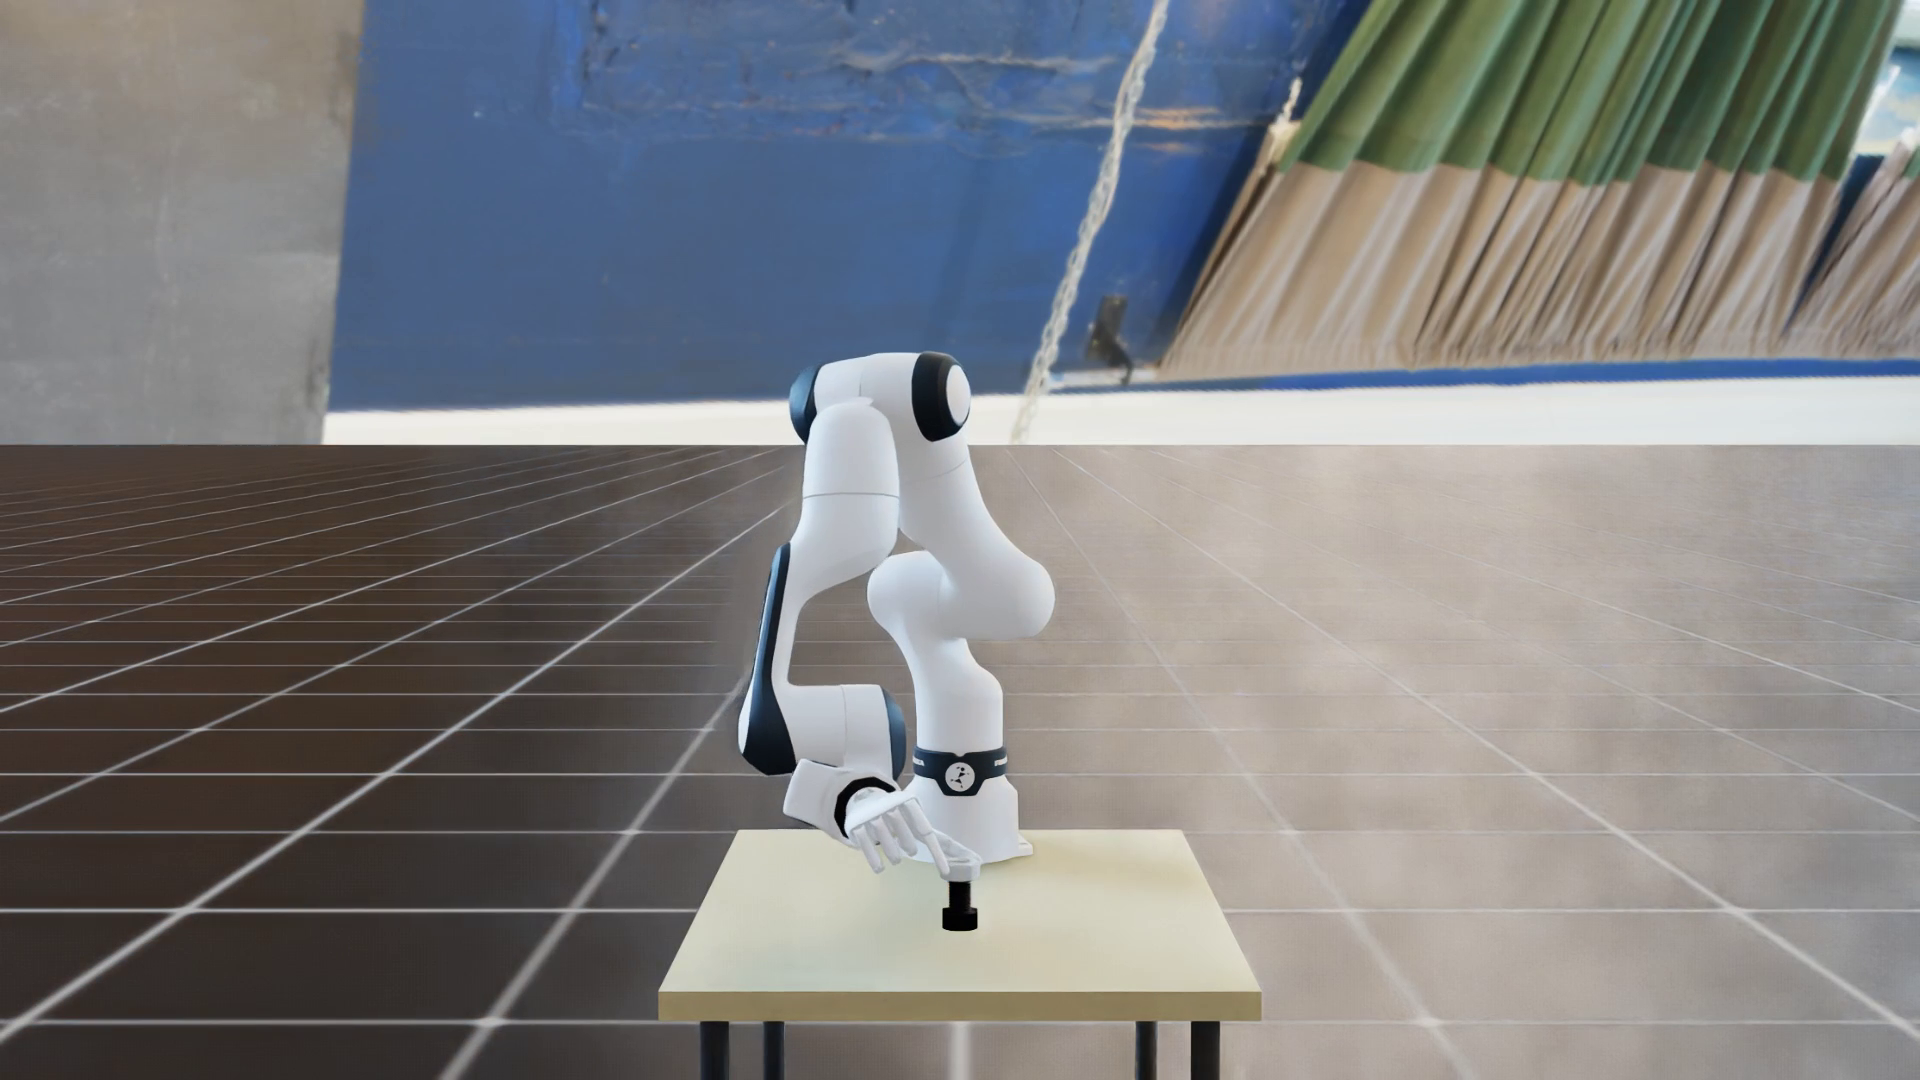
\includegraphics[width=0.49\textwidth]{figures/policy_visuals/teacher/randomization_blue.png}
        \caption{Lighting and texture randomization.}
    \end{subfigure}\\[2mm]
    \begin{subfigure}[b]{\textwidth}
        \centering
        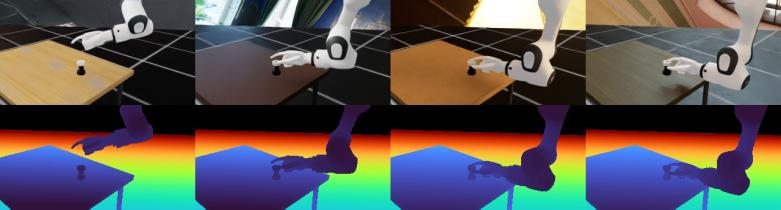
\includegraphics[width=0.8\textwidth]{figures/photos/sim_rgbd_strip.png}
        \caption{Student RGB (top) and depth (bottom) observations in simulation during approach, grasp, rotation, and release.}
    \end{subfigure}
    \caption{Simulation scenes. Teacher policies are trained in hundreds of parallel workcells rendered without visual randomization. Demonstrations for the student are rendered with randomized dome lighting, tabletop texture, and image background, and the student sees aligned RGB and metric depth of the resulting scene.}%
    \label{fig:sim-scenes}%
\end{figure}%

\section{Teacher Training}\label{sec:sim-teacher}

\label{sec:sim-experts}
Every demonstration comes from the hybrid teacher, so the teacher has to turn the nut reliably and hand over cleanly to the scripted release and return. The teacher result is also the experimental test of difficulty~(b) of Section~\ref{sec:problem-setup}: whether a learned policy acquires the pinch grasp and keeps it under the turning load through the commanded hand and arm degrees of freedom. With the simplified thread model and the three-stage reward of Section~\ref{sec:teacher}, the threading expert learns the single $60\degree$ turn from the engaged nut. On an earlier humanoid-arm platform, the recipe with the $\pm30\degree$ initial-yaw curriculum reached a population success rate of 83.6\,\% at the end of training, with a peak of 90.0\,\%. On the final platform, the retained M24 teacher, trained for 200 epochs with the curriculum and the axial-height randomization, completed ten consecutive cycles in all 32 hybrid-teacher candidate environments without a single transition failure. This is the property that matters for demonstration generation. The single-turn success rate of this teacher at the final curriculum level is \tbd.
% TODO(results): report final-epoch single-turn success and curriculum level of the retained FR3 M24 threading teacher (TensorBoard of the run promoted on 2026-09-10) and of the M24/M30/M36 multi-size teacher.
Table~\ref{tab:teacher-results} summarizes the teacher results. It shows that the teacher on the final platform meets the requirement of the student dataset, error-free transitions over ten cycles, while its single-turn success rates are still pending.

\begin{table}[htb]%
    \centering%
    \caption{Teacher training results. Success is the population success rate at the end of training. The hybrid-teacher column counts candidate environments that completed the required cycles with zero transition failures. The earlier platform is the humanoid arm on which the project started. The final platform is described in Section~\ref{sec:real-setup}.}%
    \label{tab:teacher-results}%
    \resizebox{\textwidth}{!}{%
\begin{tabular}{llccc}
        \toprule
        Teacher & Platform & Success & Peak success & Hybrid rollout \\
        \midrule
        Threading, $\pm30\degree$ yaw curriculum & earlier humanoid arm & 83.6\,\% & 90.0\,\% & -- \\
        Threading, M24, yaw and depth randomization & final & \tbd & \tbd & 32/32 ten-cycle \\
        Threading, M24/M30/M36 one-hot & final & \tbd & \tbd & \tbd \\
        \bottomrule
    \end{tabular}}
\end{table}%

All reported teachers use the Factory controller gains of Section~\ref{sec:action-contract}, and the physical controller is tuned toward these gains (Chapter~\ref{ch:real}).

\section{Student Ablations in Simulation}\label{sec:sim-student}

The main ablation study answers RQ1 and RQ2 of Section~\ref{sec:research-questions}. Five students are trained on the simulated dataset of Section~\ref{sec:dataset} and evaluated under matched budgets, and each ablation replaces one part of the full method: the training data in (a), the encoder in (b), and the generative action head in (c) and (d), where (c) also replaces the Transformer backbone. Ablation (a) addresses RQ1: it tests whether one student trained on multi-cycle data outperforms a single-cycle policy that is invoked repeatedly. Ablations (b) to (d) address RQ2: (b) replaces the point-cloud encoder with an image-space encoder, and (c) and (d) replace the flow-matching head with deterministic regression on a recurrent and on a Transformer backbone. RQ3 is evaluated on hardware in Chapter~\ref{ch:real}.

\begin{enumerate}
  \item[(a)] \emph{Single-cycle student.} The student is trained on demonstrations of one cycle and is invoked ten times in a trial. Its temporal context is reset after every cycle.
  \item[(b)] \emph{ResNet visual encoder.} The point-cloud encoder is replaced by the one-branch image-space encoder of Section~\ref{sec:student}, an ImageNet-pretrained ResNet-18 stage-2 trunk on RGB, log depth, and a validity mask, with an embedding of the calibrated camera-frame XYZ added on the token grid, that produces the same 64-D feature. Policy, objective, data, and budget are unchanged.
  \item[(c)] \emph{Point-cloud encoder with \ac{LSTM} regression.} The flow-matching Transformer is replaced by the DextrAH-RGB-style recurrent backbone of Section~\ref{sec:baselines}, a layer-normalized 512-unit \ac{LSTM} followed by a 512--512--256 ELU \acs{MLP}, trained by deterministic action regression on the same data.
  \item[(d)] \emph{Point-cloud encoder with Transformer regression.} The deterministic ACT-style Transformer of Section~\ref{sec:baselines} predicts the eight-step chunk from eight learned action queries.
  \item[(e)] \emph{Full method.} One flow-matching student with the point-cloud encoder is trained on the complete multi-cycle simulated demonstrations.
\end{enumerate}

Table~\ref{tab:ablation-sim} reports the results on the M24 hexagonal nut. The full method (e) completes all ten cycles in every trial, with a cyclic tracking error of $-1.77\pm1.02\degree$ and a ten-cycle error of $-17.7\pm3.23\degree$. The student thus lags the $60\degree$ target by less than two degrees per cycle, and the lag accumulates over the trial without its spread drifting. Each ablation removes one property on which this result may depend. The single-cycle student (a) never sees the axial advance of the nut: in a single-cycle demonstration the nut is always grasped at its reset height, whereas over ten cycles it advances down the bolt by one sixth of a pitch per cycle, and the multi-cycle student has to read this height from the point cloud (RQ1). The ResNet student (b) keeps everything but the representation. The regression students (c) and (d) keep the data and, for (d), also the backbone, the chunk length, and the temporal ensembling, so that their difference to (e) isolates the generative objective (RQ2). Their results on the simulated dataset are \tbd.
% TODO(results): retrain ablations (a)-(d) on the simulated-only ten-cycle M24 dataset and evaluate ten trials each. The previous runs (a 5.5+-0.8, b 2.3+-0.9 / +20.17+-7.80, c 0.0, d 1.4+-0.8 / +124.21+-18.50) included the real-world replay data and cannot be reused.

\begin{table}[htb]%
    \centering%
    \caption{Simulation ablations on the M24 hexagonal nut over ten trials. Each defined entry reports mean $\pm$ standard deviation. Completed cycles are averaged across trials, cyclic-error statistics use completed cycles only, and the ten-cycle error compares the accumulated rotation with the $600\degree$ target. It is reported as ``--'' when no trial completes all ten cycles. Errors are signed in degrees: negative denotes lag and positive overshoot.}%
    \label{tab:ablation-sim}%
    \small
    \begin{tabular}{lccc}
        \toprule
        Ablation & Completed cycles $\uparrow$ & Cyclic error $\rightarrow0$ & Ten-cycle error $\rightarrow0$ \\
        \midrule
        (a) single-cycle student & \tbd & \tbd & \tbd \\
        (b) ResNet encoder & \tbd & \tbd & \tbd \\
        (c) \ac{LSTM} regression & \tbd & \tbd & \tbd \\
        (d) Transformer regression & \tbd & \tbd & \tbd \\
        (e) full method & $10.0\pm0.0$ & $-1.77\pm1.02$ & $-17.7\pm3.23$ \\
        \bottomrule
    \end{tabular}
\end{table}%

For the encoder part of RQ2, a representation probe complements the closed-loop ablation (b). One shared pose decoder is trained on the frozen 64-D feature of each encoder to predict the nut position and orientation. A re-grasp needs exactly the orientation of the nut faces relative to the fingers, so the probe tests whether a representation carries the quantity on which the closed loop depends. The probe errors of the point-cloud and the ResNet features are \tbd.
% TODO(results): rerun the pose probe on the encoders of the simulated-only students (e) and (b). The previous probe (point cloud 8 mm / 15.16 deg, ResNet 8.6 mm / 31.20 deg) used encoders trained with the real-world replay data.

\section{Design Ablations of the Student}\label{sec:sim-design}

The main ablations compare the final student with alternatives at the level of whole components. The design of the student itself was fixed earlier by a sequence of controlled ablations, which this section reports because they explain why each component is present. The design ablations use six-cycle sequential-threading data. Except where a subsection varies them, all runs use the privileged 6-D nut-pose observation or the \acs{RGBD} observation as stated, 20 impulse-augmented demonstrations, 300 epochs, the Cartesian contract, $H=8$, and the student-owned cyclic evaluation with a six-cycle requirement at a fixed seed. Except for the ten-cycle \ac{DP3} student, these ablations were run on the earlier humanoid-arm platform. The threading results are matched single rollouts, not success rates.

\subsection{Progress and Phase Conditioning}\label{sec:sim-conditioning}

The global progress scalar lets the student finish all cycles, and the process-phase encoding keeps it synchronized with the physical cycle. On six-cycle sequential-threading demonstrations with policy-only impulses, a state-conditioned flow student completed four of the six cycles. With impulses in every phase segment and the global trajectory progress $p_t$ added to the condition, the student completed all six required cycles in 735 control ticks with zero transition failures. Its release times, however, drifted increasingly behind the teacher, by $+8.6$\,s at the sixth release, and the fifth cycle took twice as long as the others. Adding the three-way process-phase encoding reduced the completion time to 609 ticks and equalized the cycle durations to 6.7 to 7.1\,s. It also reduced the release-time errors against the teacher to within $\pm0.5$\,s, the controlled-joint \acs{RMSE} against the nominal trajectory from $11.5\degree$ to $4.7\degree$, the \acs{TCP} position \acs{RMSE} from 75\,mm to 28\,mm, and the final cumulative nut-turn error from $-60\degree$ to $-8\degree$. The offline teacher fit of the phase-conditioned checkpoint was marginally worse than that of the progress-only checkpoint (first-action \acs{RMSE} 0.0046 against 0.0044), so a better fit does not explain the closed-loop improvement. The phase encoding acts instead as a synchronization signal that keeps the student's internal clock aligned with physical events when the cycle duration deviates from nominal. All later students use both conditions. Table~\ref{tab:conditioning} collects the numbers.

\begin{table}[htb]%
    \centering%
    \caption{Conditioning ablation on six-cycle sequential threading (privileged 6-D observation, matched single rollouts at one seed). \acs{RMSE} values are against the nominal teacher trajectory in absolute time. The final turn error is the cumulative nut-rotation error after the last cycle.}%
    \label{tab:conditioning}%
    \resizebox{\textwidth}{!}{%
\begin{tabular}{lcccc}
        \toprule
        Condition & Cycles & Ticks & Joint \acs{RMSE} & Final turn error \\
        \midrule
        state only, policy-only impulses & 4/6 & 776 & $14.9\degree$ & -- \\
        state + progress $p_t$, all-phase impulses & 6/6 & 735 & $11.5\degree$ & $-60.3\degree$ \\
        state + progress + phase $\vec{e}^{m}_t$ & 6/6 & 609 & $4.7\degree$ & $-8.2\degree$ \\
        \bottomrule
    \end{tabular}}
\end{table}%

\subsection{Vision Encoder and Pretraining}\label{sec:sim-vision}

The visual students match the privileged student, and the retained \ac{DP3} encoder owes its accuracy to pretraining on rendered nut sweeps. The first \acs{RGBD} student used the two-branch cross-attention encoder with an auxiliary nut-position head and completed all six cycles in 617 ticks, matching the privileged student. A recollection with explicit success markers and retraining reproduced the result in 627 ticks. The retained \ac{DP3} encoder is pretrained on rendered sweeps of a free-moving nut from the calibrated camera and reaches a held-out position error of 5.9\,mm and a hexagon-symmetry-aware rotation error of $46\degree$. On the earlier platform, fine-tuning a sweep-pretrained encoder on hybrid-teacher images with phase-balanced sampling reduced these errors to 1.9\,mm and $3.8\degree$ on held-out teacher episodes, and to 2.8\,mm and $6.6\degree$ on images from a student rollout. The retained student does not use this fine-tuning stage. The ten-cycle \ac{DP3} student of Table~\ref{tab:ablation-sim} was initialized from this sweep-pretrained encoder with all encoder parameters trainable. It completed all ten cycles in 1072 ticks with a maximum turn of $60.3\degree$ and a mean absolute retained-turn error of $3.1\degree$. Its release times lag those of its source demonstration by 2.7\,s on average and by 7.4\,s at the tenth cycle, a timing drift that does not affect the completion of the cycles. Table~\ref{tab:encoders} prepares a closed-loop comparison of the \ac{DP3}, Adapt3R-style, ResNet, two-branch, and depth-only encoders under identical data and budget, which extends ablation (b). Its results are \tbd.
% TODO(results): train offline_flow_matching_adapt3r_agent.yaml and the one-channel ResNet encoder on the ten-cycle M24 dataset with the same recipe as the DP3 student; evaluate ten trials each.

\begin{table}[htb]%
    \centering%
    \caption{Vision-encoder ablation of the flow student on the ten-cycle M24 task (ten trials). The \acs{DP3} row is the full method. The remaining rows are placeholders.}%
    \label{tab:encoders}%
    \resizebox{\textwidth}{!}{%
\begin{tabular}{lccc}
        \toprule
        Encoder & Completed cycles $\uparrow$ & Cyclic error $\rightarrow0$ & Ten-cycle error $\rightarrow0$ \\
        \midrule
        point cloud, DP3-style (RGB + XYZ) & $10.0\pm0.0$ & $-1.77\pm1.02$ & $-17.7\pm3.23$ \\
        ResNet-18 early fusion (b) & \tbd & \tbd & \tbd \\
        Adapt3R-style (frozen ResNet + 3D attention) & \tbd & \tbd & \tbd \\
        Two-branch cross-attention \acs{RGBD} & \tbd & \tbd & \tbd \\
        Depth-only CNN & \tbd & \tbd & \tbd \\
        \bottomrule
    \end{tabular}}
\end{table}%

\subsection{Privileged Observations, Horizon, Integration Steps, and Inputs}\label{sec:sim-sweeps}

The privileged observation modes serve as upper bounds and as diagnostics. With the nut position (3-D) or pose (6-D) appended to the proprioception instead of the visual feature, the same flow student is trained and evaluated without rendering. On six-cycle sequential threading, the privileged 6-D student and the \acs{RGBD} student both completed six cycles at matched settings, which shows that the visual feature carries the information the task needs. The remaining sweeps over the action horizon $H$, the number of Euler steps $N$, the temporal-ensemble decay, the hand-velocity input, and the terminal-hold padding are implemented as command-line options of the offline trainer and evaluator but have not been run as controlled studies. Table~\ref{tab:sweeps} gives the skeleton. Once filled, it will show how sensitive the reference student is to each of these choices and what inference latency each number of Euler steps costs.
% TODO(results): run action-horizon sweep (H in {1, 4, 8, 16}), ODE-step sweep (N in {1, 4, 8, 16, 32}), temporal-ensemble decay in {0, 0.5, 0.8}, and --hand-velocity-observation omitted on the ten-cycle M24 dataset; ten trials each; also record inference latency per N.

\begin{table}[htb]%
    \centering%
    \caption{Student hyperparameter sweeps on the ten-cycle M24 task (ten trials). All cells are placeholders except the reference row.}%
    \label{tab:sweeps}%
    \resizebox{\textwidth}{!}{%
\begin{tabular}{llccc}
        \toprule
        Sweep & Value & Completed cycles $\uparrow$ & Cyclic error $\rightarrow0$ & Latency \\
        \midrule
        reference & $H=8$, $N=16$, decay 0.5 & $10.0\pm0.0$ & $-1.77\pm1.02$ & \tbd \\
        horizon $H$ & 1 / 4 / 16 & \tbd & \tbd & \tbd \\
        Euler steps $N$ & 1 / 4 / 8 / 32 & \tbd & \tbd & \tbd \\
        ensemble decay & 0 / 0.8 & \tbd & \tbd & -- \\
        hand velocities omitted & 26-D proprioception & \tbd & \tbd & -- \\
        privileged 3-D / 6-D nut pose & no vision & \tbd & \tbd & -- \\
        \bottomrule
    \end{tabular}}
\end{table}%

\subsection{Nut-Size Conditioning, Domain Randomization, and Force Observations}\label{sec:sim-robustness}

Three further ablations are implemented but not yet qualified in simulation. First, the multi-size teacher conditions on a one-hot code of M24, M30, and M36 with round-robin assignment and per-size meshes, keypoints, and pitches. A multi-size student would be trained on hexagonal nuts of all three sizes without an explicit size input and would have to infer the size from the point cloud. Its per-size simulation results are \tbd. The hardware results across sizes are reported in Chapter~\ref{ch:real}. Second, physical domain randomization of mass, friction, controller gains, and reset pose is enabled during teacher training and disabled during demonstration collection and evaluation. Its effect on the student when enabled at evaluation time is \tbd. Third, hardware-equivalent force observations are implemented as observation channels for both teacher and student: the thumb and index flexion forces projected onto the pad normals, and the seven arm joint reaction torques normalized by the joint torque limits of the arm. They are not yet part of any trained contract, and their effect is \tbd. Table~\ref{tab:robustness} lists the skeleton, which will show how far the student tolerates size variation, physical perturbation, and additional force input.
% TODO(results): (i) per-size ten-trial evaluation of the multi-size student in simulation; (ii) evaluation with --enable-domain-randomization; (iii) teacher and student retrained with the fingertip-force and joint-torque channels enabled in the actor/student vectors.

\begin{table}[htb]%
    \centering%
    \caption{Robustness ablations in simulation (ten trials of ten cycles). All cells are placeholders.}%
    \label{tab:robustness}%
    \resizebox{\textwidth}{!}{%
\begin{tabular}{llccc}
        \toprule
        Ablation & Condition & Completed cycles $\uparrow$ & Cyclic error $\rightarrow0$ & Ten-cycle error $\rightarrow0$ \\
        \midrule
        nut size & M24 / M30 / M36 & \tbd & \tbd & \tbd \\
        physical \acs{DR} at evaluation & off / on & \tbd & \tbd & \tbd \\
        force observations & none / fingertip / fingertip + torque & \tbd & \tbd & \tbd \\
        axial-height curriculum & 20\,mm / \tbd & \tbd & \tbd & \tbd \\
        \bottomrule
    \end{tabular}}
\end{table}%

\section{Offline versus Online Distillation}\label{sec:sim-online}

The offline flow students with progress and phase conditioning complete every required cycle, whereas the online \ac{DAgger} students complete at most two. The comparison uses online \ac{DAgger} with the recurrent \ac{LSTM} student on cyclic threading from privileged 6-D observations under the Cartesian contract, with the hybrid teacher as the label source and a ten-cycle cap per episode. In these runs, the intervention schedule determined which part of the cycle the online student learned. The decayed run was trained without physical domain randomization, unlike the two fixed schedules. Under full teacher control ($\beta=1$) it learns the threading turn. Under full student control ($\beta=0$) with teacher labels it learns the turn and the complete release-and-return transition. With an intervention probability that decays linearly from full teacher to full student control, it learns both and completes two uninterrupted student-only turn-release-return cycles. The offline flow student completes all six cycles of the conditioning study with privileged observations and all ten cycles from \acs{RGBD}. Table~\ref{tab:online} summarizes the comparison.
% TODO(results): the online flow-matching student (Section 3.5.5) is implemented; train online_dagger_flow_matching on cyclic_threading with nut_pose_6d (beta=1, H=8), evaluate ten trials, and add it to Table 4.5 if it qualifies.

\begin{table}[htb]%
    \centering%
    \caption{Offline and online distillation on cyclic threading (privileged 6-D observation unless stated, Cartesian contract). Cycles are student-only completed cycles of the best retained checkpoint in one evaluation rollout. The offline rows are matched single rollouts from Section~\ref{sec:sim-design}.}%
    \label{tab:online}%
    \resizebox{\textwidth}{!}{%
\begin{tabular}{llcc}
        \toprule
        Student & Intervention & Completed cycles & Learned behavior \\
        \midrule
        online \ac{DAgger} \ac{LSTM} & $\beta=1$ & 0 & threading turn \\
        online \ac{DAgger} \ac{LSTM} & $\beta=0$ & 1 & turn and transition \\
        online \ac{DAgger} \ac{LSTM} & $\beta$ decayed $1\rightarrow0$ & 2 & turn and transition, two cycles \\
        online \ac{DAgger} \ac{LSTM} & SafeDAgger 0.10/0.075 & 0 & approach \\
        offline flow, state + progress + phase & -- & 6/6 & complete cycle, Table~\ref{tab:conditioning} \\
        offline flow, \acs{RGBD} & -- & 10/10 & complete cycle, Table~\ref{tab:ablation-sim} \\
        \bottomrule
    \end{tabular}}
\end{table}%

The evaluation ladder of Section~\ref{sec:ladder} shows that the offline fit does not explain this difference. Table~\ref{tab:ladder-results} places several offline students on its first rung next to their closed-loop outcome. Every listed checkpoint reproduces its training labels with first-action \acs{RMSE} below 0.04 in the student's action units and correlation above 0.99. The offline fit is therefore a necessary diagnostic and not a predictor of task success. The closed-loop outcome follows the contract, the conditioning, and the data. The retained student combines the three properties that the closed loop rewards: the Cartesian contract, the progress and phase conditions, and demonstrations that contain the teacher's recoveries from disturbances in every phase. Together with chunked prediction and temporal ensembling, these properties plausibly let it recover from its own deviations under its own observations, which is the regime in which the online recurrent students fall behind.

\begin{table}[htb]%
    \centering%
    \caption{Offline teacher-fit against closed-loop outcome for offline flow students (\acs{EMA} weights, sixteen Euler steps, one training episode). \acs{RMSE} values are in the bounded 9-D action units of the student.}%
    \label{tab:ladder-results}%
    \resizebox{\textwidth}{!}{%
    \begin{tabular}{llcccl}
        \toprule
        Student & Data & First-action \acs{RMSE} & Chunk \acs{RMSE} & Correlation & Closed loop \\
        \midrule
        Cartesian, 6-D nut pose, state only & 6-cycle threading, policy impulses & 0.0050 & 0.0110 & 0.9996 & 4/6 cycles \\
        Cartesian, 6-D nut pose, + progress & 6-cycle, all-phase impulses & 0.0044 & 0.0122 & 0.9997 & 6/6 cycles \\
        Cartesian, 6-D nut pose, + progress + phase & 6-cycle, all-phase impulses & 0.0046 & 0.0129 & 0.9997 & 6/6 cycles \\
        Cartesian, \acs{RGBD} two-branch, + aux.\ head & 6-cycle, all-phase impulses & 0.0044 & 0.0055 & 0.9997 & 6/6 cycles \\
        Cartesian, \ac{DP3} from sweep pretraining & 10-cycle, all-phase impulses & 0.019 & 0.019 & 0.994 & 10/10 cycles \\
        \bottomrule
    \end{tabular}}
\end{table}%

\section{Ablation Inventory}\label{sec:sim-inventory}

Table~\ref{tab:inventory} lists every ablation that the code base exposes as a configuration, with the table or section that reports its result or the placeholder that awaits one. The inventory follows the three ablation axes of the student, namely the vision encoder, the action head, and the observation and action contract, and adds the teacher, data, and evaluation options around them. It shows which design choices are backed by a result and which remain open.

\begin{table}[htb]%
    \centering%
    \caption{Inventory of ablations supported by the code base. ``Result'' names the table or section with a result. \tbd{} marks an ablation whose result is pending.}%
    \label{tab:inventory}%
    \resizebox{\textwidth}{!}{%
\begin{tabular}{llll}
        \toprule
        Axis & Ablation & Options & Result \\
        \midrule
        student & behavior cloning (joint history \acs{MLP}) & diagnostic only & Section~\ref{sec:baselines} \\
        student & online \ac{DAgger} \ac{LSTM} & $\beta$ fixed, decayed, SafeDAgger & Table~\ref{tab:online} \\
        student & offline flow matching & Transformer; \acs{MLP} backbone \tbd & Table~\ref{tab:ablation-sim} \\
        student & online \ac{DAgger} flow matching & $\beta=1$, $H=8$ & \tbd \\
        student & regression heads & \ac{LSTM} (c), Transformer (d) & \tbd \\
        vision & encoder & \ac{DP3}, Adapt3R, ResNet (b), two-branch, depth-only & Tables~\ref{tab:ablation-sim}, \ref{tab:encoders} \\
        vision & \ac{DP3} initialization & scratch, sweep pretraining & Section~\ref{sec:sim-vision} \\
        vision & depth corruption in pretraining & none, Gaussian, realistic & \tbd \\
        observation & privileged vs visual & nut XYZ, nut 6-D, \acs{RGBD} & Section~\ref{sec:sim-sweeps} \\
        observation & hand velocities & included, omitted & \tbd \\
        observation & force channels & fingertip force, joint torque & \tbd \\
        observation & phase encoding & none, process phase & Table~\ref{tab:conditioning} \\
        observation & progress scalar & none, global progress & Table~\ref{tab:conditioning} \\
        action & horizon $H$, steps $N$, ensemble decay & sweep & \tbd \\
        teacher & intervention schedule & see student & Table~\ref{tab:online} \\
        teacher & nut-size conditioning & M24, M30, M36 & Chapter~\ref{ch:real}, \tbd \\
        data & disturbance augmentation & none, policy-only, all phases & Table~\ref{tab:conditioning} \\
        data & visual domain randomization & on, off & \tbd \\
        data & physical domain randomization & on, off & \tbd \\
        evaluation & ladder & offline fit, closed loop & Table~\ref{tab:ladder-results} \\
        \bottomrule
    \end{tabular}}
\end{table}%

\section{Summary}\label{sec:sim-summary}

In simulation, the hybrid teacher produces error-free ten-cycle demonstrations, and the full method trained on them completes all ten cycles of the M24 task in every trial with a cyclic error of $-1.77\pm1.02\degree$. The design ablations support the Cartesian contract and the progress and phase conditions, together with demonstrations that contain recoveries from disturbances in every phase, and they show that the offline fit alone does not predict it. Whether the multi-cycle data (RQ1) and the point-cloud encoder and flow-matching head (RQ2) are each necessary will be settled by the reruns of ablations (a) to (d) on the simulated dataset. Simulation cannot show whether the student bridges the gap in contact and perception that the simplified thread model and the rendered images leave open. Chapter~\ref{ch:real} therefore deploys the same student, trained on simulated data only, on the physical system to answer RQ3.
%
% !TeX spellcheck = en_US
\chapter{Experiments on Real Hardware}\label{ch:real}%

Chapter~\ref{ch:sim} showed that the distilled student sustains consecutive threading cycles in simulation. This chapter asks whether that behavior survives the gap between the simplified simulation and the physical workcell, which is RQ3 of Section~\ref{sec:research-questions}: can a student trained on simulated demonstrations only transfer zero-shot to the physical system? No real-world data enters training, and nothing is trained on the robot. Section~\ref{sec:real-setup} introduces the physical system, including the robot, the camera and its calibration, the controller, the measurement of the nut angle, and the test objects. Section~\ref{sec:real-transfer} describes the zero-shot transfer protocol. Section~\ref{sec:real-results} reports the closed-loop results on the M24 training nut, Section~\ref{sec:real-geometry} on unseen nut geometries, and Section~\ref{sec:real-stress} under long-horizon stress.

\section{Hardware Setup}\label{sec:real-setup}

The physical workcell, shown in Figure~\ref{fig:real-setup}, is the platform of Section~\ref{sec:platform}: the \ac{FR3} arm with the Inspire RH56DFX right hand and the three commanded pinch degrees of freedom described there. The bolt stands on a 5\,cm pedestal on a 60\,cm by 80\,cm bench, and the robot base is mounted at tabletop height, 46.5\,cm from the near table edge, so that the reach envelope lies above the work surface.

The simulated system is a model of this workcell. The transform of the adapter flange was measured and reproduced in the simulated asset. The hand asset was regenerated from the official robot URDF that ships with this hand, which carries the measured pivot geometry of the fingers. Joint limits and link inertias are those of the URDF, and linear mimic ratios approximate the linkage that couples the finger joints of the physical hand. The \ac{FR3} is the arm that replaced the earlier humanoid-arm platform of Section~\ref{sec:platform}.

A fixed Intel RealSense D415 on a stand provides the \acs{RGBD} observation at $640\times480$. As in simulation, the stream is center-cropped and downscaled to the $320\times180$ policy input (Figure~\ref{fig:real-rgbd}). The pose of the camera relative to the robot base was deduced from twelve different poses of a calibrated AprilTag observed by the camera, with a translation fit \acs{RMSE} of 27\,mm and a rotation fit \acs{RMSE} of $3.5\degree$ over the calibration poses. The calibrated optical pose and the intrinsics are the ones used to render the simulated camera and to back-project the point cloud, so the student sees the same geometry in both domains.
% TODO(unsure): the calibration artifact is labeled "measured", not "deployment validated"; confirm whether a refined calibration was used for the reported hardware trials. The 27 mm / 3.5 deg RMSE here and in Chapter 6 come from the 2026-09-10 calibration. The current forgeUltra camera_info.yaml holds the 2026-10-29 calibration: 12 samples collected, 11 used, 9.7 mm / 0.98 deg.

Robot commands use the same Cartesian impedance law as in simulation, so the student's bounded action reaches the arm through the shared action path of Section~\ref{sec:action-contract}. The deployment controller is derived from the libfranka Cartesian-impedance example controller and modified to follow \eqref{eq:osc}, including the axis-angle orientation error and the dynamically consistent nullspace term. The modifications are described below. Gravity is compensated by libfranka, which matches the simulation, where gravity is disabled for the arm. The controller runs at the 1\,kHz rate of the Franka control interface, while the student commands targets at 15\,Hz. The hand is position-controlled through its serial interface. The task-space gains equal those of the simulation, 565\,N/m and 28\,N\,m/rad with critical damping, and the nullspace stiffness is 10. The mapping of the student's bounded action to the controller target is \tbd.
% TODO(results): document the physical controller gains, the target low-pass settings, and the hand command rate used in the hardware trials (libfranka tooling on the franka-chi branch).

\paragraph{Controller families.}
The unmodified libfranka example differs from the Factory controller of \eqref{eq:osc} in three places. It uses a damped kinematic nullspace projector built from a pseudoinverse of the Jacobian transpose with regularization 0.2, it feeds the rotational spring the vector part of the error quaternion instead of the rotation vector, and it adds the robot's Coriolis term. Near the threading posture, the damped projector lets the posture spring push 12.5\,N on the tool at a 1\,rad wrist excursion, comparable to the 11.3\,N that the policy commands for a 20\,mm position step, whereas the exact projector reduces this to 0.4\,N.
% TODO(unsure): forgeUltra has no source for the 12.5 / 11.3 / 0.4 N figures; confirm their origin.
 The quaternion vector halves the effective rotational stiffness from 28 to 14\,N\,m/rad. The deployment controller therefore replaces all three: it uses the dynamically consistent projector with the arm mass matrix from the robot model, with the hand configured as end-effector load, the rotation-vector error, and no Coriolis term, because the simulated arm is not compensated either. Both backends are implemented in the simulation with selectable gains, so a teacher can be trained under either. The reported teachers use the Factory controller, and the physical controller reproduces it rather than the other way around. The student's commands therefore meet the stiffness under which the teacher acquired its contact behavior.

\paragraph{Trajectory export.}
For open-loop validation of the action path, every simulated demonstration can be exported as a command-only deployment artifact. The simulator recording is authoritative for the geometric joint path. Some scripted phases, however, change the joint position kinematically while writing zero articulation velocity, so the export does not use recorded velocities. It fits one twice continuously differentiable quintic curve through the recorded positions and derives position, velocity, and acceleration from it, with deployment limits on joint positions and velocities applied explicitly. On the \acs{FR3} the Cartesian targets are executed directly through the libfranka-style controller, which keeps open-loop playback and student execution on the same path.

\paragraph{Angle measurement and test objects.}
The metrics of Section~\ref{sec:metrics} require the nut angle. It is read from an angular scale printed on a sheet under the bolt pedestal (Figure~\ref{fig:real-phases}), and the unwrapped angle is recorded at the end of every goal-reaching phase. The test-object family, shown on the right of Figure~\ref{fig:real-setup}, consists of M24, M30, and M36 nuts in four profiles each, hexagonal, octagonal, rectangular, and round, with matching bolts and holders. Teacher and student training use the hexagonal profiles only. The other three profiles are held out for the generalization study of Section~\ref{sec:real-geometry}.

\begin{figure}[htb]%
    \centering%
    \begin{subfigure}[b]{0.49\textwidth}
        \centering
        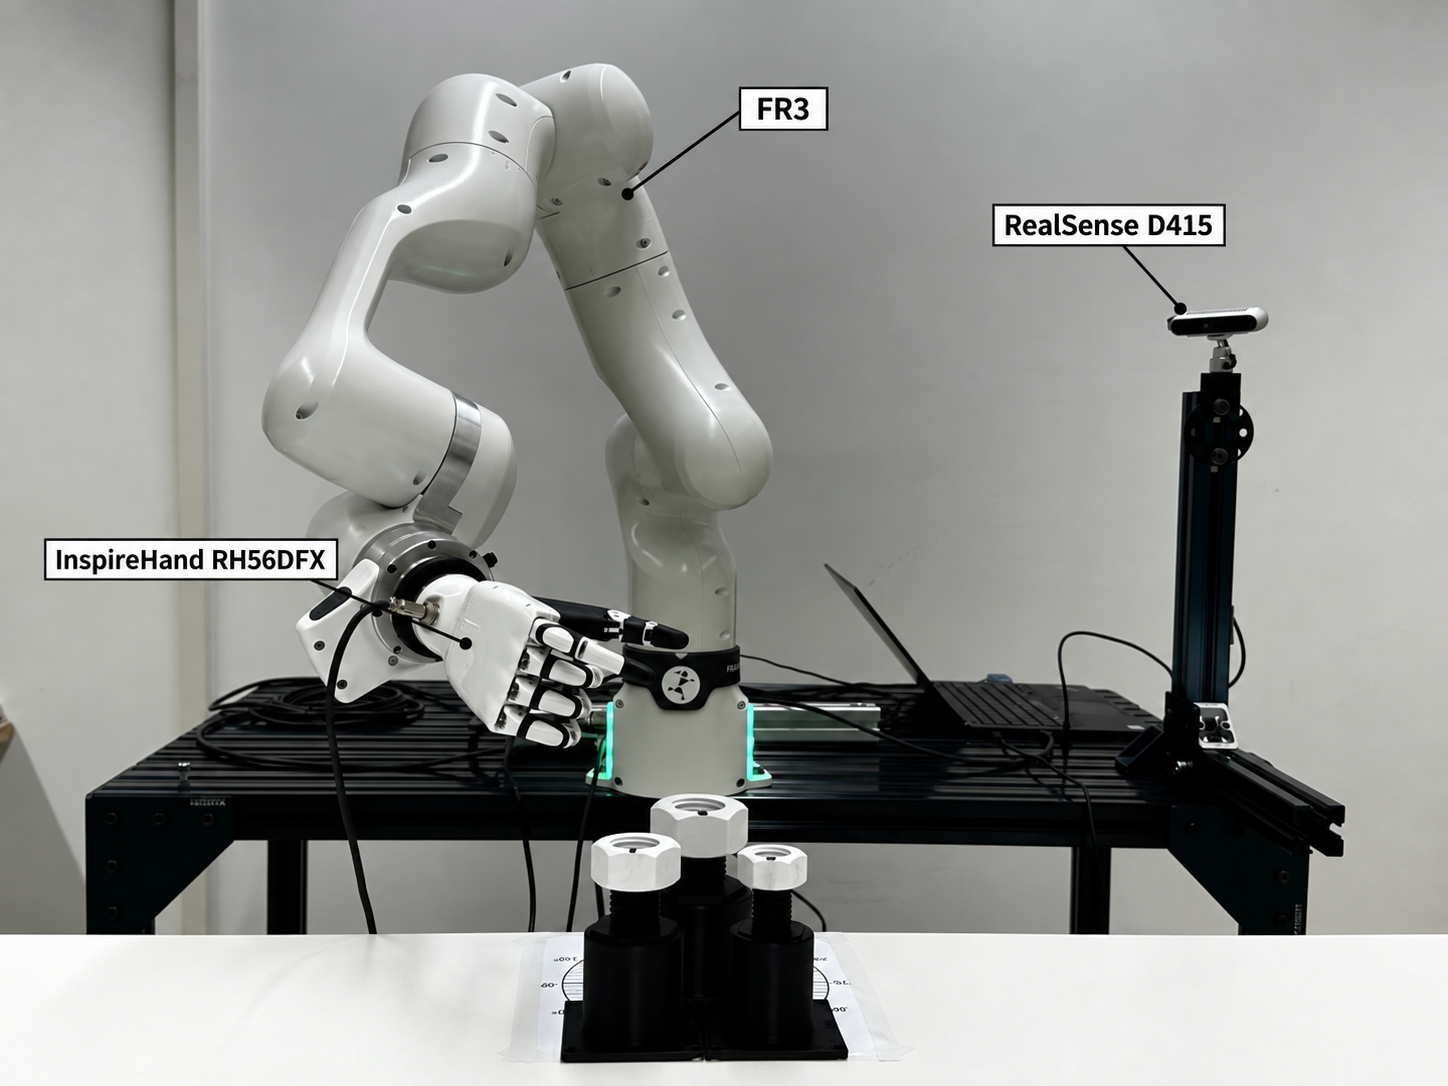
\includegraphics[width=\textwidth]{figures/hardware_setup_annotated.png}
        \caption{Physical workcell.}
    \end{subfigure}\hfill
    \begin{subfigure}[b]{0.49\textwidth}
        \centering
        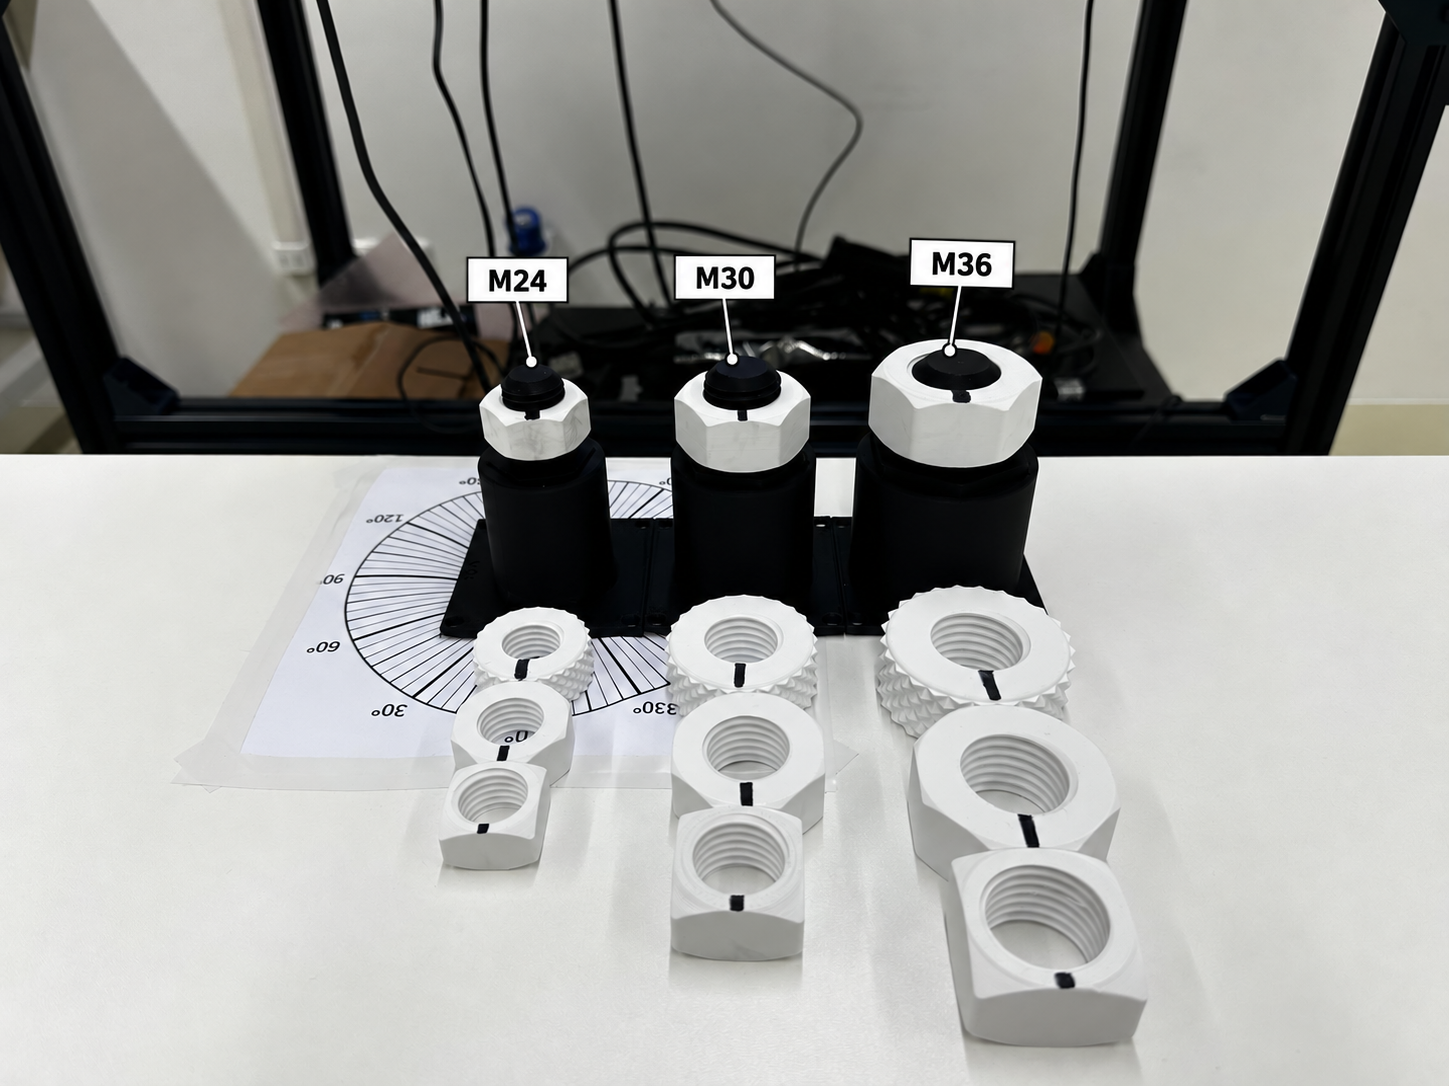
\includegraphics[width=\textwidth]{figures/NutBoltHolderFamilyOnly2_annotated.png}
        \caption{Test-object family.}
    \end{subfigure}
    \caption{Hardware setup. Left: the \acs{FR3} arm with the Inspire RH56DFX hand, the bolts on their holders in front of the robot, and the fixed RealSense D415 on its stand. Right: M24, M30, and M36 bolts with the hexagonal, octagonal, rectangular, and round nuts of each size. Only the hexagonal nuts are used for training.}%
    \label{fig:real-setup}%
\end{figure}%

\begin{figure}[htb]%
    \centering%
    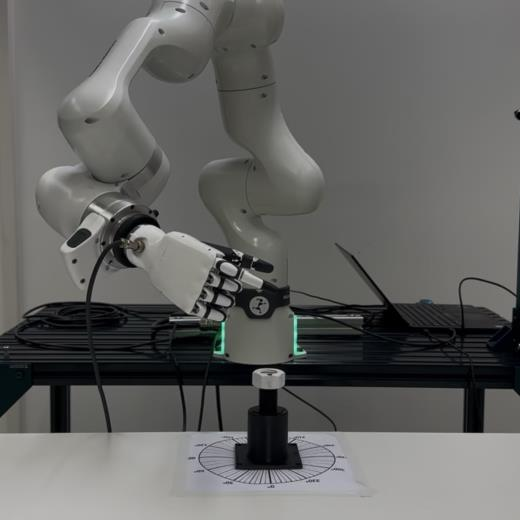
\includegraphics[width=0.19\textwidth]{figures/photos/real_approach.png}\hfill
    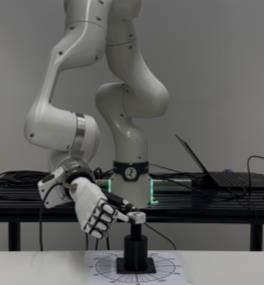
\includegraphics[width=0.19\textwidth]{figures/photos/real_grasp.png}\hfill
    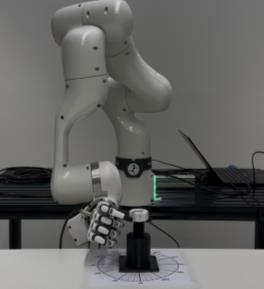
\includegraphics[width=0.19\textwidth]{figures/photos/real_rotate.png}\hfill
    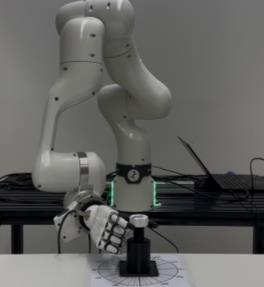
\includegraphics[width=0.19\textwidth]{figures/photos/real_goal.png}\hfill
    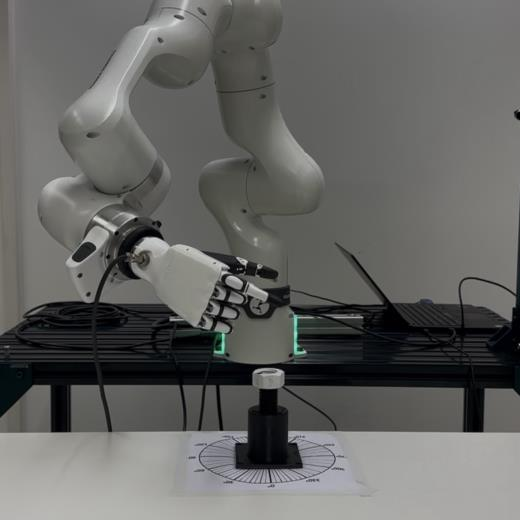
\includegraphics[width=0.19\textwidth]{figures/photos/real_release.png}\\[1mm]
    \hspace*{0.2\textwidth}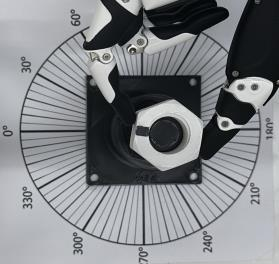
\includegraphics[width=0.19\textwidth]{figures/photos/dial_grasp.png}\hfill
    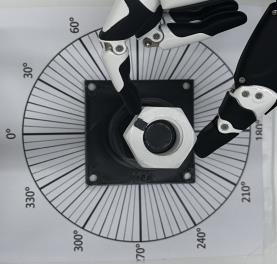
\includegraphics[width=0.19\textwidth]{figures/photos/dial_rotate.png}\hfill
    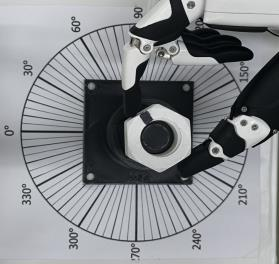
\includegraphics[width=0.19\textwidth]{figures/photos/dial_goal.png}\hspace*{0.2\textwidth}
    \caption{One threading cycle on the physical robot. Top, from left to right: approach, grasp, rotation, goal reaching, and release with return to the reset pose. Bottom: top-down views of the angular scale under the bolt during grasp, rotation, and goal reaching. The scale is read at the end of every goal-reaching phase to compute the cyclic and ten-cycle tracking errors.}%
    \label{fig:real-phases}%
\end{figure}%
% TODO(figure): these photos were taken during the earlier hardware trials; retake them with the zero-shot student, or confirm that they are suitable as an illustration of the phases.

\begin{figure}[htb]%
    \centering%
    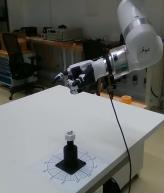
\includegraphics[height=0.3\textwidth]{figures/photos/real_rgb.png}\hspace{6mm}%
    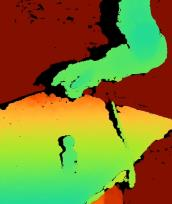
\includegraphics[height=0.3\textwidth]{figures/photos/real_depth.png}
    \caption{Student observation on the physical system: the RGB image (left) and the metric depth image (right) of the RealSense D415 after center-cropping and downscaling to $320\times180$. The depth image is back-projected through the calibrated intrinsics into the point cloud that the student encodes.}%
    \label{fig:real-rgbd}%
\end{figure}%

\section{Zero-Shot Transfer Protocol}\label{sec:real-transfer}

The protocol tests RQ3 directly: the student is trained on simulated data only and deployed unchanged. The student of the full method is trained for 300 epochs on the simulated dataset $\Dset=\Dsim$ of Section~\ref{sec:dataset} with eight-step chunks. It is deployed on the physical robot with a prediction horizon of eight and sixteen \ac{ODE} integration steps. No real-world images, trajectories, or corrections enter its training, and it is not fine-tuned on the robot. The transfer therefore rests entirely on four properties of the pipeline. The calibrated camera of Section~\ref{sec:real-setup} is the one that rendered the demonstrations. The point-cloud crop box removes the physical background before encoding. The demonstrations were rendered under lighting, texture, and background randomization. The Cartesian targets are executed by the impedance controller described above. The student receives the progress scalar from the elapsed trial time and the process phase from the physical events of the cycle, as in simulation (Section~\ref{sec:student}).
% TODO(results): document the deployment settings of the zero-shot trials (checkpoint, depth preprocessing on the physical D415, phase-signal source on hardware).

\section{Results on the Training Nut}\label{sec:real-results}

Table~\ref{tab:ablation-real} is the hardware counterpart of the simulation ablation on the M24 hexagonal nut. It answers RQ3 on the training nut, and it checks whether the comparisons of RQ1 and RQ2 carry over to hardware. Three of the five students are taken to hardware: the full method (e), the single-cycle student (a), and the ResNet student (b). The single-cycle student tests whether the advantage of multi-cycle distillation persists on the physical system, and the ResNet student tests whether the image-space representation transfers as well as the point cloud. The two regression heads (c) and (d) are evaluated in simulation only. The hardware results are \tbd.
% TODO(results): run ten zero-shot M24 trials each for (e), (a), and (b) once the simulated-only students are retrained and the randomization ranges are fitted to the physical sensor (Section 3.4.4). For reference: the earlier zero-shot hardware run of the simulated-only student completed 2.1+-1.4 cycles with a cyclic error of -10.05+-4.08 deg; the earlier full-method hardware numbers came from a student trained with real-world replay data and cannot be reused.

\begin{table}[htb]%
    \centering%
    \caption{Real-world zero-shot ablations on the M24 hexagonal nut over ten trials, with the same conventions as Table~\ref{tab:ablation-sim}. Ablations (c) and (d) are evaluated in simulation only.}%
    \label{tab:ablation-real}%
    \small
    \begin{tabular}{lccc}
        \toprule
        Ablation & Completed cycles $\uparrow$ & Cyclic error $\rightarrow0$ & Ten-cycle error $\rightarrow0$ \\
        \midrule
        (a) single-cycle student & \tbd & \tbd & \tbd \\
        (b) ResNet encoder & \tbd & \tbd & \tbd \\
        (e) full method & \tbd & \tbd & \tbd \\
        \bottomrule
    \end{tabular}
\end{table}%

\section{Generalization across Nut Sizes and Geometries}\label{sec:real-geometry}

The training nut alone does not show how far the zero-shot transfer reaches, so the full method is also evaluated on all twelve test objects. Table~\ref{tab:geometry} reports ten trials per object: the M24, M30, and M36 hexagonal nuts, whose profile the demonstrations show, and the octagonal, rectangular, and round profiles of each size, which it has never seen. The study tests two kinds of generalization. Across sizes, the student must infer the nut size from the point cloud, since it receives no explicit size input. Across profiles, the question is whether the learned pinch-and-re-grasp strategy, which the demonstrations show only on hexagons, transfers to a different face topology. The results are \tbd.
% TODO(unsure): Section sec:dataset describes an M24-only dataset; confirm whether the hardware student is trained on M24 only or on the multi-size data of Section sec:sim-robustness, and state the training sizes here.
% TODO(results): run the twelve-object zero-shot evaluation (ten trials per nut). The earlier geometry results came from a student trained with real-world replay data and cannot be reused.
% TODO(results): the earlier values (student trained with real-world replay data) were removed; fill in the zero-shot results.

\begin{table}[htb]%
    \centering%
    \caption{Real-world zero-shot transfer across nut sizes and profiles over ten trials per nut. Values are mean $\pm$ standard deviation. The octagonal, rectangular, and round profiles and the M30 and M36 sizes are absent from the demonstrations.}%
    \label{tab:geometry}%
    \small
    \begin{tabular}{llccc}
        \toprule
        Size & Profile & Completed cycles $\uparrow$ & Cyclic error $\rightarrow0$ & Ten-cycle error $\rightarrow0$ \\
        \midrule
        \multirow{4}{*}{M24} & hexagonal & \tbd & \tbd & \tbd \\
         & octagonal & \tbd & \tbd & \tbd \\
         & rectangular & \tbd & \tbd & \tbd \\
         & round & \tbd & \tbd & \tbd \\
        \midrule
        \multirow{4}{*}{M30} & hexagonal & \tbd & \tbd & \tbd \\
         & octagonal & \tbd & \tbd & \tbd \\
         & rectangular & \tbd & \tbd & \tbd \\
         & round & \tbd & \tbd & \tbd \\
        \midrule
        \multirow{4}{*}{M36} & hexagonal & \tbd & \tbd & \tbd \\
         & octagonal & \tbd & \tbd & \tbd \\
         & rectangular & \tbd & \tbd & \tbd \\
         & round & \tbd & \tbd & \tbd \\
        \bottomrule
    \end{tabular}
\end{table}%

\section{Long-Horizon Stress}\label{sec:real-stress}

Beyond the ten-cycle protocol, the student is run on hardware for as many cycles as it sustains, to measure how far its horizon extends beyond the ten cycles of the demonstrations. Every revolution advances the nut by one pitch down the bolt. After enough cycles, the nut therefore leaves the axial range that the ten-cycle demonstrations cover. The stress trials thus measure how far the learned behavior reaches along the bolt. The cycle counts per nut are \tbd.
% TODO(results): run the long-horizon stress trials with the zero-shot student and tabulate the sustained cycle count per nut size and profile.

Together, the three studies provide the hardware evidence for RQ3: transfer on the training nut, generalization across sizes and profiles, and the reach of the behavior beyond the demonstrated horizon. Chapter~\ref{ch:discussion} interprets this evidence alongside the simulation results of Chapter~\ref{ch:sim}.
%
% !TeX spellcheck = en_US
\chapter{Discussion}\label{ch:discussion}%

This chapter interprets the results of Chapters~\ref{ch:sim} and~\ref{ch:real}. Section~\ref{sec:disc-ablations} answers the three research questions of Section~\ref{sec:research-questions} as far as the available results allow. Section~\ref{sec:disc-contracts} draws the lesson of the action and observation contracts. Section~\ref{sec:disc-assembly} returns to the assembly motivation and asks how far the demonstrated skill is from industrial threading. Section~\ref{sec:disc-limitations} states the limitations of the work.

\section{Interpretation per Research Question}\label{sec:disc-ablations}

All three research questions presuppose a teacher that produces complete multi-cycle demonstrations, so the teacher result comes first. \ac{PPO} learns the threading turn once the thread is constrained kinematically and the learned task is one turn from an engaged nut. The kinematic constraint makes the learning problem well posed: it ties axial progress to rotation, so the progress reward can only be earned by turning. The teacher also answers difficulty~(b) of Section~\ref{sec:difficulty-dexterity}: with the hand restricted to three commanded pinch degrees of freedom, it acquires the pinch grasp and keeps it under the turning load, and losing the grasp after it has latched ends the episode, which makes grasp retention a hard constraint (Section~\ref{sec:teacher}). Trained under initial-yaw, axial-height, and controller randomization, the retained teacher, chained into the hybrid teacher, produces the successful ten-cycle demonstrations of the student dataset (Section~\ref{sec:dataset}). The \ac{RL} teacher solves one turn, and the hybrid rollout extended it to ten consecutive cycles. The turn also needs no force sensing: the actor of the retained teacher observes no force channel. Hardware-equivalent force observations are implemented for teacher and student and remain to be evaluated.
% TODO(unsure): appendix tab:teacher-obs lists thumb/index flexion force as actor inputs (39-D); confirm that the retained teacher actor has no force channel (see TODO in appendix.tex).

RQ1 asks whether one student distilled from multi-cycle demonstrations sustains consecutive cycles, and it tests the deployment side of difficulty~(c) of Section~\ref{sec:difficulty-horizon}. The full method completes all ten cycles in every simulated trial and lags the target by less than two degrees per cycle. The content of the data is the likely reason. In a single-cycle demonstration the nut is always grasped at its reset height, so a student trained on it never has to read the height from the point cloud. In a multi-cycle demonstration the nut descends by one sixth of a pitch per cycle, and the student learns to track it. The global progress scalar supports the multi-cycle student, but it does not supply the axial information. That information comes from the coverage of the axial state in the demonstrations. The single-cycle ablation (a) receives the same progress scalar and therefore isolates this effect. Its result is \tbd. RQ1 thus tests the principle that unifying the complete cyclic behavior in one dataset, rather than invoking a per-cycle policy repeatedly, yields a policy that sustains consecutive cycles.

RQ2 asks which student design makes the unification work. It has two parts, the visual representation and the action head, and each of the ablations (b) to (d) changes one of them. On the representation side, the student does not need to localize the nut to sub-millimeter accuracy. The engagement of the nut on the bolt and the compliance of the impedance controller absorb lateral error. What the student needs is the orientation of the nut faces for the re-grasp and the height of the nut for the approach. A representation that encodes position but not orientation would let the fingers close on the right spot with the wrong face alignment. The point-cloud encoder consumes the metric geometry of nut, bolt, and hand directly. It has about 60\,000 parameters and no pretrained image backbone. The pose probe of Section~\ref{sec:sim-student} tests whether the feature of each encoder carries the face orientation. The image-space encoder of ablation (b) also receives depth and per-pixel coordinates, so (b) tests whether the geometric structure of the representation, rather than the depth input alone, decides the closed-loop result. Random point sampling adds an augmentation that the image encoder does not receive. The closed-loop ablation (b) and the pose probe quantify the difference. Their results are \tbd.

On the head side, the chunked Transformer regression head (d) shares the backbone, the chunk length, and the temporal ensembling of the flow student, so the difference between (d) and (e) isolates the generative objective. Two mechanisms could favor the flow head. The first is multimodality of the labels. For near-identical observations, the dataset contains the teacher's nominal action in one demonstration and its recovery after an impulse in another. A squared-error head converges to their average, an action that neither demonstration contains, whereas the flow head samples one of them. The second is the structure of the prediction. The flow head predicts a velocity from a noisy chunk toward the data, a denoising problem that may be easier to fit than a direct regression from observation to chunk. Through the sixteen integration steps it refines all eight steps of the chunk jointly, with full attention among them. The recurrent regression head (c) additionally removes chunking. The results of (c) and (d) on the simulated dataset are \tbd.

RQ3 asks whether a student trained on simulated data only transfers zero-shot to the physical system, and it tests the transfer side of difficulty~(a) of Section~\ref{sec:difficulty-sim2real}. The transfer rests on four properties of the pipeline. The calibrated camera model is meant to make the simulated and real point clouds geometrically comparable. The crop box removes the background, which is where rendered and real images differ most. Lighting, texture, and background randomization, together with image-space color augmentation, are meant to cover the remaining appearance variation of the points that enter the encoder. The shared Cartesian action path executes the student's commands through a controller that reproduces the simulated control law, and the teacher was trained under randomized gains and noisy pose inputs. The same geometric property that RQ2 relies on matters here: inside the crop box the point geometry is identical in both domains up to depth noise and calibration error, whereas an image-space encoder faces the appearance gap of the full image. The per-point colors still carry the appearance gap of nut, bolt, and hand. The approach requires no real-world data collection and no training on the robot. The hardware results that test it are \tbd.
% TODO(results): compare the new zero-shot trials with the earlier sim-only hardware baseline once the trials of Chapter 5 are run.

\section{Action and Observation Contracts}\label{sec:disc-contracts}

The student imitates the teacher's bounded, bolt-relative Cartesian action. This keeps it in the teacher's own action space, expresses every target relative to the bolt tip, and executes the command through the unchanged controller, including the action smoothing that the teacher was trained with. A student should therefore imitate the action the teacher produced, in the units the teacher produced it, and let the controller do the conversion it was designed for.

The observation contract follows the same logic. The student receives the previous filtered action, which the teacher also observes, the positions and velocities of the ten controlled joints, which the teacher actor does not observe, and two low-dimensional conditions that the demonstration provides without privileged state. The global progress scalar assumes a nominally timed trial. For trials that run much longer than the demonstrations, the phase should be inferred from the observation history inside the policy rather than supplied as an external signal. Chapter~\ref{ch:conclusion} returns to this as future work.

\section{What This Means for Robotic Assembly}\label{sec:disc-assembly}

The motivation of this thesis was assembly with threaded joints (Section~\ref{sec:motivation}). Measured against an industrial fastening step, the demonstrated skill covers the run-down of an engaged nut and leaves four gaps.

The first gap is the start of the task. Every trial starts with the nut already engaged on the bolt (Section~\ref{sec:thread-model}). In assembly the nut arrives loose and has to be seated on the thread first, which is a separate skill with a narrow entry configuration. Engagement is therefore not covered by the demonstrated skill.

The second gap is the end of the task. A trial ends after ten turns of $60\degree$, which advance the nut by one and two thirds of a pitch, 5.0\,mm on the M24 nut. The nut is never seated against a part, and it is never tightened to a preload.
% TODO(cite): tightening to a specified torque or preload as the final step of threaded-joint assembly.
The simulated thread resists the turn only with a smoothed friction torque whose Coulomb term is $2\times10^{-3}$\,N\,m, which models a free-running nut. The actor observes no force, and the reward penalizes excess wrist force. A tightening phase would demand that the pinch transmit a much larger torque and that the policy sense when the joint is tight, which neither the thread model nor the observation contract supports.

The third gap is the grasp. The student executes one strategy, a thumb--index pinch with three commanded hand joints, learned on the face topology of a hexagon. People change the grasp as the resistance grows (Section~\ref{sec:difficulty-dexterity}), and a tightening phase would likely require such a change. The held-out octagonal, rectangular, and round profiles of Section~\ref{sec:real-geometry} test how far the single strategy carries. Their results are \tbd.

The fourth gap is cycle time. In the demonstrations, release and return take a nearly fixed time in every cycle, since their scripted waypoints are interpolated over 0.7\,s per segment and 1.0\,s for the final return. Because each cycle turns the nut by $60\degree$, a full revolution takes six cycles, which is far slower than the continuous rotation of a powered spindle.
% TODO(cite): typical run-down speed or cycle time of an industrial nutrunner, if a comparison is wanted.

These gaps do not erase what the result shows. In simulation, a learned policy controlled a dexterous hand through ten cycles of grasp, turn, release, and return, and it re-grasped the nut at the angle and height that the previous cycle left it. It perceives the nut from one fixed camera, and it is trained without any real data. The same hand also picks up a loose nut in simulation. Whether this versatility outweighs the speed of a dedicated tool depends on the application, and the remaining gaps define the work that separates the two (Chapter~\ref{ch:conclusion}).

\section{Limitations}\label{sec:disc-limitations}

Section~\ref{sec:disc-assembly} described the task-level gaps to industrial threading. This section states the limitations of the method and of the evidence. The demonstrated behavior is a pinch-grasp re-grasp strategy, and the student has no mechanism to discover a different grasp for a profile that requires one. The demonstrations start at the nominal nut height and cover only the 5.0\,mm of axial travel of ten cycles, and the global progress clock is defined over the nominal trial length. The teacher's thread model is a kinematic simplification. In simulation the nut therefore cannot jam or cross-thread, and the thread resists only through a small friction torque on the revolute joint. The randomization ranges that are meant to cover the resulting sim-to-real gap have not yet been fitted to measured statistics of the physical sensor. The camera calibration has a translation fit \acs{RMSE} of 27\,mm and a rotation fit \acs{RMSE} of $3.5\degree$ (Section~\ref{sec:real-setup}). It is measured but not deployment-validated, and the dependence of the student on calibration error has not been quantified. The evaluation uses ten trials per condition and reports means and standard deviations without confidence intervals. Chapter~\ref{ch:conclusion} summarizes what the thesis achieved and turns these gaps and limitations into future work.
% TODO(results): update RQ1 to RQ3, Section 6.4, and the limitations once the retrained ablations (a)-(d), the pose probe, and the zero-shot hardware trials are available.
%
% !TeX spellcheck = en_US
\chapter{Conclusion and Future Work}\label{ch:conclusion}%

This chapter summarizes what the thesis achieved, answers the research questions, and outlines the work that remains between the demonstrated skill and robotic assembly with threaded joints.

\section{Conclusion}\label{sec:conclusion}

Threaded joints can be released again and their threads are standardized~\cite{Budynas2020}, and fastening a nut is still largely left to people and specialized tools. This thesis asked how a dexterous robot can learn to thread a nut. Threading poses three difficulties at once. The skill has to be learned in simulation and transferred to hardware, although thread contact is hard to simulate. A dexterous hand has a large action space and many ways to solve the task. Threading is a long-horizon cyclic task in which errors compound across cycles and phase transitions.
% TODO(cite): nut fastening in industry is largely manual or done by specialized tools (reuse the citation of Section 1.1 once it exists).

The thesis answers these difficulties with one principle: decompose during data generation, unify at deployment. During data generation the cycle is decomposed into a turning skill and scripted transitions. A privileged asymmetric actor--critic learns the pinch-grasp turn in a simplified thread simulation in which axial progress follows from rotation. Scripted release and return chain the turns into a hybrid teacher that produces complete multi-cycle demonstrations with physically gated phase boundaries. At deployment the behavior is unified again. One visuomotor student, distilled from the demonstrations by conditional flow matching, executes the whole cycle from an \acs{RGBD} camera and proprioception. It was trained on simulated data only, and a calibrated camera model, a metric point cloud cropped to the workspace, visual domain randomization, and a shared Cartesian action path are designed to carry it to hardware.

The evidence in simulation is consistent with the principle. The single-cycle comparison that tests it (RQ1) is \tbd. Chained into the hybrid teacher, the \ac{RL} teacher completed ten consecutive cycles in all 32 candidate environments. The distilled student completes all ten cycles in every trial on the M24 hexagonal nut, with a mean cyclic tracking error of $-1.77\degree$ and a ten-cycle error of $-17.7\degree$. The single-seed design studies show why the action contract, the conditioning, and the disturbance augmentation of the student are present. The Cartesian action contract turns an equally good offline fit into closed-loop progress. The progress and phase conditions keep the student synchronized with the physical cycle. Demonstrations with recoveries in every phase plausibly let it correct its own deviations, which is where the online recurrent students fell behind.

The three research questions are answered as follows.
\begin{enumerate}
  \item[RQ1] One student distilled from complete multi-cycle demonstrations sustains all ten cycles in simulation, and its comparison with a single-cycle policy invoked repeatedly is \tbd.
  \item[RQ2] The flow-matching student with a point-cloud encoder sustains the cyclic task, and its comparison with deterministic \ac{LSTM} and Transformer regression and with an image-space encoder is \tbd.
  \item[RQ3] The student is trained on simulated data only and deployed without real data or training on the robot, and the result of its zero-shot transfer on the M24, M30, and M36 nuts and on held-out profiles is \tbd.
\end{enumerate}
% TODO(results): complete the RQ1 to RQ3 answers once the retrained ablations (a)-(d) and the zero-shot trials of Chapter 5 are available.

Returning to the motivation of Section~\ref{sec:motivation}: in simulation, a dexterous hand can now thread a nut over ten consecutive cycles with a learned policy, re-grasping it in every cycle from camera data at the angle and height that the previous cycle left it, and the policy is trained without real data. Whether it does so on the physical system is \tbd{} (RQ3). What it cannot yet do is start from a loose nut, tighten the joint, choose a different grasp when the resistance grows, or match the speed of a dedicated tool (Section~\ref{sec:disc-assembly}). These gaps define the future work.

\section{Future Work}\label{sec:future-work}

The first extension is autonomous engagement of a loose nut. It requires grasping the loose nut, transporting it to the bolt, and chaining these steps with threading. Seating the nut on the bolt is a separate skill with a narrow entry configuration. It will most likely require fingertip-force and tactile feedback, and the hardware-equivalent fingertip-force and joint-torque observation channels that are implemented for teacher and student are the starting point.

The second extension is tightening to a preload. A threading cycle that ends with the nut tight needs a thread model whose resistance rises when the nut seats, a grasp that transmits the resulting torque, and a policy that senses when the joint is tight. The same force channels are the natural inputs for such a policy.

The third extension is a longer horizon. The demonstrations start at the nominal nut height and cover only the 5.0\,mm of axial travel of ten cycles. A curriculum that widens this range toward the full usable thread length would extend the horizon of the teacher and of the student with it. The global progress clock should be replaced at the same time, because it binds the student to a nominal trial duration. Inferring the phase from the observation history inside the policy would remove that dependency.

The fourth extension concerns the transfer. The randomization ranges of the simulated camera should be fitted to measured statistics of the physical D415, including depth failures, exposure, motion blur, and camera and control latency. The depth-corruption model that the encoder pretraining already provides can then be applied to the student's training data as well.

The fifth extension concerns the grasp. Training on more than one face topology would extend the re-grasp strategy to profiles that a hexagon does not cover, and other grasp topologies than the thumb--index pinch would let the hand adapt its grasp to the resistance of the thread.

The last extension completes the distillation study. The online flow-matching student is implemented and remains to be evaluated. Collecting multi-step teacher recovery fragments from states that the student visits would give it on-policy labels without violating the constraint that a chunk label must be produced by the teacher alone. The pending sweeps over the action horizon, the number of integration steps, and the temporal-ensemble decay, and the closed-loop comparison of the point-cloud encoder with the Adapt3R-style encoder, would complete the design study.
%
%
% Appendix
% --------
\appendix%
% !TeX spellcheck = en_US
\chapter{Implementation Details}\label{ch:appendix}%

\section{Simulation and Controller}\label{sec:app-sim}

\begin{table}[htb]%
    \centering%
    \caption{Simulation settings, thread model, and simulated hand of Section~\ref{sec:system}.}%
    \label{tab:sim-params}%
    \resizebox{\textwidth}{!}{%
\begin{tabular}{ll}
        \toprule
        Parameter & Value \\
        \midrule
        simulator & Isaac~Sim~5.1, Isaac~Lab~2.3.2, PhysX \\
        physics rate / policy rate & 120\,Hz / 15\,Hz (one command held over eight physics steps) \\
        \midrule
        prismatic thread drive & stiffness $2\times10^{5}$\,N/m, damping 200\,N\,s/m, force limit 1000\,N \\
        thread friction \eqref{eq:friction} & $\tau_c=2\times10^{-3}$\,N\,m, $c_v=2\times10^{-4}$\,N\,m\,s/rad, $\omega_s=0.1$\,rad/s \\
        thread pitch $\rho$ & 3.0 / 3.5 / 4.0\,mm for M24 / M30 / M36 \\
        nut carrier mass & 1\,g \\
        prismatic lower limit & 0.2\,mm above the physical stop \\
        \midrule
        pinch-joint effort limit & 0.5\,N\,m (hand drives otherwise 20\,N\,m) \\
        pad friction coefficient & 1.5 (robot 0.75, nut 1.0, averaged pad--nut 1.25) \\
        \bottomrule
    \end{tabular}}
\end{table}%

The pinch-joint effort limit bounds the grip force. A replay of a policy trained without the limit gave median pad forces of about 43\,N at the thumb and 38\,N at the index. Limits of 1.0\,N\,m and 0.3\,N\,m reduced them to about 27/21\,N and 12/7\,N, whereas 0.1\,N\,m let the grip collapse. The retained limit of 0.5\,N\,m lies between the two working values.

The force channels of the teacher have the following counterparts on the physical system. The simulated joint torques are the reaction torques that PhysX projects onto the arm joint axes, not the commanded torques, so contact loads appear in them. Because the simulated arm carries no gravity load, their counterpart on the \ac{FR3} is the external-torque estimate \texttt{tau\_ext\_hat\_filtered} of libfranka, not the raw sensor torque. The fingertip forces are the pad contact forces along the pad normal, the only component that the fingertip sensors of the hand measure. In simulation, the Jacobian of the controller is the flange Jacobian shifted to the grasp point by the lever arm $\vec{r}$, $\mat{J}_v=\mat{J}_{v,\mathrm{flange}}-[\vec{r}]_\times\mat{J}_{\omega,\mathrm{flange}}$, and the mass matrix is the arm block of the generalized mass matrix, which includes the inertia of the attached hand.

% TODO(unsure): the deployment controller source is not in forgeUltra; confirm that its Jacobian also comes from the libfranka model and is shifted to the grasp point, and that its nullspace damping is critical (2*sqrt(10)).
\begin{table}[htb]%
    \centering%
    \caption{Action decoding and controller of the shared Cartesian contract. The values are nominal. The per-episode randomization of the simulated controller is listed in Table~\ref{tab:dr}. In the physical column, ``same'' marks values shared with simulation.}%
    \label{tab:controller}%
    \resizebox{\textwidth}{!}{%
    \begin{tabular}{lll}
        \toprule
        Quantity & Simulation & Physical \acs{FR3} \\
        \midrule
        \multicolumn{3}{l}{\emph{Action decoding}} \\
        position offset scale & 0.05\,m per unit action & same \\
        roll, pitch scale & 1\,rad per unit action & same \\
        yaw range & $[-180\degree,90\degree]$, inside the wrist joint limits & same \\
        pinch joints & $\pm1$ moves by half the joint range; 0 holds the closed grasp & same \\
        smoothing factor & 0.0625; fingers $3\times$ & same \\
        step limit from current pose & 0.02\,m per axis, 0.097\,rad per Euler angle, every physics step & same, every 1\,kHz cycle \\
        \midrule
        \multicolumn{3}{l}{\emph{Impedance law \eqref{eq:osc}}} \\
        stiffness $\mat{K}_p$ & $[565,565,565]$\,N/m, $[28,28,28]$\,N\,m/rad, world axes & same \\
        damping $\mat{K}_d$ & $2\sqrt{\mat{K}_p}$ (critical) & same \\
        posture gains $\mat{K}_{p,0}$, $\mat{K}_{d,0}$ & 10, 6.32 & same \\
        nullspace projector & dynamically consistent & same \\
        wrench dead zone & randomized, Table~\ref{tab:dr} & none \\
        torque limit & $\pm100$\,N\,m per joint & robot torque-rate limit \\
        control rate & 120\,Hz (physics rate) & 1\,kHz \\
        \midrule
        \multicolumn{3}{l}{\emph{Model quantities}} \\
        Jacobian $\mat{J}$ & PhysX flange Jacobian, shifted to the grasp point & libfranka robot model \\
        mass matrix $\mat{M}$ & PhysX generalized mass matrix, arm block & libfranka robot model, hand as end-effector load \\
        gravity & disabled for the arm links & compensated by libfranka \\
        Coriolis term & none & none \\
        grasp-frame velocity & mean thumb and index tip velocity, flange angular velocity & arm-only grasp-point velocity \\
        \midrule
        \multicolumn{3}{l}{\emph{Force channels (teacher only)}} \\
        arm joint torques & PhysX projected joint-reaction torque & \texttt{tau\_ext\_hat\_filtered} \\
        fingertip forces & pad contact force along the pad normal & fingertip force sensors of the hand \\
        \bottomrule
    \end{tabular}}
\end{table}%

\section{Teacher Reward}\label{sec:app-reward}

\begin{table}[htb]%
    \centering%
    \caption{Reward terms of the threading teacher \eqref{eq:reward}. Progress terms pay only for newly achieved progress. The weight of $P^{\mathrm{wrench}}$ rises from zero at the first initial-yaw curriculum level to one at its full range.}%
    \label{tab:reward}%
    \resizebox{\textwidth}{!}{%
\begin{tabular}{lll}
        \toprule
        Term & Definition & Weight \\
        \midrule
        $R^{\mathrm{center}}$ & newly achieved fraction of the initial grasp-center--nut-center gap, until the grasp latches & 30 \\
        $R^{\mathrm{face}}$ & newly achieved fraction of the initial pad--face gap, until the grasp latches & 30 \\
        $R^{\mathrm{grasp}}$ & one-time bonus when the proper grasp has held for 10 consecutive steps & 150 \\
        $R^{\mathrm{hold}}$ & per step with proper grasp and both pads pressing with at least 1\,N & 0.2 \\
        $R^{\mathrm{turn}}$ & newly achieved fraction of the keypoint distance to the target pose remaining at latch, while the grasp is live & 60 \\
        $R^{\mathrm{target}}$ & one-time bonus on success & 250 \\
        \midrule
        $P^{\mathrm{magnitude}}$ & normalized commanded translation and yaw & $10^{-3}$ \\
        $P^{\Delta a}$ & action change & 0.1 \\
        $P^{\mathrm{align}}$ & misalignment of hand and nut frames & 0.02 \\
        $P^{\mathrm{force}}$ & summed pad contact force above a threshold $U(5,10)$\,N, per newton & 0.05 \\
        $P^{\mathrm{settle}}$ & $\omega_t^2$ from $50\degree$ of rotation onward & 0.25 \\
        $P^{\mathrm{wrench}}$ & lateral force above 2\,N and axial force above 5\,N per newton, tilting torque above 0.05\,N\,m per N\,m & 0.05 / 0.05 / 1.0 \\
        $P^{\mathrm{clear}}$ & squared normalized violation of a 3\,cm arm--table clearance & 2.0 \\
        $P^{\mathrm{contact}}$ & arm--table contact force above 2\,N, per newton & 0.05 \\
        \bottomrule
    \end{tabular}}
\end{table}%

A proper grasp is simultaneous thumb and index contact within 1\,cm of the designated faces. Besides success and the time limit, an episode terminates when the nut leaves the bolt by more than 3\,cm, tilts by more than $60\degree$, or releases the thread, or when the latched grasp is lost. Each promotion of the success-hold curriculum requires a success rate of at least 50\,\% over completed episodes and at least five episode lengths since the previous change.

\section{Hybrid Teacher}\label{sec:app-hybrid}

\begin{table}[htb]%
    \centering%
    \caption{Thresholds and timings of the scripted transitions of the hybrid teacher (Section~\ref{sec:hybrid-rollout}).}%
    \label{tab:hybrid-params}%
    \begin{tabular}{ll}
        \toprule
        Parameter & Value \\
        \midrule
        release trigger & nut rotation within $5\degree$ of the target turn \\
        release waypoints & 4, interpolated over 0.7\,s each \\
        return segment & 1.0\,s \\
        return gate & grasp frame within 5\,mm and $5\degree$, hand joints within 0.15\,rad \\
        return timeout & 16\,s (transition failure) \\
        target turn clamp & $[55\degree,65\degree]$ \\
        \bottomrule
    \end{tabular}
\end{table}%

\section{Teacher Hyperparameters}\label{sec:app-ppo}

\begin{table}[htb]%
    \centering%
    \caption{\acs{PPO} hyperparameters of the privileged teacher (rl\_games, asymmetric actor--critic).}%
    \label{tab:ppo}%
    \begin{tabular}{ll}
        \toprule
        Parameter & Value \\
        \midrule
        parallel environments & \tbd \\ % TODO(results): environment count of the retained M24 teacher run
        epochs & 200 \\
        rollout horizon & 256 steps \\
        minibatch size & 512 \\
        mini-epochs per update & 4 \\
        recurrent sequence length & 128 \\
        discount $\gamma$ / GAE $\tau$ & 0.995 / 0.95 \\
        learning rate & $10^{-4}$, adaptive with KL threshold 0.008 \\
        clipping $\epsilon$ & 0.2 \\
        critic coefficient & 2 \\
        entropy coefficient & 0 \\
        gradient-norm clip & 1.0 \\
        bounds loss coefficient & $10^{-4}$ \\
        actor / critic network & \ac{LSTM} $2\times1024$ (layer norm) $\rightarrow$ \acs{MLP} 512--128--64, ELU \\
        action distribution & diagonal Gaussian, state-dependent $\sigma$ \\
        mixed precision & yes \\
        \bottomrule
    \end{tabular}
\end{table}%

\section{Student Hyperparameters}\label{sec:app-flow}

\begin{table}[htb]%
    \centering%
    \caption{Hyperparameters of the conditional flow-matching student.}%
    \label{tab:flow}%
    \resizebox{\textwidth}{!}{%
\begin{tabular}{ll}
        \toprule
        Parameter & Value \\
        \midrule
        action contract & 9-D filtered Cartesian target divided by $[3,4,16,3,3,3,2,2,2]$, in $[-1,1]$ \\
        normalization & none for actions and proprioception, dataset statistics for the auxiliary nut position \\
        action horizon $H$ & 8 (0.53\,s at 15\,Hz) \\
        target offset & 0 (pre-step alignment) \\
        terminal-hold padding & yes \\
        proprioception & 29-D (10 $q$, 10 $\dot{q}$, previous action) \\ % TODO(unsure): 26-D if the running student omits the hand velocities
        proprioception encoder & \acs{MLP} 128--128, ELU \\
        visual feature & 64-D (\ac{DP3}: 4096 XYZRGB points, PointNet 64--128--256, max pool) \\
        point-cloud preprocessing & depth in $[0.10,2.0]$\,m, workspace crop box with 40\,mm margin, RGB in $[-1,1]$ \\
        encoder initialization & pose-regression pretraining in 16 parallel scenes, fine-tuned end to end \\
        encoder pretraining & 32\,000 frames, 2000 steps, noise-free depth, checkpoint at step 1000 \\
        pretraining validation & 5.87\,mm position error, $46.2\degree$ symmetry-aware rotation error \\
        condition width & 256 \\
        progress / phase embeddings & \acs{MLP} 1--256--256 / 3--256--256, ELU \\
        flow-time embedding & sinusoidal, 64-D \\
        velocity network & Transformer, 4 layers, 8 heads, width 512, FF 2048, GELU, pre-norm \\
        probability path & conditional optimal transport (linear interpolant) \\
        optimizer & AdamW, learning rate $10^{-4}$, gradient clip 1.0, batch 64, 300 epochs \\
        parameter \acs{EMA} decay & 0.999 \\
        auxiliary loss & nut position from visual feature, \acs{MLP} 64--128--3, weight 1.0 \\
        RGB augmentation & saturation/contrast/brightness $[0.5,1.5]$, hue $[-0.15,0.15]$, blur $p=0.1$ \\
        depth augmentation & noise $\sigma=5\,\mathrm{mm}+0.002\,\mathrm{m}^{-1}d^{2}$, smooth offset 3\,mm, quantization 1\,mm, \\
         & dropout at edges above 15\,mm $p=0.35$, correlated holes $p=0.12$ (11\,px), pixels $p=0.01$ \\
        sampler & Euler, $N=16$ steps (online training: 8; CPU deployment: 2) \\
        temporal-ensemble decay & 0.5 \\
        online variant & auxiliary weight 0.01, encoder learning rate $10^{-5}$, 8 Euler steps \\
        \bottomrule
    \end{tabular}}
\end{table}%

\section{Dataset Summary}\label{sec:app-data}

\begin{table}[htb]%
    \centering%
    \caption{Demonstration data of the M24 ten-cycle collection used for the reported students.}%
    \label{tab:datasets}%
    \resizebox{\textwidth}{!}{%
\begin{tabular}{ll}
        \toprule
        Property & Value \\
        \midrule
        teacher & single-size M24 teacher of Section~\ref{sec:teacher}, mean action, $\beta=1$ \\
        simulated demonstrations & 20 successful ten-cycle episodes from 32 parallel environments \\
        frames (15\,Hz) & \tbd \\
        start state & nominal pose, no initial yaw, nut at the top of the thread \\
        per-cycle target & $60\degree$ grid, release $5\degree$ before the target \\
        task randomization & active as in Table~\ref{tab:dr}, except initial yaw, height, and target turn \\
        impulses per episode & 30 (one per policy, waypoint, and return segment), 0.05--0.25\,N\,s, 0.05--0.20\,s after segment start \\
        visual randomization & dome light, table, nut/bolt, floor textures, background \\
        material sampling & per environment and reset, roughness $U(0.3,0.9)$, metallicity $U(0,0.15)$ \\
        dome light and floor & shared, redrawn with $p=0.3$ per reset, light intensity $U(1000,4000)$ \\
        background image & $p=0.5$ per environment and reset, replaces pixels at 1.5\,m or beyond or without depth \\
        image size & $320\times180$ RGB and metric depth ($640\times480$ sensor, centered $640\times360$ crop, downscaled by two) \\
        \ac{DP3} points per frame & \tbd{} valid (min / median / max); 4096 sampled \\
        \bottomrule
    \end{tabular}}
\end{table}%
% TODO(results): frame count and DP3 valid-point audit (depth_audit_dp3.json) of the M24 ten-cycle collection.
%
%
% References
% ----------
{%
    \sloppy% "Word"-like typesetting in order to improve breaking lines with long URLs/DOIs
    \printbibliography[heading=bibintoc]%
}%
%
%
\end{document}%
%
%
